%---------------------------------------------------------------------------%
%-                                                                         -%
%-                           LaTeX Template                                -%
%-                                                                         -%
%---------------------------------------------------------------------------%
%- Copyright (C) Huangrui Mo <huangrui.mo@gmail.com> 
%- This is free software: you can redistribute it and/or modify it
%- under the terms of the GNU General Public License as published by
%- the Free Software Foundation, either version 3 of the License, or
%- (at your option) any later version.
%---------------------------------------------------------------------------%
%->> Document class declaration
%---------------------------------------------------------------------------%
\documentclass[doublesided]{Style/ucasthesis}%
\usepackage{multirow}%
\usepackage{algorithm}
%- Multiple optional arguments:
%- [<singlesided|doublesided|printcopy>]% set one or two sided eprint or print
%- [draftversion]% show draft version information
%- [fontset=<fandol|...>]% specify font set to replace automatic detection
%- [scheme=plain]% thesis writing of international students
%- [standard options for ctex book class: draft|paper size|font size|...]%
%---------------------------------------------------------------------------%
%->> Document settings
%---------------------------------------------------------------------------%
\usepackage[numbers,myhdr,list]{Style/artratex}% document settings
%- usage: \usepackage[option1,option2,...,optionN]{artratex}
%- Multiple optional arguments:
%- [bibtex|biber]% set bibliography processor and package
%- [<numbers|super|authoryear|alpha>]% set citation and reference style
%- <numbers>: textual: Jones [1]; parenthetical: [1]
%- <super>: textual: Jones superscript [1]; parenthetical: superscript [1]
%- <authoryear>: textual: Jones (1995); parenthetical: (Jones, 1995)
%- <alpha>: textual: not available; parenthetical: [Jon95]
%- [geometry]% reconfigure page layout via geometry package
%- [lscape]% provide landscape layout environment
%- [myhdr]% enable header and footer via fancyhdr package
%- [color]% provide color support via xcolor package
%- [background]% enable page background
%- [tikz]% provide complex diagrams via tikz package
%- [table]% provide complex tables via ctable package
%- [list]% provide enhanced list environments for algorithm and coding
%- [math]% enable some extra math packages
\usepackage{Style/artracom}% user defined commands
%---------------------------------------------------------------------------%
%->> Document inclusion
%---------------------------------------------------------------------------%
%\includeonly{Tex/Chap_1,...,Tex/Chap_N}% selected files compilation
%---------------------------------------------------------------------------%
%->> Document content
%---------------------------------------------------------------------------%


\begin{document}
%-
%-> Frontmatter: title page, abstract, content list, symbol list, preface
%-
\frontmatter% initialize the environment
%---------------------------------------------------------------------------%
%->> 封面信息及生成
%---------------------------------------------------------------------------%
%-
%-> 中文封面信息
%-
\confidential{}% 密级:只有涉密论文才填写
\schoollogo{scale=0.095}{ucas_logo}% 校徽
\title{主题标签流行度预测方法与应用技术研究}% 论文中文题目
\author{王新乐}% 论文作者
\advisor{廖华明~副研究员}% 指导教师:姓名 专业技术职务 工作单位
\advisorsec{中国科学院计算技术研究所}% 第二指导老师:按情况填写
\degree{硕士}% 学位:学士、硕士、博士
\degreetype{工学}% 学位类别:理学、工学、工程、医学等
\major{计算机应用技术}% 二级学科专业名称
\institute{中国科学院计算技术研究所}% 院系名称
\chinesedate{2018年~~6月}% 毕业日期:夏季为6月、冬季为12月
%-
%-> 英文封面信息
%-
\englishtitle{Research on Topic Tag Popularity Prediction Method \\and Application Technology}% 论文英文题目
\englishauthor{Xinle Wang}% 论文作者
\englishadvisor{Supervisor: Associate Professor Huaming Liao}% 指导教师
\englishdegree{Master}% 学位:Bachelor, Master, Doctor。封面格式将根据英文学位名称自动切换,请确保拼写准确无误
\englishdegreetype{Science in Engineering}% 学位类别:Philosophy, Natural Science, Engineering, Economics, Agriculture 等
\englishthesistype{thesis}% 论文类型: thesis, dissertation
\englishmajor{Technology of Computer Application}% 二级学科专业名称
\englishinstitute{Institute of Computing Technology\\Chinese Academy of Sciences}% 院系名称
\englishdate{June, 2018}% 毕业日期:夏季为June、冬季为December
%-
%-> 生成封面
%-
\maketitle% 生成中文封面
\makeenglishtitle% 生成英文封面
%-
%-> 作者声明
%-
\makedeclaration% 生成声明页
%-
%-> 中文摘要
%-
\chapter*{摘\quad 要}\chaptermark{摘\quad 要}% 摘要标题
\setcounter{page}{1}% 开始页码
\pagenumbering{Roman}% 页码符号

随着技术的不断发展,互联网上涌现出了许多社交媒体,比如微博,Twitter 等社交网站,越来越多的人参与其中,获取实时的在线信息。微博作为一个大众 的社交工具,人们在上面不断发布消息,获取热门话题。微博上的主题标签作为 一个用户自发打下的标签,表达了用户真实想法,对于捕捉用户兴趣和关注有 极大作用。但是目前对于主题标签流行度预测的研究还是比较少,大部分都是 基于微博消息的研究,同时主题标签的流行度反映了当下的社会群体的关注点, 表述了网民对于事件的关注程度,本文从微博的实际场景出发,根据主题标签的 自身特性进行相关研究,构建主题标签的流行度预测模型,关注其未来趋势,对 于发现热门话题十分重要。

一方面,现有基于特征的主题标签流行度预测算法没有考虑用户粉丝之间 的网络结构信息以及主题标签自身的特性。鉴于此,本文对用户网络结构信息和 主题标签的情感性,地域性等信息进行特征分析,提出了一种考虑用户粉丝网络 结构特征以及主题标签自身特性的流行度预测模型。实验证明,新提出的特征是 有效的,对以后主题标签的流行度预测具有较高的参考价值。

另一方面,传统的消息预测模型是单源问题,每一个消息都是由一个个体发 出然后进行转发传播。但是相同的主题标签可以由不同的个体从不同的时刻发 出,为了处理多源主题标签流行度预测问题,本文提出了一种基于微观角度的主 题标签流行度预测算法,首先构建每个源头的主题标签传播机制,然后使用注意 力机制刻画每个源头的重要性,从而得到全局的表达。实验证明该模型的有效 性,同时为以后多源问题的解决提供了思路。

最后,依据基于特征的主题标签流行度预测算法,本文设计并实现了一个 事件热度预测系统,包含微博数据采集、任务下发和事件流行度预测等模块。该 系统能够自动发现事件,尤其是可以根据事件的流行度来评估网民关注的话题, 在网络舆情分析等领域具有较高的应用价值。

\keywords{微博,流行度预测,多源,主题标签}% 中文关键词
%-
%-> 英文摘要
%-
\chapter*{Abstract}\chaptermark{Abstract}% 摘要标题

With the continuous development of technology, many social media have emerged on the Internet, such as Weibo, Twitter and other social networking sites, and more and more people are participating in it to obtain real-time online information. As a popular social tool, Weibo continues to publish news on top and get hot topics. The theme tag on Weibo serves as a label that the user spontaneously lays down and expresses the user's real idea, which is of great importance for capturing user interest and attention.However,at present, there are relatively few studies on the prediction of topical tag popularity.Most of them are based on the research of microblog messages. At the same time, the popularity of topic tags reflects the concerns of the current social groups and expresses the concern of Internet users about events. This article starts from the actual scene of Weibo, then conducts relevant research according to the characteristics of the topic tag, builds a popularity forecasting model of the topic tag, and pays attention to its future trend, which is very important for finding hot topics.

On the one hand,the existing feature-based topic tag popularity prediction algorithm does not consider the network structure information between the user's fans and the characteristics of the subject tag itself.Therefore this paper analyzes the characteristics of user network structure information and topic tags such as sentiment and regionality, and proposes a popularity prediction model that considers the user's fan network structure characteristics and the subject tag's own characteristics. Experiments have proved that the newly proposed feature is effective and has a high reference value for predicting the popularity of future topic tags.

On the other hand, the traditional message prediction model is a single-source problem. Each message is sent by one individual and then forwarded. However, the same subject tag can be issued by different individuals from different moments. In order to deal with the popularity prediction of multi-source topic tags, this article proposes a topic-based tag popularity prediction algorithm based on the micro perspective, by first constructing the theme of each source with label propagation mechanism and then use attention to describe the importance of each source, so as to get a global expression. Experiments have proved the validity of the model, and at the same time provide ideas for the solution of multi-source problems.

Finally, according to the feature-based topic tag popularity forecasting algorithm,
this paper designs and implements an event hotspot forecasting system, including microblogging data acquisition, task delivery and event popularity forecasting modules. The system can automatically discover events, especially the topic of Internet users can be evaluated according to the popularity of the event, and has a high application value in the field of network public opinion analysis and other fields.

\englishkeywords{Weibo,Popularity Prediction,Multi Source,Topic Tag}% 英文关键词
%---------------------------------------------------------------------------%
% title page, abstract, dedication
{% content list region
\linespread{1.2}% local line space
%\intotoc{\contentsname}% add link to contents table and bookmark
\tableofcontents% contents catalog
%\intotoc{\listfigurename}% add link to contents table and bookmark
\listoffigures% figures catalog
%\intotoc{\listtablename}% add link to contents table and bookmark
\listoftables% tables catalog
}
%\chapter*{符号列表}
\chaptermark{符号列表}

\section*{字符}
\nomenclatureitem[\textbf{Unit}]{\textbf{Symbol}}{\textbf{Description}}
\nomenclatureitem[$\Unit{m^{2} \cdot s^{-2} \cdot K^{-1}}$]{$R$}{the gas constant}
\nomenclatureitem[$\Unit{m^{2} \cdot s^{-2} \cdot K^{-1}}$]{$C_v$}{specific heat capacity at constant volume}
\nomenclatureitem[$\Unit{m^{2} \cdot s^{-2} \cdot K^{-1}}$]{$C_p$}{specific heat capacity at constant pressure}
\nomenclatureitem[$\Unit{m^{2} \cdot s^{-2}}$]{$E$}{specific total energy}
\nomenclatureitem[$\Unit{m^{2} \cdot s^{-2}}$]{$e$}{specific internal energy}
\nomenclatureitem[$\Unit{m^{2} \cdot s^{-2}}$]{$h_T$}{specific total enthalpy}
\nomenclatureitem[$\Unit{m^{2} \cdot s^{-2}}$]{$h$}{specific enthalpy}
\nomenclatureitem[$\Unit{kg \cdot m \cdot s^{-3} \cdot K^{-1}}$]{$k$}{thermal conductivity}
\nomenclatureitem[$\Unit{kg \cdot m^{-1} \cdot s^{-2}}$]{$S_{ij}$}{deviatoric stress tensor}
\nomenclatureitem[$\Unit{kg \cdot m^{-1} \cdot s^{-2}}$]{$\tau_{ij}$}{viscous stress tensor}
\nomenclatureitem[$\Unit{1}$]{$\delta_{ij}$}{Kronecker tensor}
\nomenclatureitem[$\Unit{1}$]{$I_{ij}$}{identity tensor}

\section*{算子}
\nomenclatureitem{\textbf{Symbol}}{\textbf{Description}}
\nomenclatureitem{$\Delta$}{difference}
\nomenclatureitem{$\nabla$}{gradient operator}
\nomenclatureitem{$\delta^{\pm}$}{upwind-biased interpolation scheme}

\section*{缩写}
\nomenclatureitem{CFD}{Computational Fluid Dynamics}
\nomenclatureitem{CFL}{Courant-Friedrichs-Lewy}
\nomenclatureitem{EOS}{Equation of State}
\nomenclatureitem{JWL}{Jones-Wilkins-Lee}
\nomenclatureitem{WENO}{Weighted Essentially Non-oscillatory}
\nomenclatureitem{ZND}{Zel'dovich-von Neumann-Doering}

% list of symbols, preface content
%-
%-> Mainmatter
%-
\mainmatter% initialize the environment
%---------------------------------------------------------------------------%
%->> Main content
%---------------------------------------------------------------------------%
\chapter{引言}\label{chap:one}

\section{研究背景}


随着互联网技术的不断发展,网民规模继续保持平稳增长,根据 CNNIC 发 布的《第 41 次中国互联网发展状况统计报告》显示\citep{CNNIC},截止 2017 年 12 月,我 国网民达到 7.72 亿,全年共计新增网民 4074 万人,互联网普及率达到 55.8\%, 增长率达到 2.6\%,如图1.1所示。与此同时互联网模式不断创新,互联网上出现 了众多的社交媒体,比如微博、Twitter、微信、博客、论坛、社交网站等。社交 媒体的出现彻底改变了人们获取信息和传播信息的方式\citep{wuyue1}。


\begin{figure}[!htbp]
    \centering
    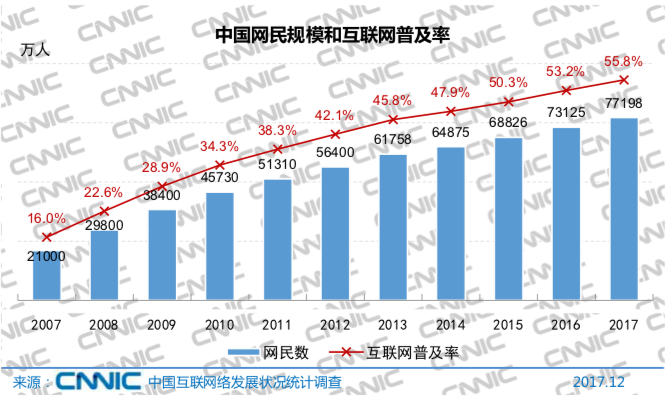
\includegraphics[width=0.8\textwidth]{1-1-1}
    \bicaption{中国网民规模和互联网普及率\citep{CNNIC}}{Chinese Internet users scale and Internet penetration rate\citep{CNNIC}}
    \label{fig:1-1-1}
\end{figure}

在不同形式的社交媒体中,微博以其独特的社交方式、巨大的网民基础和多 媒体技术之间的融合,成为当今信息产生和传播的重要平台。随着网民规模的不 断扩大,使用社交网络的用户也呈现出爆发增长的态势,微博用户逐年增加,覆 盖的群体越来越广,微博月活跃用户如图\ref{fig:a}所示。微博平台的用户不仅是信息 的接受者,同时可以是信息的产生者和传播者。这种“去中心化”的信息传播模式 使得信息可以在短时间内迅速在社交网络上广泛传播,从而产生巨大的社会影 响。

\begin{figure}[H]
    \centering
    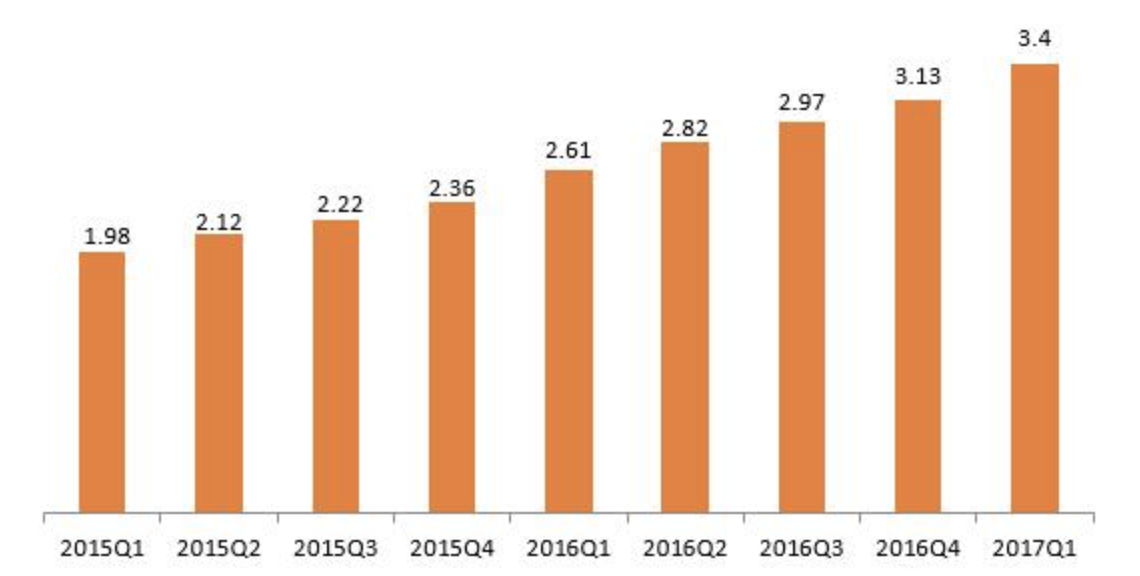
\includegraphics[width=0.6\textwidth]{a}
    \bicaption{微博月活跃用户\citep{weibo}}{Microblogging monthly active users\citep{weibo}}
    \label{fig:a}
\end{figure}


微博等社交应用的出现极大地降低了社会网络中用户间信息交流的成本,大 量用户通过社交网络积极地参与信息传播,使得社交平台上的信息传播呈现出 传播速度快、覆盖范围广和社会影响力深等特点;在传播范围上,社交信息的传 播还具有流行度呈现幂律分布的特点 \citep{Bakshy2011Everyone},即仅有少部分信息能够被大量用户转 发,而大部分信息只有很少的人会关注,不会变得流行。产生这种现象的主要原 因是社会网络中的信息存在过载问题,使得用户注意力成为稀缺资源 \citep{Davenport2001The},信息 只有在引起足够多用户关注的前提下才能够生存并继续传播。

微博作为社会交流和信息传播的主要平台之一,已经成为国内网络用户的 主要信息来源。在微博的消息传播中常出现消息的阵发性现象,即一个讨论的话 题的产生到流行,会在一个短时间内发生,然后很快就会消失。这样的突发话题 通常是由突发新闻、真实事件、恶意谣言或各种各样的行为引发的。这些爆炸性 的话题,通常被称为热门话题,为用户提供最新的事件。因此预测热门话题在很 多方面至关重要,如销售、股票市场、搜索引擎查询、选举,甚至是疾病爆发。 因此,更早的发现这些突发事件意味着增加收入,减少损失,及时治疗,以及更 好的决策。但同时由于这种话题的阵发性,导致了阵发话题的预测存在相当的困 难。

在微博和 Twitter 中,主题标签通常以 Hashtag 作为标识\citep{shaojian2}。在微博或是 Twitter 用户发送的消息中,带有以 \# 开头和结尾的文字即便认为该消息带有主 题标签,各种主流微博平台都提供了 Hashtag 标注功能,如关于马航坠机事件的 Hashtag 在 Twitter 中为“\#MH370”,在新浪微博中为“\#MH370\#”。虽然不同平台 中 Hashtag 的具体标记形式可能不同,但功能基本相同,都具有主题标注和话题 参与的功能。主题标注功能指 Hashtag 能够表达一条微博中的主题信息,话题参 与功能指用户使用 Hashtag 参与同一个话题的讨论。在微博平台中,上述功能使Hashtag 在信息组织和信息检索方面具有优势,因此越来越多的学者开始深入研究 Hashtag。


\section{研究意义}

根据从微博的数据中分析得到,我们每天可以识别数十万个新 Hashtag。 Hashtag 作为一个用户自发打下的标签,表达了用户真实想法,对于捕捉用户 兴趣和关注有极大作用。并且在微博上 Hashtag 的流行度反映了当下的社会群体 的关注点,表述了网民对于事件的重视程度。如图\ref{fig:b}所述,十九大期间,“\# 十九 大 \#”这个 Hashtag 出现了几十亿次,直观的反映了人们对于该事件的关注程度。 因此 Hashtag 在突发事件监测 \citep{Hughes2009Twitter}、流行电视节目评论监测 \citep{Deller2011Twittering} 和公众对政府的态 度监测 \citep{small2011hashtag}等方面发挥重要的作用。本文从微博的实际场景出发,根据 Hashtag 的自身特性进行相关研究,构建 Hashtag 的流行度预测,关注其未来趋势,对于 发现热门话题十分重要。

\begin{figure}[!htbp]
    \centering
    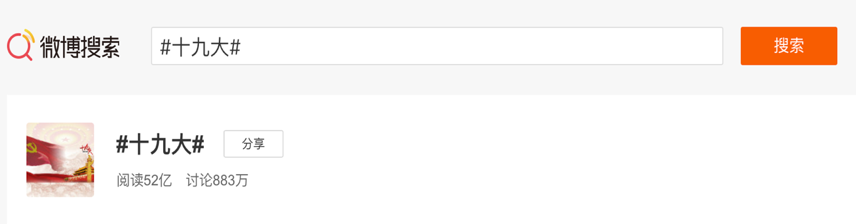
\includegraphics[width=0.8\textwidth]{b}
    \bicaption{Hashtag 热度展示}{Hashtag heat display}
    \label{fig:b}
\end{figure}

\section{面临的问题和挑战}
结合上述背景,本文的任务为 Hashtag 流行度预测,并将其应用在事件流行 度预测模型中,所面临的主要问题和挑战有以下两点:
\begin{enumerate}
\item 现有的社交网络的 Hashtag 流行度预测问题没有考虑用户之间的社交网 络结构特征以及 Hashtag 自身的特性。当前的流行度预测问题,主要考虑的 Hash- tag 的时间序列特征以及 Hashtag 的内容特征,例如考虑时间间隔内 Hashtag 的 转发次数,来预测接下来的转发情况,当然时间序列特征是一个直观并且比较有 效的特征,它很好的反映了消息一个时间段的热门程度。但是 Hashtag 本身是由 用户产生并且进行转发的,用户之间的关注关系是十分重要。并且 Hashtag 有其 自身特性,比如情感性,地域性以及事件性,这些都是其自身重要的特征,对于 预测 Hashtag 的流行度具有很大作用。因此,本文希望在现有的特征的基础上考虑用户的网络结构特征以及 Hashtag 的自身特性,更好的进行 Hashtag 流行度预 测。
\item 传统的消息流行度预测都是单源问题,即消息都是由一个个体发出然后 进行转发传播,但是相同的 Hashtag 可以由不同的个体从不同的时刻发出,如何 处理多源 Hashtag 是本文面临的一大挑战。本文希望通过给出合适的 Hashtag 流 行度预测模型,更好地处理多源消息的预测问题。
\end{enumerate}

\section{论文的研究内容}
本文以面向主题标签流行度预测为研究主体,并实现与之对应的事件流行
度预测框架。针对 1.3 中涉及的问题,本文的研究内容将主要包括以下三个方面:
\begin{enumerate}
\item 在传统的基于特征的 Hashtag 流行度预测的基础上结合用户社交网络结 构信息以及 Hashtag 自身特性,进行更加全面的流行度预测算法。
\item 从消息单源特性出发,考虑 Hashtag 的多源性,结合 Hashtag 传播过程中 的时间因素,实现基于多源头的 Hashtag 流行度预测算法。

\item 整合基于特征的 Hashtag 流行度预测算法,考虑性能以及用户群体等信 息,实现完整的具有较高预测性能的事件热度预测框架。
\end{enumerate}


\section{论文的贡献}
基于 1.4 中的研究内容,本文的贡献主要有以下几点:
\begin{enumerate}
\item 从Hashtag自身特性以及用户粉丝的网络结构特性出发,对已有的微博文 本以及时间序列特征进行扩充,利用用户粉丝的网络结构向量特征,以及 Hashtag 的情感性,地域性,人物性等特征进行模型训练。实验结果表明,新提出来的特 征对于 Hashtag 的流行度预测问题有了一定的效果,也即证明新提出的特征有效 的表达了 Hashtag 的传播特性。
\item 结合外部知识,利用已知的用户粉丝网络结构,提出多源的 Hashtag 流 行度预测模型:利用已知的用户粉丝网络结构,学习用户的向量表达,将其和 Hashtag 的传播路径作为模型的输入进行训练学习,实现用户粉丝网络结构和多 源模型的整合。在大规模微博语料上,对多源 Hashtag 流行度预测模型进行了实 验验证。实验结果表明,模型可以有效地处理多源头的 Hashtag 流行度预测问题。

\item 事件热度预测系统的实现与部署,论文考虑到 Hashtag 可以作为微博中 的事件或者话题,采用基于特征的 Hashtag 流行度预测模型,搭建了事件热度预 测系统。事件热度预测系统通过自动分析微博数据,利用本文提出的主题标签流行度预测算法,进行事件热度预测,通过系统验证了模型的有效性。结果表明,本文提出的事件热度预测具有较高的应用价值。

\end{enumerate}

\section{论文的组织结构}
论文共分为六个章节,主要内容有:

第一章介绍本文的研究背景、研究内容和主要贡献,并给出了本文的组织结 构。

第二章介绍了与本文研究内容相关的流行度预测的相关工作和国内外研究 现状。基于特征的流行度预测方面介绍了现有的流行度预测所考虑到的特征以 及使用的模型;基于消息传播过程的方面分别介绍了点过程以及深度学习方面 的应用。

第三章提出了基于用户网络结构特征以及主题标签自身特性的主题标签流 行度预测算法。从宏观角度出发,不考虑 Hashtag 的传播过程,利用机器学习, 考虑用户粉丝网络结构特征以及 Hashtag 情感性,地域性等特征,采用 xgboost 模型进行 Hashtag 流行度预测;最后通过实验验证模型的有效性。

第四章提出了多源头的主题标签流行度预测。从微观角度出发,考虑 Hashtag 的传播过程,针对 Hashtag 的多源性使用循环神经网络模型,刻画 Hashtag 的传 播过程,结合用户的网络结构特征作为先验知识,进行 Hashtag 流行度预测;最 后通过实验验证模型的有效性。

第五章提出了主题标签流行度预测在事件热度预测系统中的应用。考虑 Hashtag 可以作为微博消息的事件或者话题的特性,采用基于特征的 Hashtag 流 行度预测方法,利用多种组合特征,采用机器学习模型,实现了事件热度预测系 统;最后通过实际应用验证了该模型的有效性和实用性。

  第六章总结了本文中的工作,并对未来研究工作进行了展望。
\chapter{相关工作及国内外研究现状}\label{chap:two}
微博平台已经在越来越多的使用 Hashtag,Hashtag 的研究涉及方方面面,对 其研究有重要意义与价值。Hashtag 的流行度是 Hashtag 的基本特性,对其进行 深入研究,可以预测哪些话题会成为热门,对于突发事件的预测有重要帮助。

本文主要研究 Hashtag 的流行度预测,本章首先介绍传统的流行度预测方 法,然后介绍 Hashtag 的流行度预测的相关研究。

\section{流行度预测的方法}
微博消息的流行度预测是指微博消息在未来一段时间内的转发次数,而主 题标签的流行度预测是指该主题标签在未来一段时间内的使用情况,既包括转 发也包括原发。现有的流行度预测方法主要分为两类: 基于特征的方法和基于生 成方法。基于特征的方法主要是根据长时间的观测数据,提取消息的静态和动态 传播特征,如消息的内容特征,时序特征,用户特征,传播相关的社交网络结构 特征等,然后采用机器学习模型进行预测,而基于生成方法是刻画消息内部的传 播机制,深刻理解消息的传播过程。近年来,基于神经网络的表示学习的方法具 有显著的预测能力,这方面的研究日趋增多。

\subsection{基于特征的方法}
基于特征的方法通常认为流行度预测任务是一个回归问题 \citep{szabo2010predicting,pinto2013using}或者分类 问题 \citep{Cheng2014Can,Shulman2016Predictability}。这些方法为流行度预测提取了各种人工构造的特征,这些特征通常 被绑定到特定的数据集或社交媒体平台上,比如 Twitter\citep{Bakshy2011Everyone},Digg\citep{szabo2010predicting} 和 Youtube \citep{szabo2010predicting,pinto2013using}。这些特征主要包括时间特征\citep{szabo2010predicting,pinto2013using},结构特征 \citep{romero2013interplay},内容特征\citep{tsur2012s}以 及早期传播者的特征。Szabo 等 \citep{szabo2010predicting}观察到,在线内容的未来流行度与它早期的 流行程度成线性相关。后来,Pinto 等 \citep{pinto2013using}通过在观察时间内,以相同大小的时 间间隔代替了早期累积受欢迎度,从而扩展了该模型。综上所述,基于特征的方 法为我们提供了对流行度预测的一般理解,展示了结构、时间、内容和早期传播 者的特征。然而,它们的性能很大程度上取决于提取的特征,这很难设计和测 量。因此对于可以自动学习有效特征的模型是目前研究的方向。


\subsubsection{基于分类模型的方法}

基于分类模型的方法将微博流行度预测问题转换为分类问题,利用大量的 已知数据抽取特征,然后利用这些特征训练出机器学习模型,将微博流行度分为 多个级别并打上标签,但是目前没有统一的分类准则。Hong 等 \citep{hong2011predicting}把信息是否 能转发看作是二分类问题,进一步用多分类方法预测信息的流行程度,使用逻辑 回归模型对两个任务进行了建模:一个是预测目标消息是否会被转发,为一个二 分类问题;另一个是预测目标消息的最终转发范围,为一个多分类问题。该方法 分析了社交网络中的各种特征对消息传播的影响,具有一定的启示意义。Wang 等\citep{hong2011predicting} 主要是挖掘了微博内容的文本特征和语法特征,并利用机器学习中的决 策树模型和支持向量机模型预测微博转发数。Lakkaraju 等人 \citep{Lakkaraju2011Attention}利用支持向量 机模型把微博关注度分为非常少、少、一般、高和非常高 5 类,根据定义好的分 类准则然后进行分类模型的训练。

\subsubsection{基于回归模型的方法}

基于回归模型的方法试图找到影响因素与微博信息流行度之间的相关关系, 进而使用线性回归或非线性回归模型进行微博信息流行度的预测。Szabo 等人 \citep{szabo2010predicting} 研究了社交网络 Digg 和 YouTube 上的流行度预测问题,实验表明,消息早 期流行度的对数和未来流行度的对数之间存在很强的相关性,如图\ref{fig:digger-youtube}所示。
\begin{figure}[H]
    \centering
    \begin{subfigure}[b]{0.5\textwidth}
      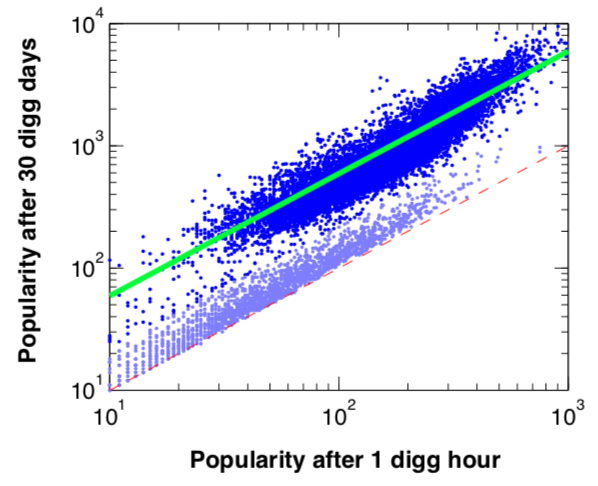
\includegraphics[width=\textwidth]{digger}
      \caption{}
      \label{}
    \end{subfigure}%
    ~%add desired spacing
    \begin{subfigure}[b]{0.5\textwidth}
      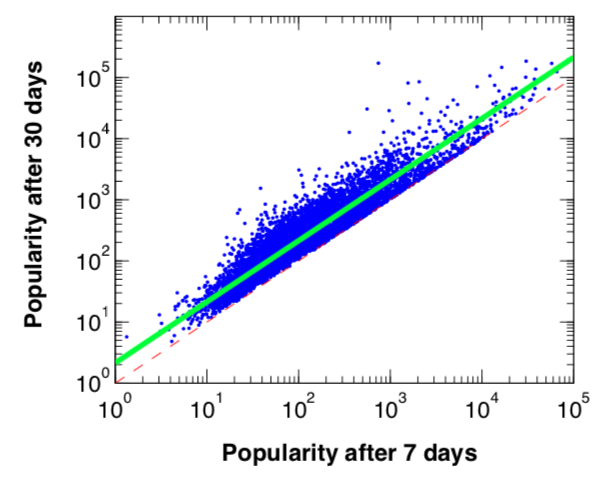
\includegraphics[width=\textwidth]{youtube}
      \caption{}
      \label{}
    \end{subfigure}
    \bicaption{消息流行度展示。(a)Digg 数据集,(b)Youtube 数据集。\citep{szabo2010predicting}}{Message popularity display. (a)Digg data, (b) Youtube data.\citep{szabo2010predicting}}
    \label{fig:digger-youtube} 
\end{figure}

Lee 等 \citep{Lee2010An}认为在线文本的流行度有时本身就不能被预测,所以没有预测 在线文本的流行度而是利用比例风险回归模型对文本早期信息的特征进行研究,预测其是否会流行。Jamali 等 \citep{Jamali2009Digging}使用 Digg 信息的评论数量、评论的平均字数 和评论树状结构作为特征,训练他们的回归模型。Tatar 等 \citep{Tatar2011Predicting}用信息在其发布 的一段时间后获得的评论数作为因子,提出了一个简单有效的线性回归模型,预 测其后期的流行度。Bao 等人 \citep{Bao2013Popularity,Gao2014Popularity}研究了以微博消息为研究对象,研究了消 息流行度预测与消息早期传播的网络结构之间的关联性,如图\ref{fig:str}所示,消息未 来的流行度与消息早期传播的链接密度存在很强的负相关性,和消息早期的传 播深度存在近似的线性相关性。于是,基于初始阶段用户之间链接密度和微博的 传播深度,分别提出了两个微博流行度的预测模型。第一个模型是在微博转发 的初始阶段,基于微博的转发深度来预测微博的转发量;第二个模型是在微博 转发的初始阶段,基于用户的链接密度来预测微博的转发量。Cheng 等 \citep{Cheng2008An}采用 了时间序列模型中常用的自回归移动平均模型 (Autoregressive Integrated Moving Average Model,ARIMA),对网络上跟帖数量随时间变化的趋势情况进行了预测 分析。

 
 \begin{figure}[H]
    \centering
    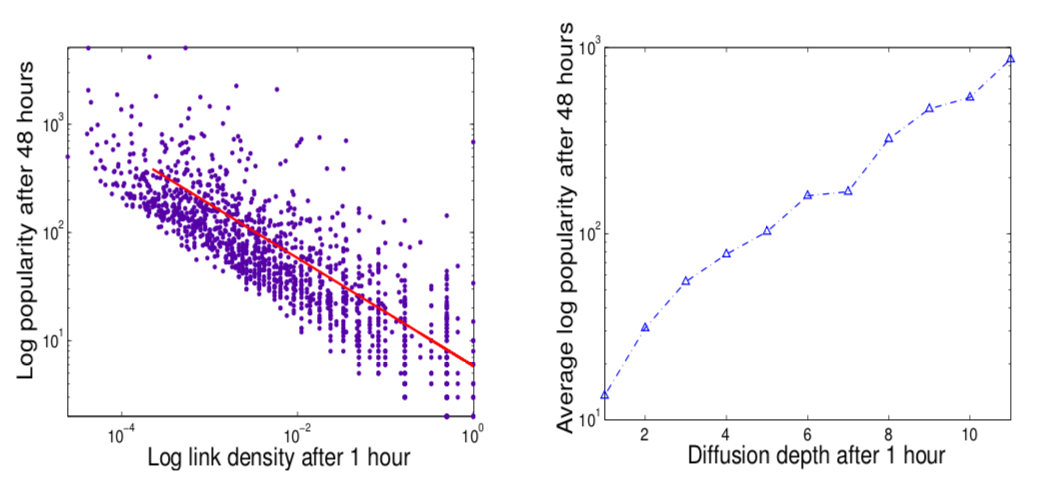
\includegraphics[width=0.5\textwidth]{str}
    \bicaption{结构特性\citep{Bao2013Popularity}}{Structural characteristics\citep{Bao2013Popularity}}
    \label{fig:str}
\end{figure}

\subsection{基于时间序列的方法}
基于时间序列建模的预测方法主要关注用户传播过程对应的时间序列。这 类方法在对时间序列建模后,利用所得的模型进行用户生成内容的流行度预测 工作。Yang 等 \citep{Yang2011Patterns} 研究了用户生成内容流行度随时间的消涨模式。该研究利 用 K-谱中心聚类算法和逻辑回归模型,通过对 5.8 亿条推文和 1.7 亿篇博客文 章流行度随时间消涨模式的聚类分析,挖掘出 6 类形态各异的流行度时序模式。 Matsubara 等 \citep{Matsubara2012Rise}做了进一步研究,用 SpikeM 模型对上述 6 种时序模式进行拟 合,利用 SpikeM 模型进行流行度预测。SpikeM 模型利用幂律分布描述用户生成 内容的传播能力随时间衰减的过程,并利用正弦方程描述用户关注度随时间周 期变化的过程。Figueiredo 等 \citep{Figueiredo2014TrendLearner}利用极随机集成树将时间序列分类,从而预测 信息的趋势。Hu 等 \citep{Hu2016Predicting}通过对短期爆发的热门话题流行度时间序列进行分析,发现这些序列具有高度相似性,进而定义流行度时序特征空间,即流行度的平均 值、走势和周期,以分析流行度随时间的变化趋势。

\subsection{基于传播模型的方法}

传播模型最早是流行病学中对病毒扩散机制的研究,社交网络中的消息传播机制可以和病毒在人群中的传播方式进行类比。两者的不同之处在于,社交 网络是存在一定的网络结构的,消息一般是沿着社交网络结构进行扩散。并且, 用户之间的消息传播概率和病毒传播的概率也有较大区别。传播过程分析和动 力学研究是预测信息流行度的重要基础。以生物数学领域中的流行病模型为基 础,构建新的传播规则和模型是微博流行度预测的一种重要方法。这些模型通 常把微博网络中的用户节点划分为未知者、传播者和免疫者三大类。在消息传 播网络中,给定一条微博消息,未知者表示从没有接触过该消息的用户,传播者 表示接触过该消息并且以一定概率传播该消息的用户,免疫者表示了解消息但 不会进行传播的用户。在消息传播过程中,传播行为主要发生在不同状态节点 相互连接所产生的边。在 Daley 等人 \citep{Daley1965Stochastic}提出的 DK 模型中,若传播者遇到未 知者,未知者则以一定的概率变为传播者;若传播行为发生在 2 个传播者之间 时,两者都会以一定概率转化为免疫者。Maki 等人 \citep{Maki1973Mathematical} 提出的 MK 模型的传播 规则有所不同,即当 2 个传播者相遇时,只有一个传播者以一定概率变为免疫 者。Xiong 等人 \citep{Xiong2012An}将用户分为易感染人群、接触信息人群、感染人群和康复人 群类,建立了基于转发机制的信息传播模型。研究结果发现,无标度网络中的接 触信息人群比规则网格中的多;感染者的密度随着点度的增加而增长。Wang 等 人\citep{WANG2013ReTweeting} 发现微博传播与 SIS(susceptible-infectious-susceptible) 模型存在许多相似 性,因而利用 SIS 模型预测微博转发行为,实验结果显示,预测的错误率很低。 Yang 等人\citep{Yang2011Modeling} 在 SIS 模型的基础上提出了线性影响模型,根据当前微博信息的 流行度预测未来某一时间的流行度。模型假设微博信息的传播受各节点影响力 支配,为每个节点建立影响函数以量化该节点对后续被激活节点的影响力,从而 把流行度预测转换为活跃节点的影响力计算问题。


基于传播模型的方法还有一种是将在线内容的受欢迎度累积为转发过程,并 对每个消息的到达过程中的强度函数进行独立的建模。Shen 等 ­\citep{Shen2014Modeling} 采用了强化 泊松过程 (Reinforced Poissopn Process,RPP) 来对社交网络中的三种现象进行建 模: 一个消息的固有吸引力,对吸引力的短暂放松,以及富者愈富的机制,公 式如\ref{eq:xd}所示,$i_d(t)$就是富者愈富的影响,其概率图表示如图\ref{fig:c}所示。


\begin{equation}\label{eq:xd}
\lambda_d(t) = \lambda_d f_d(t,\theta_d)i_d(t)
\end{equation}



其中,$\lambda_d$为消息的固有吸引力,时间松弛函数 (temporal relaxation function)  $f_d(t,\theta_d)$刻画了吸引力时效性对消息传播速率的影响,$\theta_d$为松弛函数的参数,$i_d(t)$
表示消息 \textit{d} 在时刻 \textit(t) 已经收到的关注数。该模型在论文引用网络中进行了验证, 其中,时间松弛函数如公式\ref{eq:fd}, 反映了论文影响力的时间衰减效应。此处,自增 强采用的是线性函数,反映了论文吸引力随着引用次数的增加呈线性增长。

\begin{equation}\label{eq:fd}
f_d(t) = \frac{1}{\sqrt{2\pi}  \sigma_dt}\exp(-\frac{(\ln t - \mu_d )^2}{2\sigma_d^2})
\end{equation}

\begin{figure}[H]
    \centering
    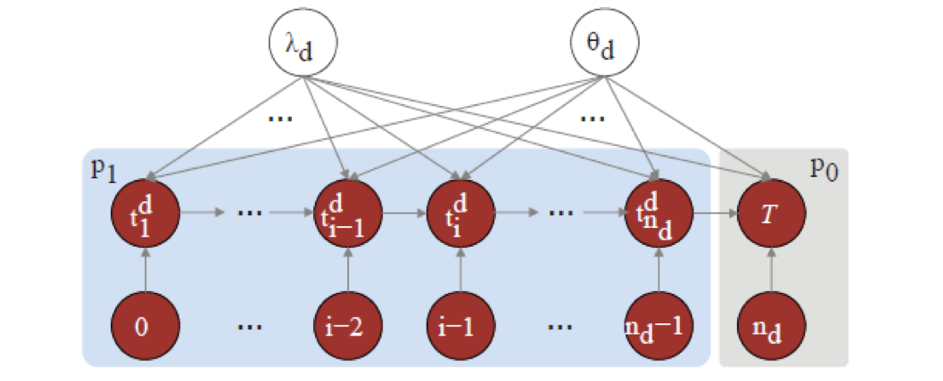
\includegraphics[width=0.5\textwidth]{c}
    \bicaption{RPP概率图\citep{Shen2014Modeling}}{RPP probability graphical\citep{Shen2014Modeling}}
    \label{fig:c}
\end{figure}


Gao 等人\citep{Gao2016Modeling}在研究中发现消息传播中关键用户的影响,提出了混合的 RPP 模型,将消息的传播看成是多个由关键用户节点引起的 RPP 子过程的混合,如 图\ref{fig:d}所示。将 RPP 模型扩展到不同的时间松弛函数,并将其应用于动态转发过 程的预测。后来,利用 RPP 模型中的转发数量,来模拟富者愈富的现象,利用 Hawkes 自激励点过程直接对每个消息转发的具体贡献进行建模,其特征为用户 影响和时间松弛函数。Hawkes 过程为我们提供了一个通用的框架来建模一个信 息如何引起注意的过程,这使我们非常容易理解信息级联的底层机制。此外,还 采用深度学习技术来学习到达率在点过程中的作用。无论如何,这些方法通常 不会对未来的流行度进行直接优化,并且这些方法是独立地为每个消息学习参 数,缺乏实际应用能力。因此,他们不能充分利用流行度预测中的隐含的级联 信息, 在可解释性和可预测性之间仍然存在差距。为了解决这一难题,通过学习 Hawkes 过程的内部因素,即: 在端到端监督框架下,用户影响、自激励和时间衰 减等不同的因素的影响,为流行度预测的可解释性和可预测性提供更好地解决 方案。

\begin{figure}[!htbp]
    \centering
    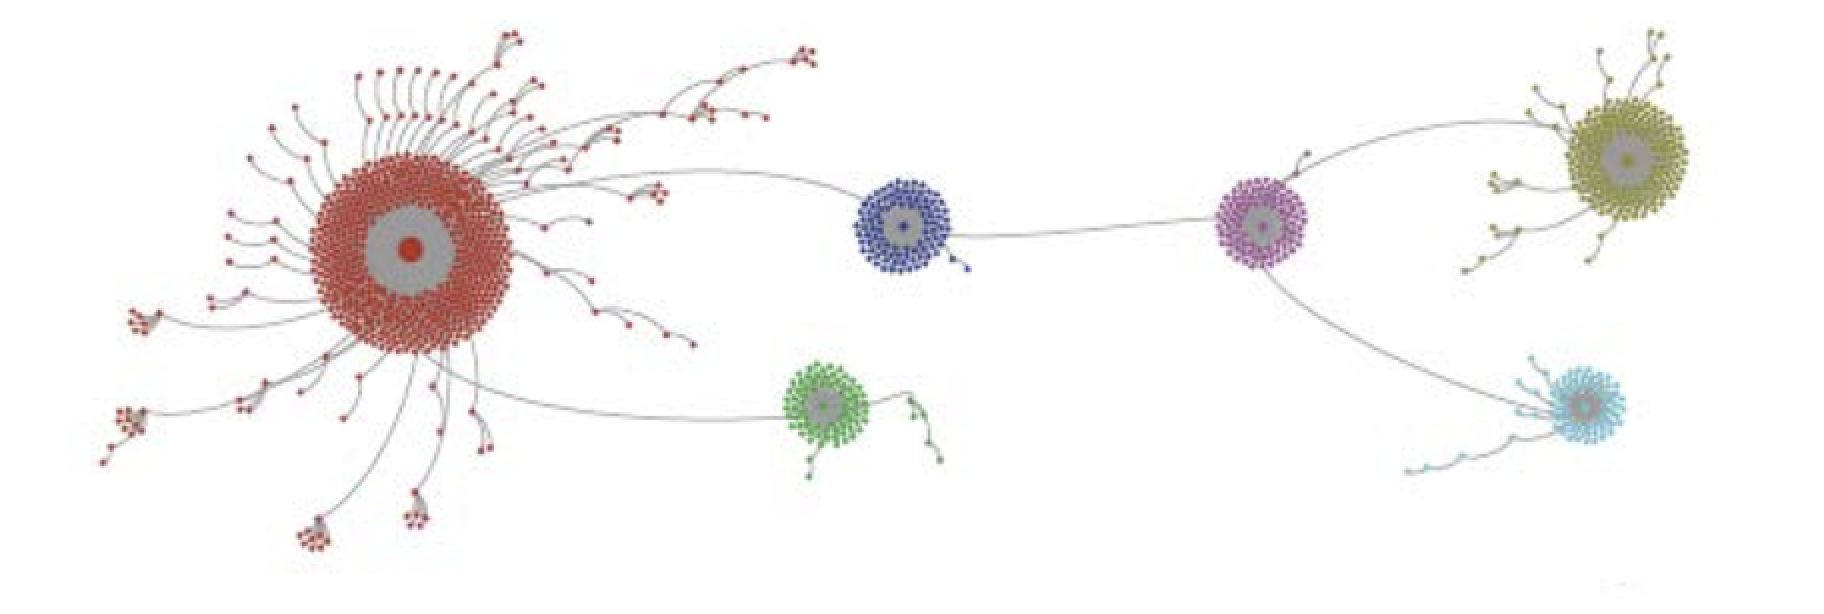
\includegraphics[width=0.7\textwidth]{d}
    \bicaption{新浪微博中某消息的传播拓扑结构图\citep{Gao2016Modeling}}{A Topology Of The Spread Of A Message On Sina Weibo\citep{Gao2016Modeling}}
    \label{fig:d}
\end{figure}

\section{深度学习背景}
近年来,深度学习作为一个强大的工具在多个领域取得了成功的应用,在社 交网络领域,也有不少相关的尝试,均取得了不错的效果,说明了深度学习模型 在社交网络分析领域有巨大的运用价值。在消息传播预测中,消息的传播过程就 是一个明显的序列过程,将消息在用户之间的互相传播过程解析成一系列的序 列过程,在这个过程中,应用深度学习中的循环神经网络处理是十分方便的,因 此深度学习在消息预测中有着十分广阔的应用。
\subsection{深度学习简介}
深度学习是利用一个层次化的架构学习出原始输入在不同层次上的表达,在 这个层次化中,高层的概念通常是通过低层的概念来定义的,这种层次化的表达 可以帮助解决更加复杂抽象的任务。深度学习通常使用人工神经网络,常见的具 有多个隐层的深度神经网络 (DNN) 就是典型的深度架构。很多深度学习模型有 其仿生学基础,因为人的信息处理系统是清晰的层次化的结构,比如人类的听觉 系统以及视觉系统,所以很自然地,人们相信如果能够构造类似的深度架构和相 应的学习算法会对处理这种类型的自然信号有很大的帮助。此外,从理论角度, 这种层次化的结构在表达某些特定运算的时候往往能够比浅层架构更加高效。

深度学习一直面临着计算量大、难以优化以及容易过拟合等问题。转机出现 在 2006 年,一直致力于神经网络以及深度学习研究的 Hinton 等人使用无监督的 逐层处理的预训练方法成功减轻了深度模型学习困难的问题,从而掀起了深度 学习的浪潮 \citep{Sch2006Efficient}。近年来,随着计算能力的不断提升、数据量的不断增加以及新 的训练方法的提出 \citep{Srivastava2014Dropout},深度学习得到进一步发展,深度模型的效果也越来越明 显,最终在语音识别、自然语言处理和图像处理等一系列难题上取得了巨大的突 破,并得到了学术界和工业界的广泛重视。在语音领域,从 2009 年开始,微软 研究院和 Hinton 合作率先在语音处理中使用深度神经网络,从而使得语音识别成为深度学习取得突破的第一个领域 \citep{Hinton2012Deep,Deng2013New}。在图像领域,2012 年,Hinton 团 队的 Krizhevsky 等人 \citep{Krizhevsky2012ImageNet}  使用深层次的卷积神经网络在 ImageNet 评测上取得巨 大突破,将错误率从 26\% 降低到 15\%,重要的是,这个模型中并没有任何手工 构造特征的过程,网络的输入就是图像的原始像素值。在此之后,采用类似的架 构,通过使用更深更复杂的模型、更多的参数以及训练数据,ImageNet 评测的 结果得到进一步大幅改善。这期间典型的模型包括 Google 构建的 24 层的深度神 经网络 GoogLeNet\citep{Szegedy2015Going}以及微软构建的 152 层的深度网络  \citep{He2016Deep,He2016Identity} 等。

\subsection{循环神经网络概述}

循环神经网络(recurrent neural network,RNN)是上世纪 80 年代末提出的 一种针对处理时间序列输入的神经网络。循环神经网络相对于传统的前馈神经 网络主要具有以下特点:(1) 前馈神经网络的网络拓扑结构构成了一个有向无环 图,信息沿着一个方向从输入节点传递到输出节点。循环神经是一种带环的神 经网络,网络中产生的信息会反馈到后面的计算中。(2) 前馈神经网络主要处理 静态的输入输出数据,而循环神经网络主要用来模拟动态系统或者建模变长序 列数据。RNN 的这种环状连接在网络内部构成一种用来刻画动态变化的状态信 息。RNN 可以用这种内部状态存储机制来处理任意的序列输入。因此 RNN 适用 于很多序列相关的应用,比如语音识别、自然语言理解等。(3) 循环神经网络可 以按照序列顺序,展开得到一个前馈神经网络的形式,但是由于 RNN 每一步计 算中采用同样的函数,因此,循环神经网络可以认为是一种在所有层之间共享参 数的前馈神经网络。基础的 RNN 的计算公式如\ref{eq:2-rnn}所示, 其中,$h_t$为 t 时刻的表 达,$x_t$ 为 t 时刻的输入,W,U,b 是模型的参数。

\begin{equation}\label{eq:2-rnn}
h_t = g(Wx_t + Uh_{t-1} + b)
\end{equation}

前馈神经网络主要基于反向传播进行梯度求解 \citep{Rumelhart1988Learning,Werbos1994The}。由于循环神经网络 可以认为是共享参数的前馈神经网络,因此主要采用时序反向传播算法。这种算 法是传统反向传播算法的一种扩展。我们先将一个循环神经网络展开成共享参 数的前馈神经网络,然后,基于这个前馈神经网络进行后向传播。最后,把每一 层中相应的参数梯度相加,则得到该共享参数的梯度。有时候展开得到的前馈神 经网络可能太长,因此常用的训练方法还有截断的时序后向传播算法。
\subsection{基于表示学习的方法}
由于社交网络的开放性和复杂性,网络内容的流行度预测是十分困难的。影响网络内容的未来流行程度有各种各样的因素。为了处理这种复杂的流行动态, 并从原始数据中自动提取有用的信息,基于表示学习的方法正在应用到流行度 预测中。Mishra 等人 \citep{Mishra2016Feature}提出了一种两阶段模型,将 Hawkes 点过程的参数作 为表示,并将其与其他提取的特征结合到机器学习模型中,来进行流行度预测。 Hoang 等人\citep{Hoang2017GPOP}提出将用户分组形成聚簇,然后采用张量分解进行预测。这个 方法实际上是学习在空间中每个消息的表示形式,它是由与用户组相对应的维 度来表示的。深度学习的成功,也激发了对级联预测的端到端表示学习框架。Li 等人\citep{Li2016DeepCas}提出了 DeepCas,其模型结构如图\ref{fig:deepcas}所示,它通过随机游走将级联图 作为节点序列,并在深度学习框架下学习每个级联的表示。

\begin{figure}[!htbp]
    \centering
    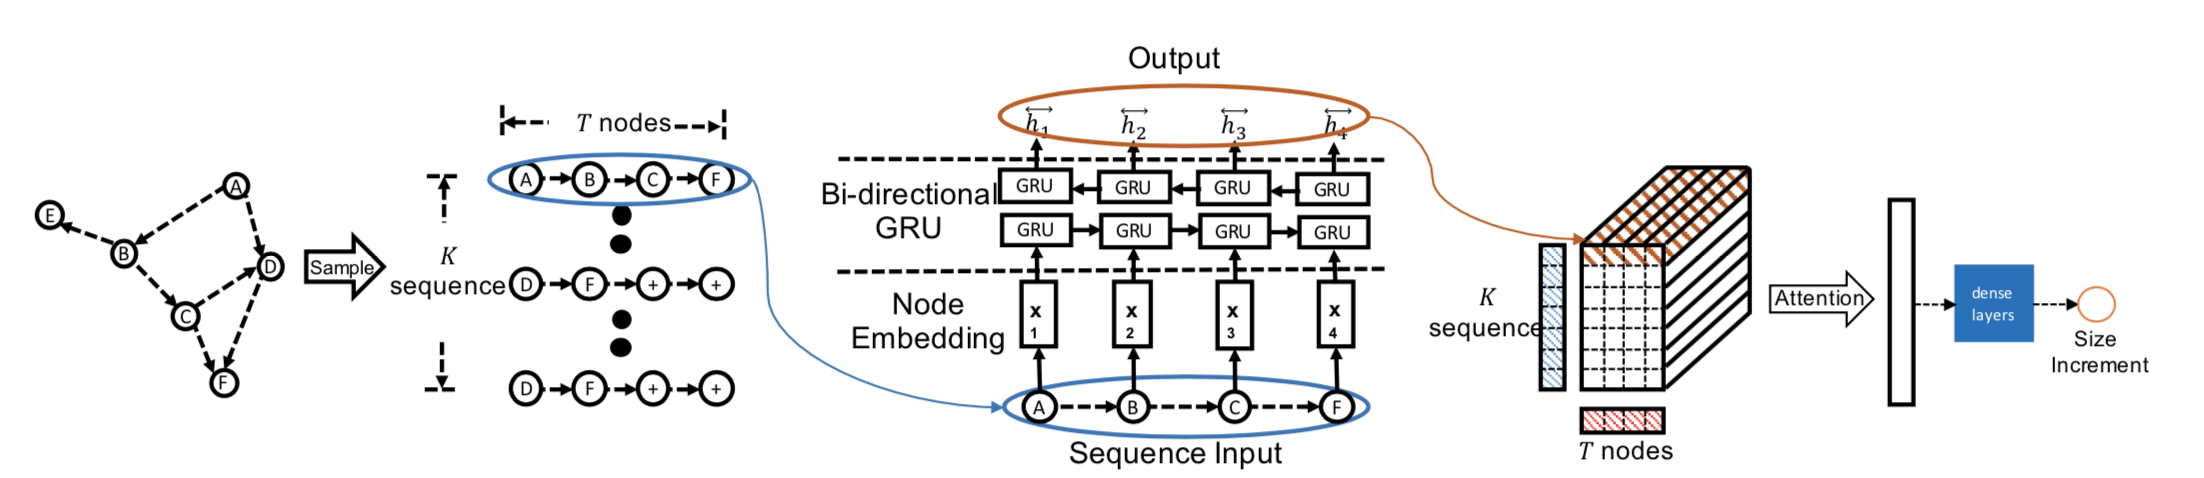
\includegraphics[width=1\textwidth]{deepcas}
    \bicaption{DeepCas模型\citep{Li2016DeepCas}}{DeepCas model\citep{Li2016DeepCas}}
    \label{fig:deepcas}
\end{figure}


表示学习的一系列的工作可以自动地从数据中学习有价值的表示,并成功 应用到其他领域的表示学习中。然而,现有的研究要么采用了两阶段的方式 \citep{Mishra2016Feature}, 缺乏作为表征学习的指南,要么忽略了传统研究所揭示的预测信息,例如,Deep- Cas\citep{Li2016DeepCas} 忽略了影响流行度预测的时间特征。此外,深度学习方法缺乏清晰的解 释性来帮助我们理解信息级联的流行动态的内在机制。在 Cao 等人\citep{Cao2017DeepHawkes}提出的 DeepHawkes 模型中,在深度学习的框架下,使用端到端的方式,直接建模未来 流行度。该方法刻画了已有的 Hawkes 模型中的信息传播过程中比较关键的因子 或机制,对未来流行度预测有很好的参考价值,其模型如图\ref{fig:f}所示。

\begin{figure}[H]
    \centering
    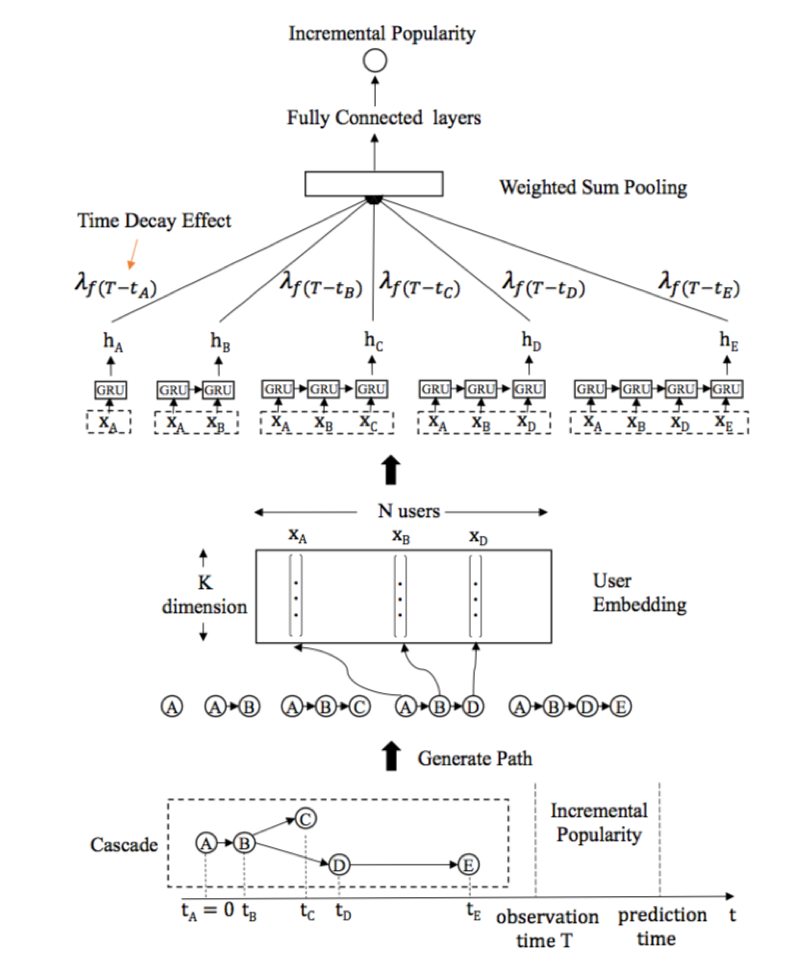
\includegraphics[width=0.5\textwidth]{f}
    \bicaption{DeepHawkes模型\citep{Cao2017DeepHawkes}}{DeepHawkes Model\citep{Cao2017DeepHawkes}}
    \label{fig:f}
\end{figure}

在社交网络消息转发预测方面,Zhang 等人 \citep{Zhang2016Retweet}主要是针对 Twitter 上消息 的转发问题进行了研究,将其建模成二分类问题,给定用户和消息,预测用户是 否会转发该消息。通过神经网络学习消息的内容表达,通过注意力机制学习用户 的兴趣表达,网络结构如图\ref{fig:dnn-attention}所示。该模型利用用户的历史发布消息学习用户 的兴趣表达,通过神经网络将转发消息有机结合起来,提高了模型的预测效果, 但是该方法与 Du 等人 \citep{Du2016Recurrent}的研究工作相比,没有考虑到消息传播中的时间序列 特征,而该特征在很多研究中已经证明了其重要性,因此该方法还有很多改进的 空间。

\begin{figure}[H]
    \centering
    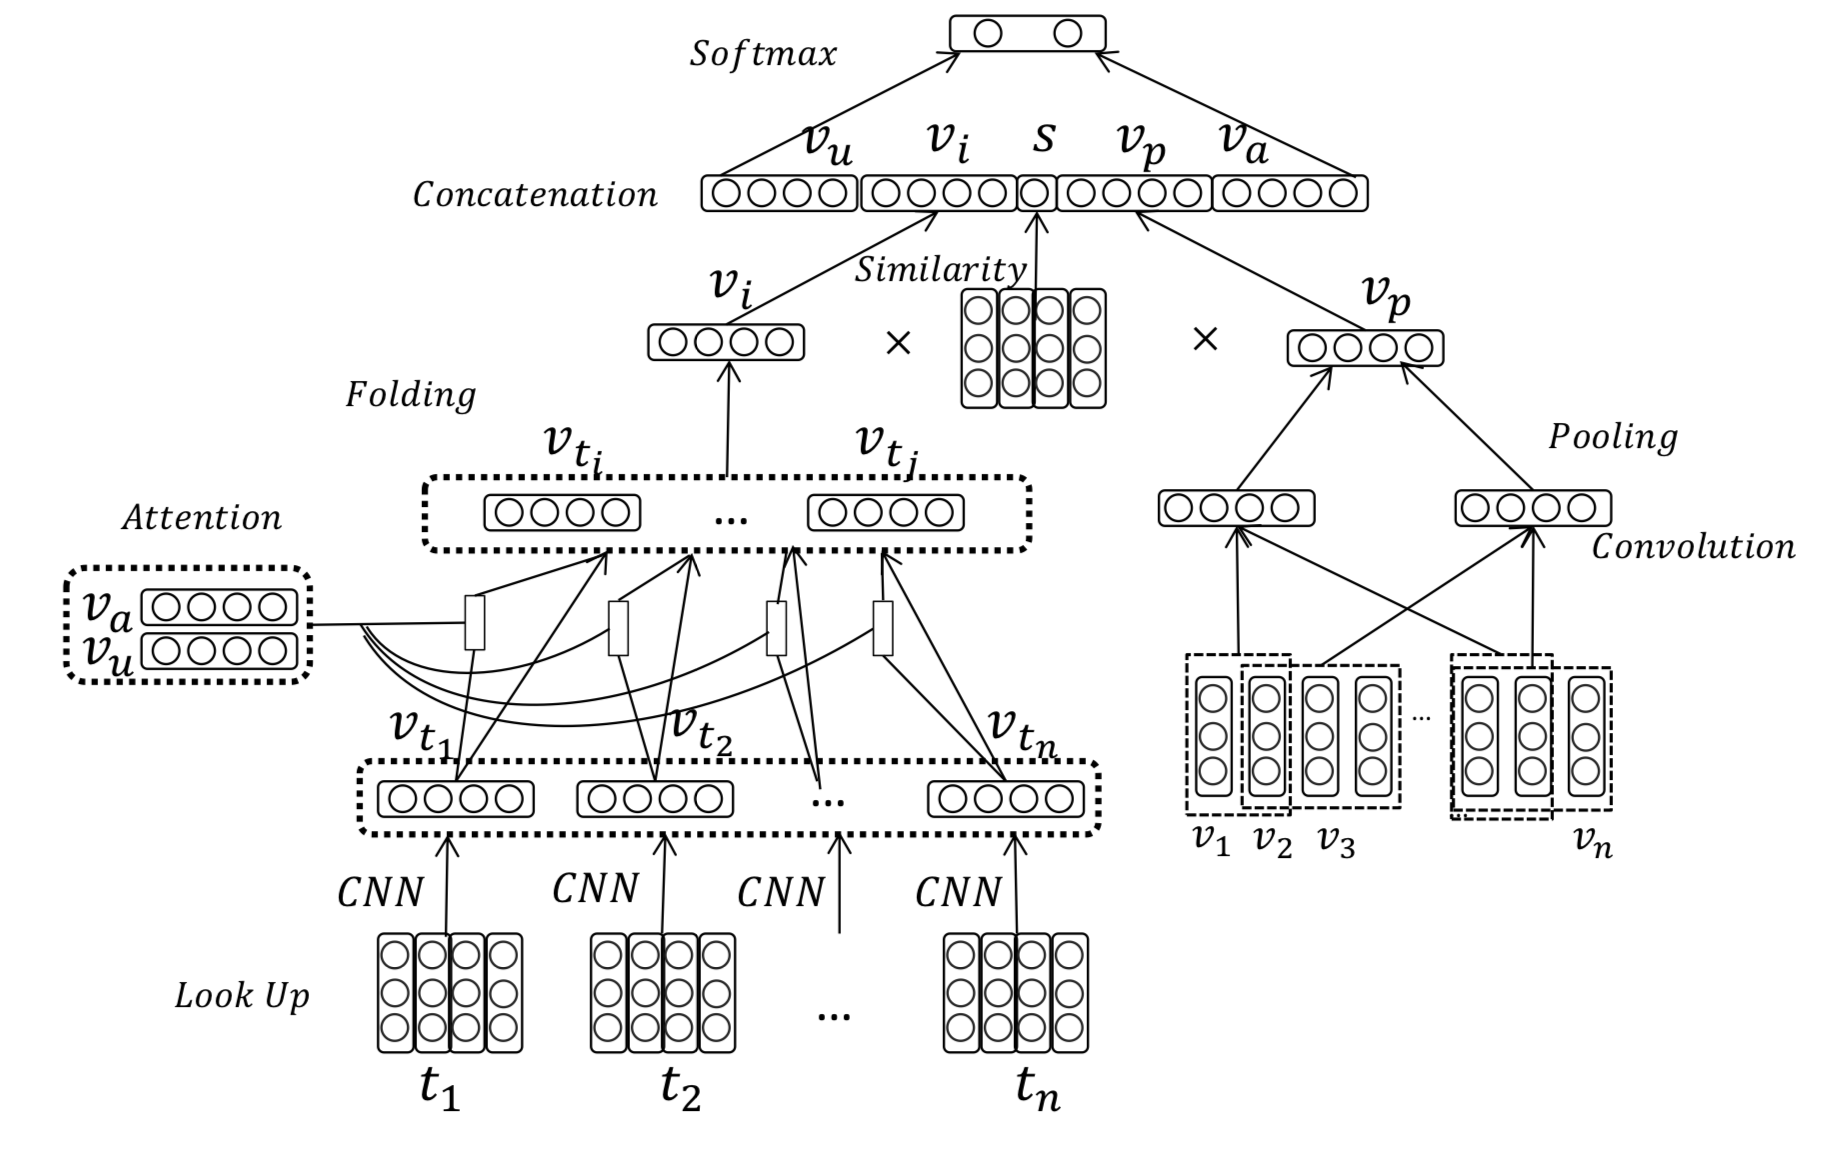
\includegraphics[width=0.8\textwidth]{dnn-retweet}
    \bicaption{基于注意力机制的预测模型\citep{Zhang2016Retweet}}{Predictive model based on attention mechanism\citep{Zhang2016Retweet}}
    \label{fig:dnn-attention}
\end{figure}

\section{Hashtag流行度预测的方法}

Hashtag 的流行度预测主要是指 Hashtag 在一段时间内被使用的情况, 这种情 况主要通过 Hashtag 的使用频次界定。Kong 等人 \citep{Kong2014Predicting}根据 Hashtag 生命周期中 的使用频次的变化情况定义了 Hashtag 的 4 种流行度类别: 出现、爆发、平静、沉 寂,Ma 等 \citep{Ma2012Will,Ma2013On} 也按照 Hashtag 的使用频率划分 Hashtag 的流行度。通过对流行 度的类别划分可以将 Hashtag 的流行度预测问题转化为分类问题, 按照不同的频 次等级对 Hashtag 进行类别划分, 使用分类器对 Hashtag 进行流行度类别的预测, 从而预测 Hashtag 在未来的使用频次,Hashtag 的分布也是呈现幂率分布的,如 图\ref{fig:g}所示。

\begin{figure}[H]
    \centering
    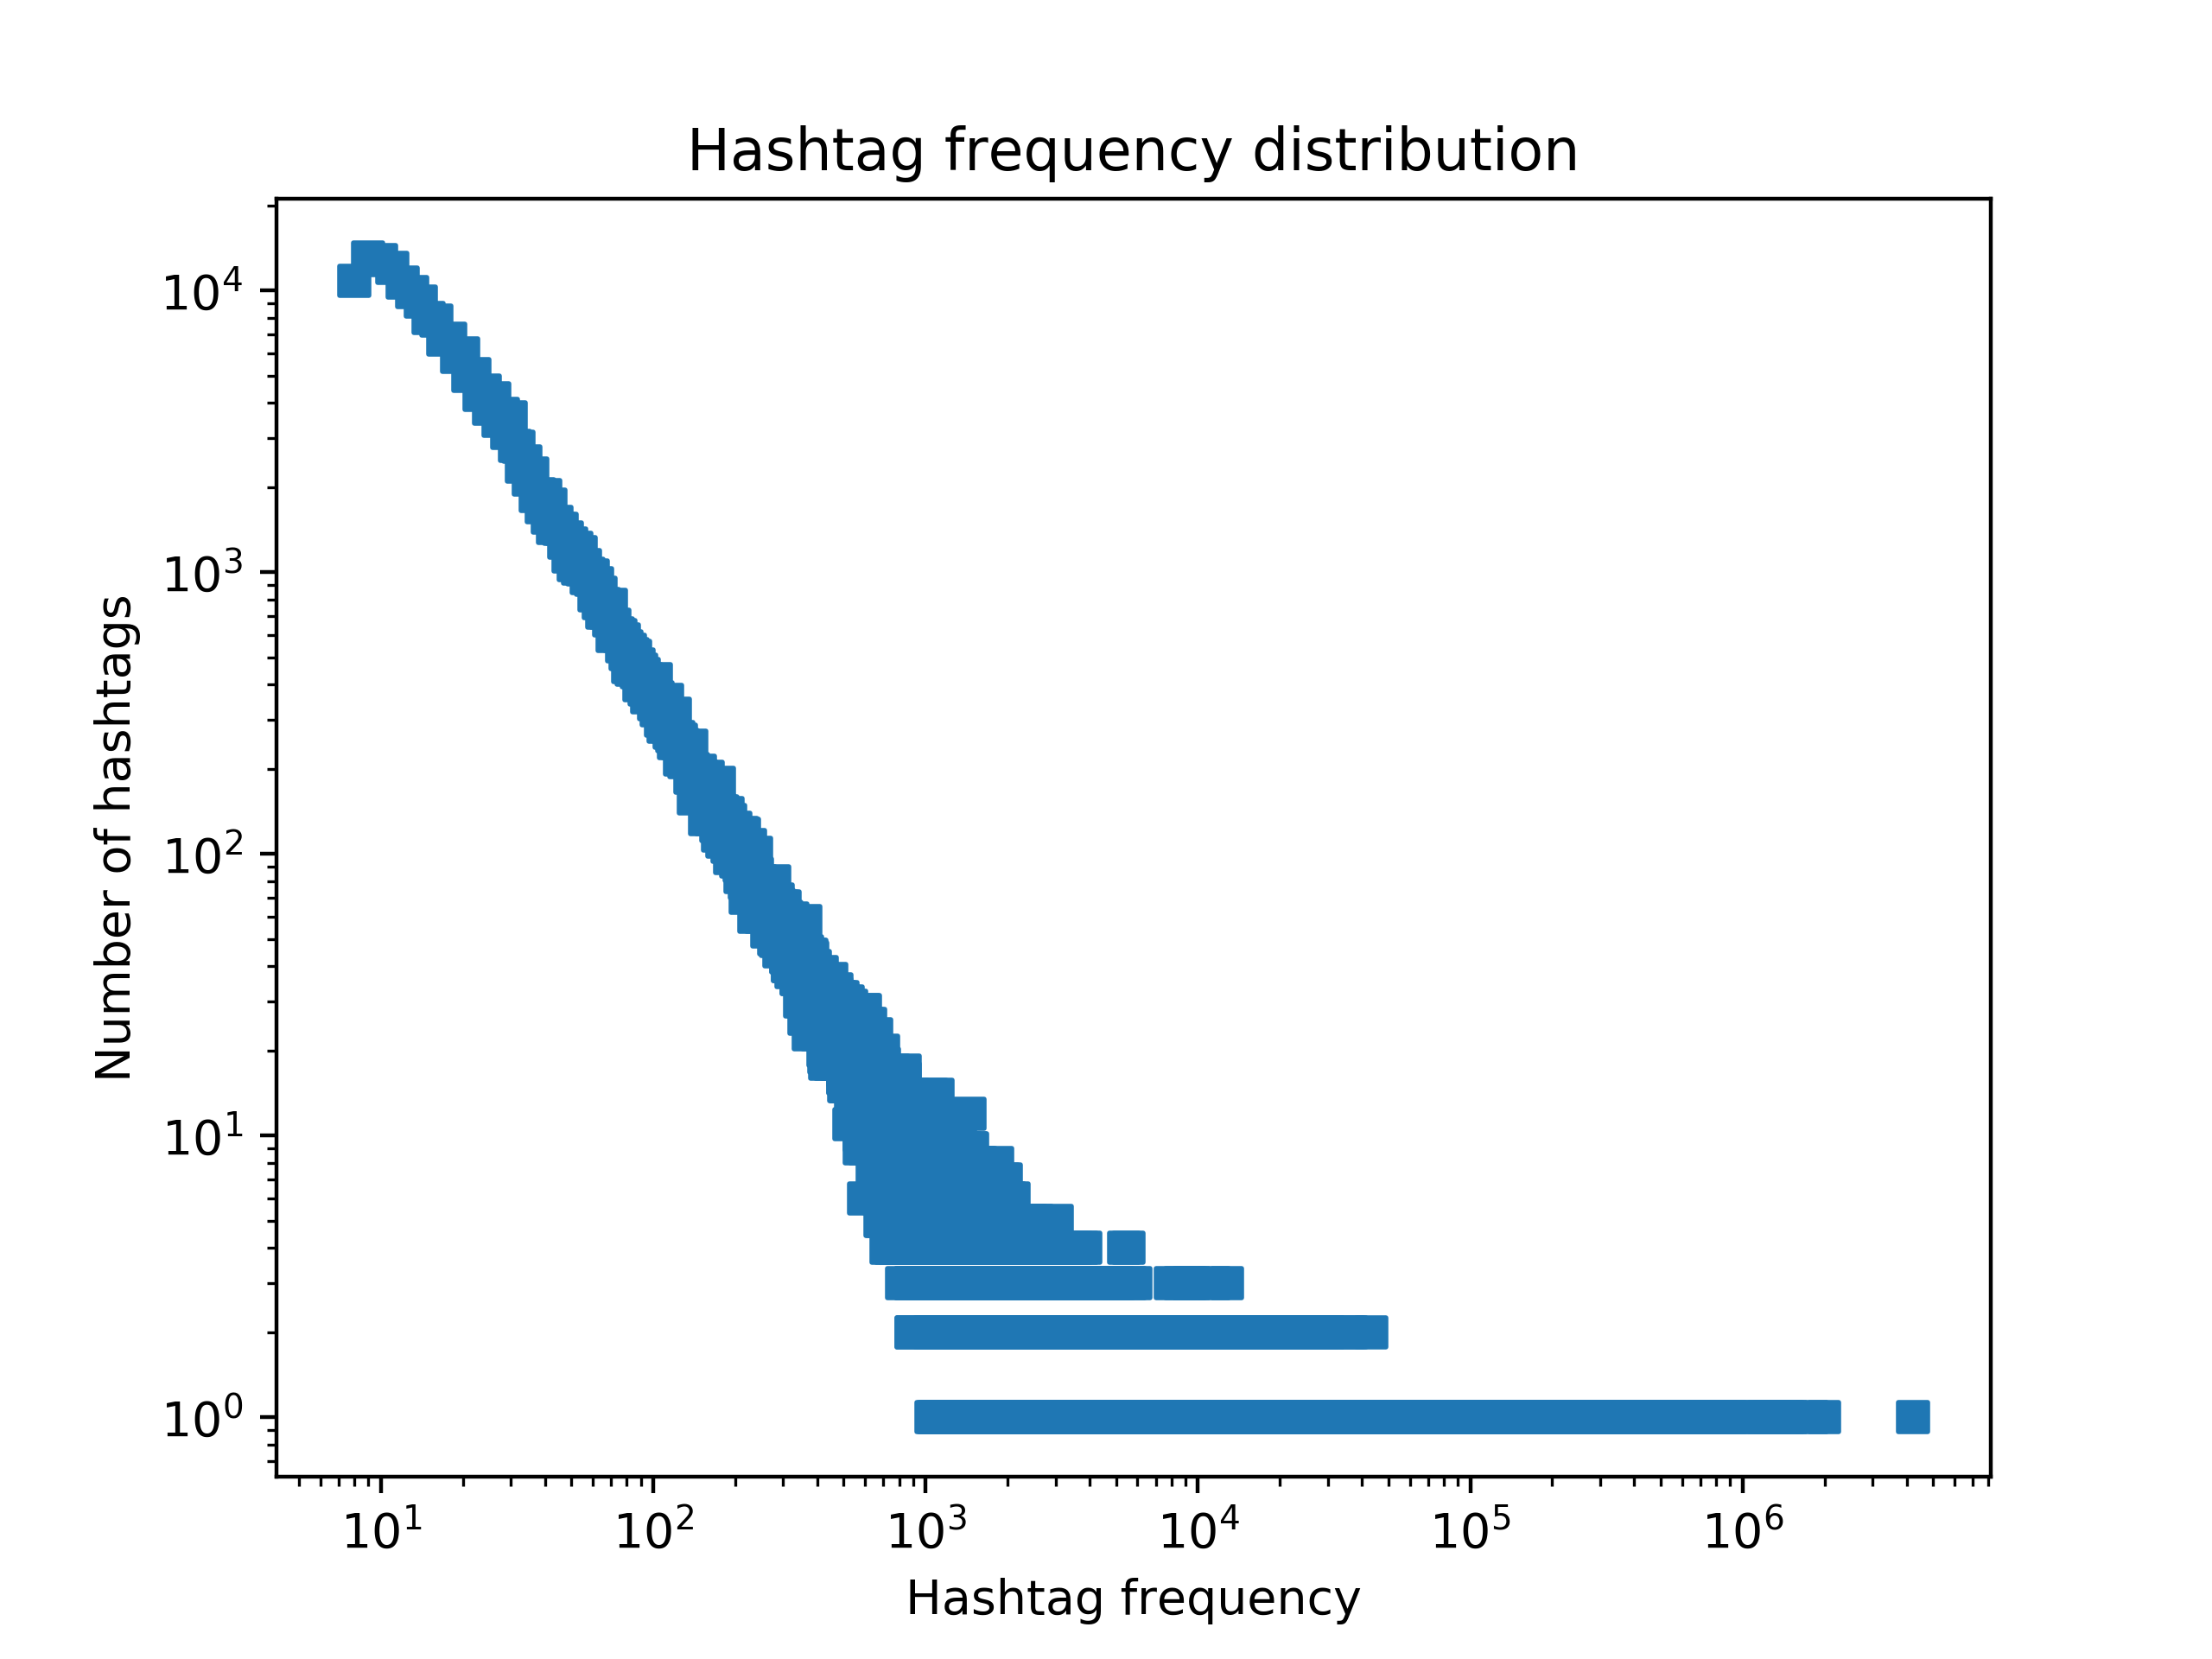
\includegraphics[width=0.5\textwidth]{hashtag_5}
    \bicaption{Hashtag频率分布}{Hashtag Frequency Distribution}
    \label{fig:g}
\end{figure}


目前 Hashtag 流行度预测的方法主要集中在研究其特有特征以及微博消息 的不同类型的特征,根据其不同特征,进行机器学习模型的优化。例如在前期的 研究中,Zongyang Ma 等人\citep{Ma2013On}在判断一个 Hashtag 是否会流行,考虑了内容特 征以及上下文特征,具体特征如表\ref{tab:hashtag-feature}所示。Oren Tsur 等人 \citep{tsur2012s}在预测 Hashtag 的流行度时,考虑了四中主要特征,包括 Hashtag 的内容,全局特征,图特征, 以及时间序列特征,论证了不同特征在模型中的重要性。但是目前的基于特征的 方法没有分析用户粉丝之间的网络结构特征以及对于 Hashtag 自身的特性挖掘 较少,模型的效果还有很大提升空间;另一方面,在刻画 Hashtag 主题标签内部 传播机制方面还没有研究,并且 Hashtag 是多源头的,不同的用户可以在不同的 时刻不断产生和转发,不同于传统的单源头消息预测,因此如何刻画多源头的主 题标签传播机制是一个研究的方向。

\begin{table}[!htbp]

    \bicaption{Hashtag特征}{Hashtag Feature}
    \label{tab:hashtag-feature}
    \centering
    \footnotesize% fontsize
    \setlength{\tabcolsep}{4pt}% column separation
    \renewcommand{\arraystretch}{1.2}%row space 
    \begin{tabular}{|l|l|}
        \hline
        \textbf{Type} & \textbf{Description}\\
        %\cline{2-9}% partial hline from column i to column j
        \hline
        \multirow{6}{*}{\textbf{Content Feature}}& number of tweets in Tth\\
&fraction of tweets containing URL\\
&fraction of retweet\\
&fraction of tweets with mention"@"\\
&hashtag clarity\\
&20-dimension hashtag topic vector\\ \hline

\multirow{8}{*}{\textbf{Context Feature}}
&number of users |Uth|\\
&average authority of users\\
&density of Gth\\
&fraction of users forming triangles in Gth\\
&ratio between the number of connected components and the number of nodes in Gth\\
&average edge weights in Gth\\
&number of border users\\
&15-dimension exposure probability vector\\ \hline
    \end{tabular}
\end{table}

\section{本章小结}
本章对传统消息流行度预测的方法以及 Hashtag 的流行度预测方法的相关研究工作进行了总结,并介绍了消息表示学习的研究进展,为后文基于用户粉丝网络结构特征的主题标签流行度预测算法和基于深度神经网络的多源头主题标 签流行度预测方法提供了理论基础。在传统的消息流行度预测方法上,主要还是 采用机器学习的方法,深度挖掘消息传播过程中的有效特征,该方法在实际应用 中效果较好,但是没有考虑 Hashtag 自身的情感性、地域性和事件性等特征以及 用户网络结构特征,因此本文在此方面考虑 Hashtag 的自身特性以及用户网络结 构特征,提出新的有效特征。另一方面目前深度学习在很多方面有了成功应用, 并且在消息预测上有了初步尝试,为后续多源头主题标签流行度预测提供了新 的思路。
\chapter{基于多维度特征的主题标签流行度预测}\label{chap:three}

在第二章中,我们介绍了当前消息流行度预测的常见方法以及 Hashtag 的流 行度预测方法,各个模型对于流行度预测的关注点具有不同的特点。首先从宏观 视角理解影响 Hashtag 传播的主要因素,建模 Hashtag 流行度预测模型。
前文已经分析了目前 Hashtag 流行度预测所使用的方法,主要是基于特征 的方法,然后使用机器学习模型进行训练预测,特征主要是内容特征,时间序 列等特征。但是目前已有的特征没有考虑用户粉丝之间的网络结构特征。在对 Hashtag 进行流行度预测时,因为消息是在用户粉丝网络结构上的传播,实质是 用户粉丝网络结构上的不断采样,因此考虑用户粉丝网络结构特征对于 Hashtag 流行度预测具有一定的价值。同时,Hashtag 产生以后,随着时间的迁移,虽然 是同一个 Hashtag,但是不同用户对其会有新的解读,因此考虑其动态的主题变 化,对于预测也会有一定的作用,并且不同的 Hashtag 所描述的主题可能具有明 显的地域色彩,因此抽取地域特征,将 Hashtag 进行地域分组,对于有效刻画不 同 Hashtag 的流行度预测有一定的帮助。

因此,在本章中,针对提高 Hashtag 流行度预测性能的目标,提出了基于利 用户粉丝网络结构特征,以及针对 Hashtag 的地域性,情感性等特征,采用机器 学习模型,进行 Hashtag 流行度预测,并通过实验验证了所提出特征的有效性。 本章的组织结构如下:首先介绍模型的基本思路;然后介绍模型训练与学习的具 体方法与步骤,本章中基于用户粉丝网络结构的向量学习将以 LINE 为基础,以 及 Hashtag 的情感性特征,基于 NMF 和 LDA 的微博的主题特征和进行分区域 的地域性特征。而其主要可以分为两个步骤:一是对用户粉丝网络结构数据以及 微博数据进行预处理,二是在对应的模型结构下完成特征的抽取, 特征和所用数 据如表\ref{tab:feature_data}所示。最后对本章提出的模型的有效性进行实验验证,实验结果表明, 本章所提出的特征能够提高 Hashtag 流行度预测的效果。

\begin{table}[!htbp]

    \bicaption{Hashtag特征和所用数据}{Hashtag Feature And Data}
    \label{tab:feature_data}
    \centering
    \footnotesize% fontsize
    \setlength{\tabcolsep}{20pt}% column separation
    \renewcommand{\arraystretch}{1.2}%row space 
    \begin{tabular}{cc}
        \hline
数据& 特征\\
        %\cline{2-9}% partial hline from column i to column j
        \hline
        \multirow{1}{*}{微博用户粉丝网络结构}& 基于 LINE 的用户向量表达 \\ \hline

\multirow{5}{*}{微博数据} &
时间序列特征 \\ &
内容特征\\&
Hashtag 自身特征 \\&
微博用户自身特征 \\&
微博消息特征\\
   
 \hline
    \end{tabular}
\end{table}



\section{Hashtag流行度的度量}

在研究如何预测 Hashtag 的流行度前,有必要对什么是 Hashtag 的流行度进
行定义。

所谓流行,即受欢迎。微博消息中的 Hashtag 的流行,意味着很多用户对该 Hashtag 进行转发或者原发,用户对此话题表示关注,受到他们的欢迎。在微博 消息中,一个 Hashtag 在一段时间内出现的次数代表这种受欢迎程度,如图\ref{fig:hashtag_popularity}所 示,不同 Hashtag 的阅读数不同,代表他们的受关注程度不同,因此流行程度也 不同。


\begin{figure}[!htbp]
    \centering
    \begin{subfigure}[b]{0.5\textwidth}
      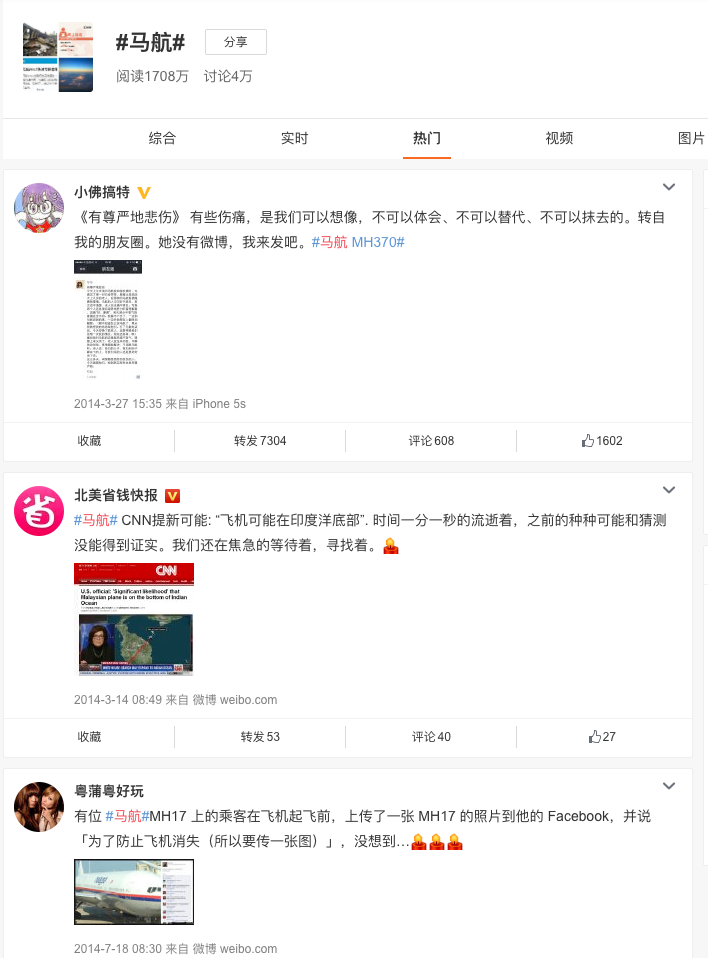
\includegraphics[width=\textwidth]{hashtag_popularity_a}

      \label{fig:hashtag_popularity_a}
    \end{subfigure}%
    ~%add desired spacing
    \begin{subfigure}[b]{0.5\textwidth}
      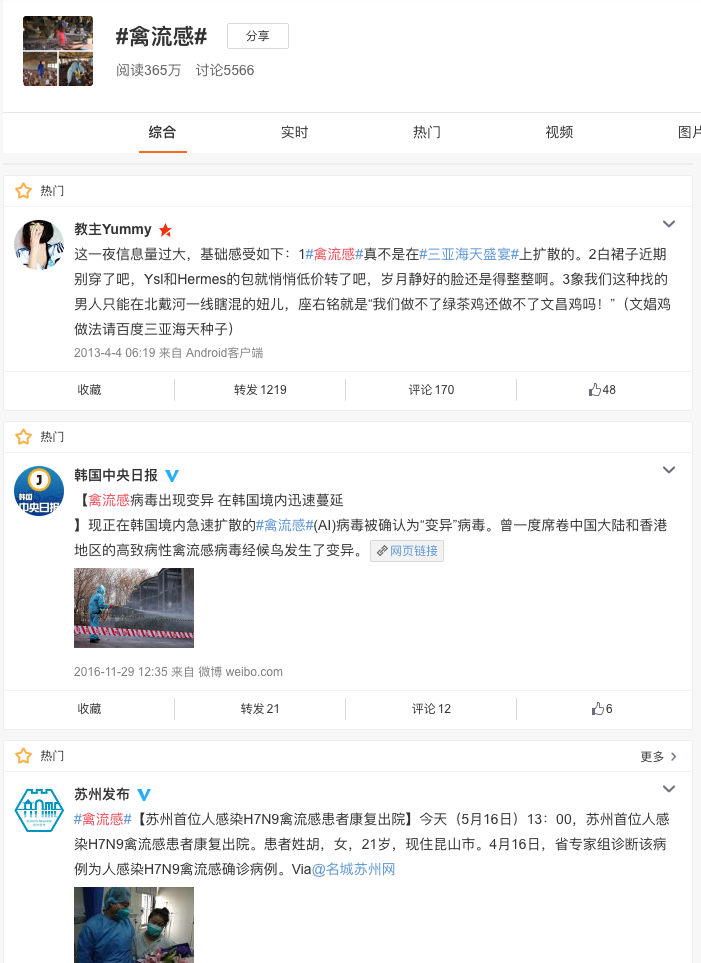
\includegraphics[width=\textwidth]{hashtag_popularity_b}

      \label{fig:hashtag_popularity_b}
    \end{subfigure}
    \bicaption{不同 Hashtag 的阅读数以及出现情况}{Readings And Occurrences Of Different Hashtag}
    \label{fig:hashtag_popularity}
\end{figure}
在本文中,使用 Hashtag 在微博消息中出现的次数来表示该 Hashtag 的流行 度,原因如下:\begin{enumerate}
\item 当用户在一条微博消息中添加 Hashtag 的时候,表示用户对此 Hashtag 的 认可,这个操作真实的表达了用户的主观意见;
\item 是否为热点话题是一个二值化的属性,即“是”与“不是”,可以对应“流行” 与“不流行”,但是不能完整的体现“度”的概念,而出现的次数是一个数值化的属 性,则能更好地表现流行的“程度”;
\end{enumerate}

因此,本文使用 Hashtag 在微博中出现的次数来代表其流行度,进行预测。

\section{问题描述和基本思路}

\subsection{问题描述}

本章所要研究的主要是根据历史上 Hashtag 出现的情况,预测未来某时刻内 Hashtag 出现的频率,具体是根据 Hashtag 过去连续两周的数据预测接下来一天 内 Hashtag 出现的次数,模型预测的结果要尽量和真实数值接近,Hashtag 出现 次数时间分布如图\ref{fig:3_1}所示,由图可知大部分的 Hashtag 的存活时间是超过两周 的,因此该预测问题是有效的。

\begin{figure}[H]
    \centering
    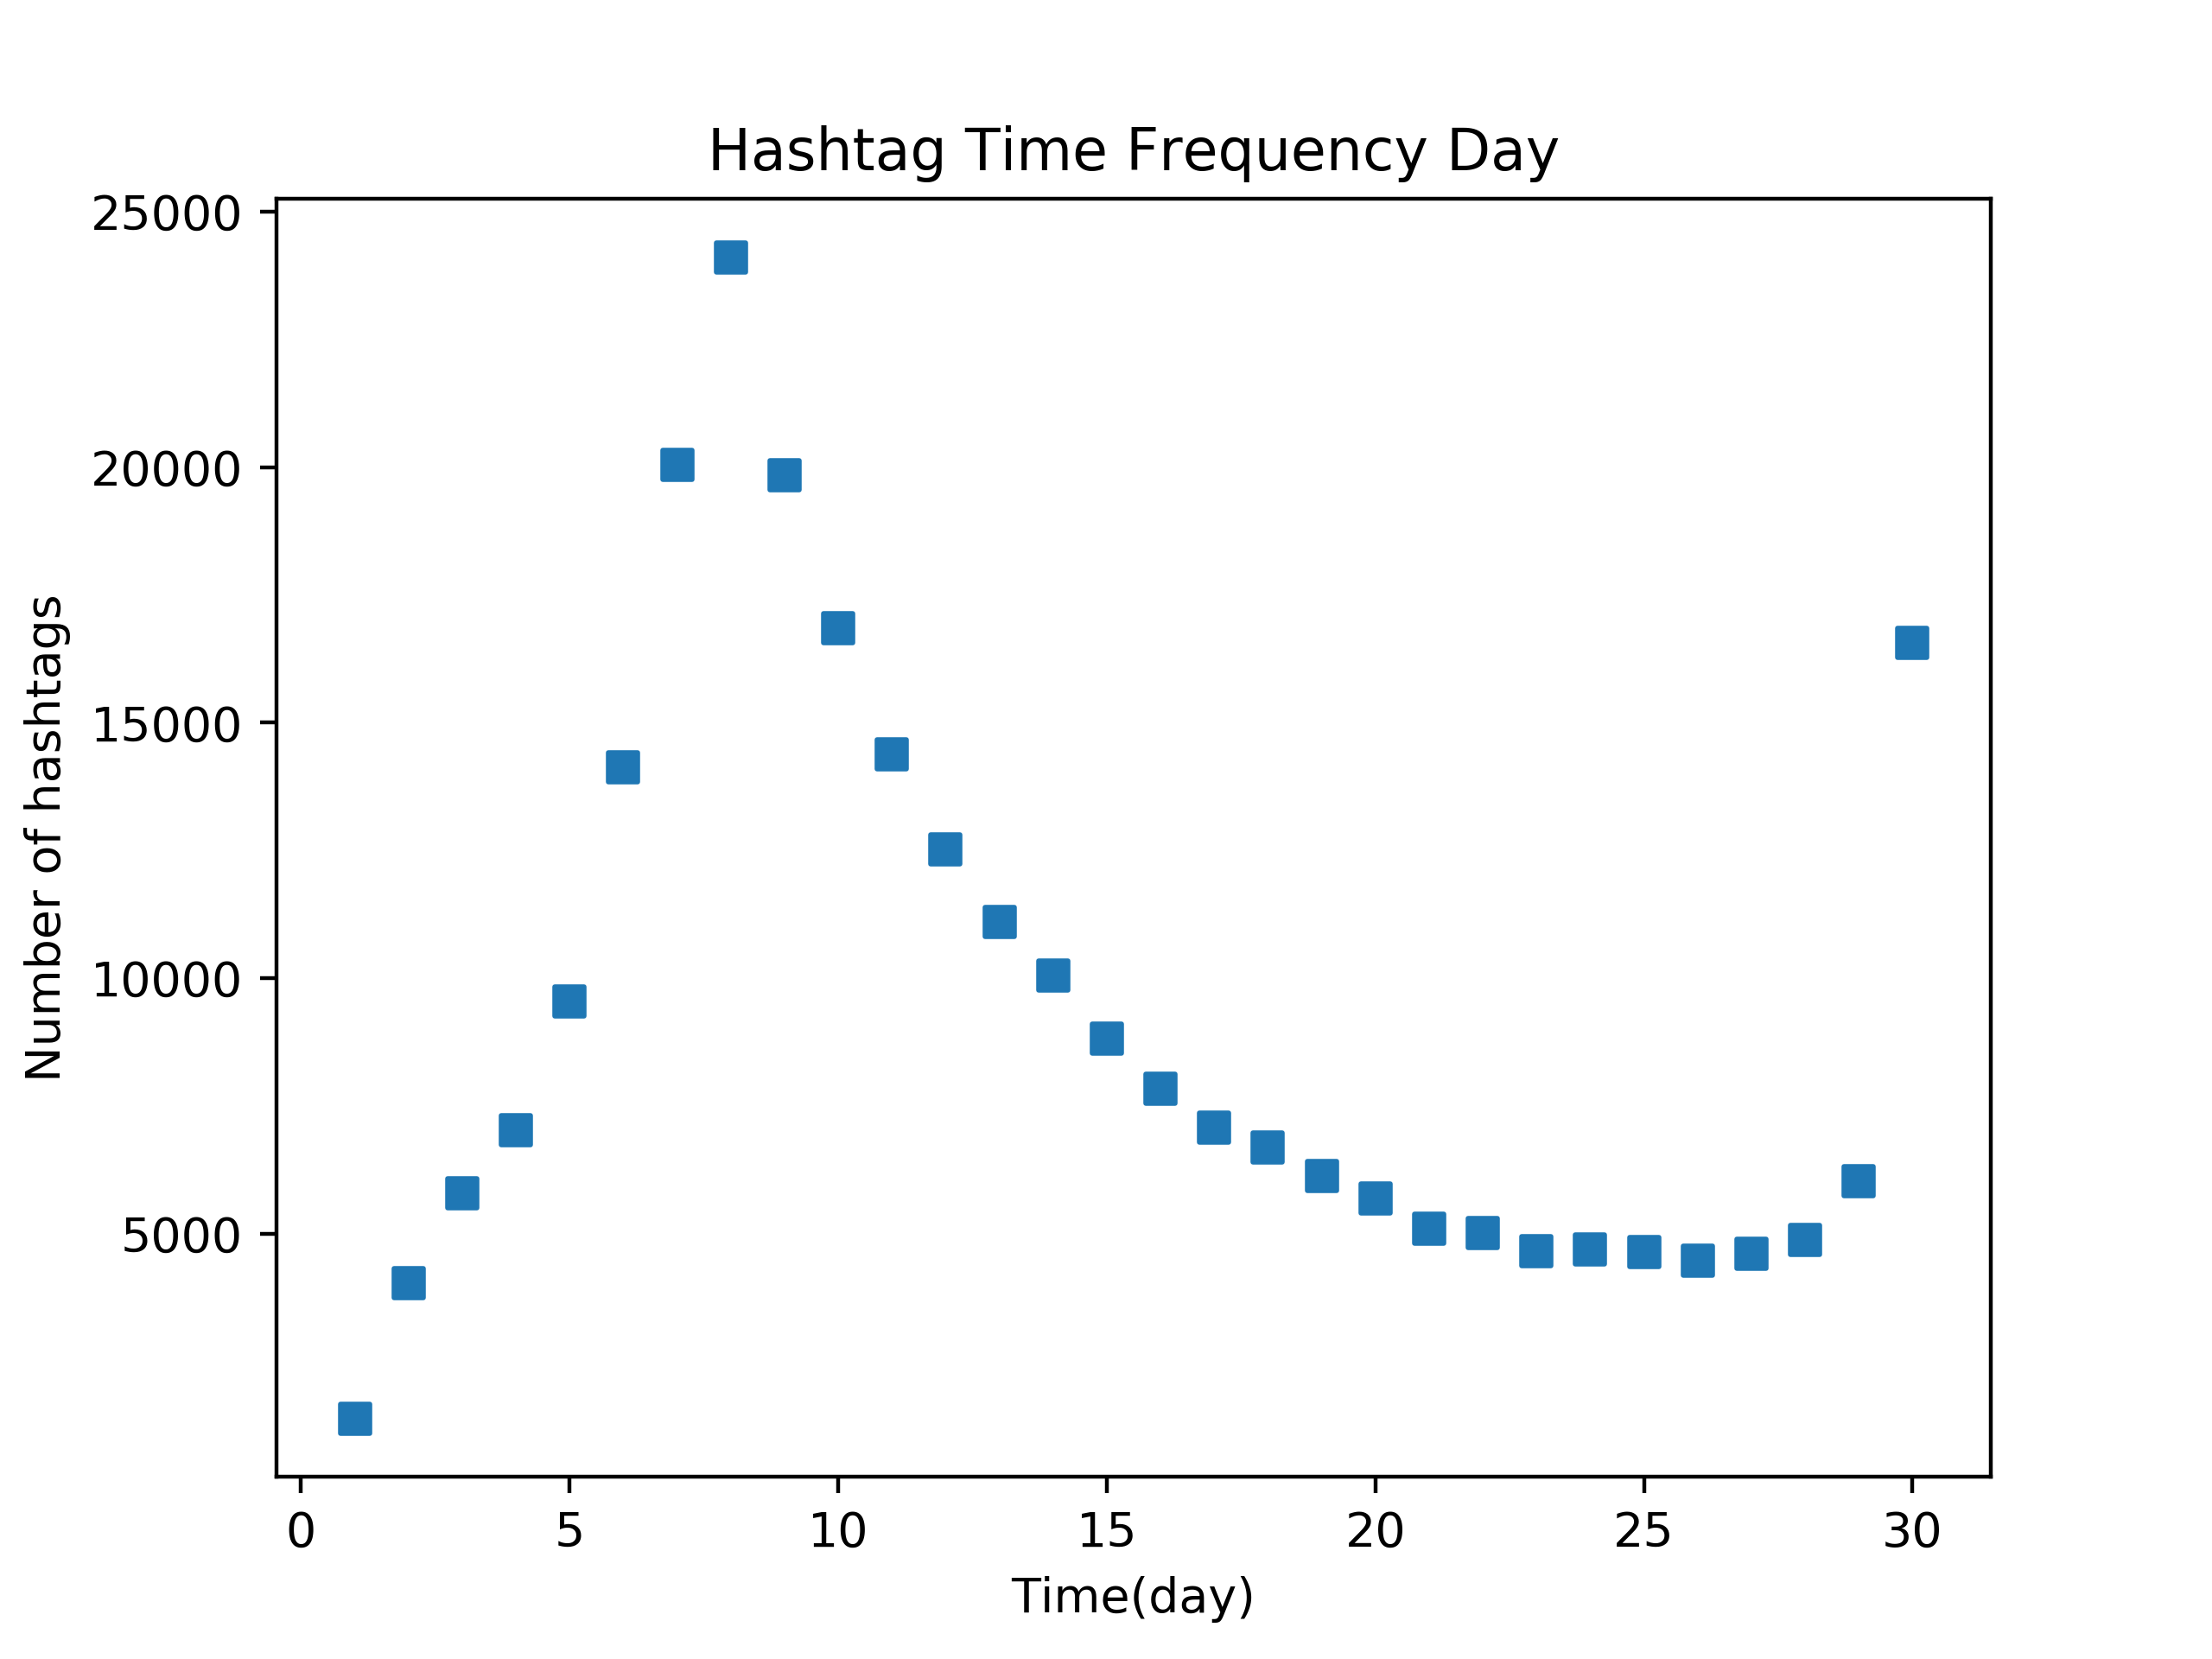
\includegraphics[width=0.5\textwidth]{hashtag_time_new_1}
    \bicaption{Hashtag 时间次数分布图}{Hashtag Time Distribution Chart}
    \label{fig:3_1}
\end{figure}

\subsection{基本思路}
现有的社交网络中的 Hashtag 流行度预测问题没有考虑用户之间的社交网络 结构以及 Hashtag 自身的特性。当前的流行度预测问题,主要考虑的是 Hashtag 的时间序列特征以及 Hashtag 的内容特征,例如考虑时间间隔内 Hashtag 的转发 次数,来预测接下来的转发情况,当然时间序列特征是一个直观并且比较有效的 特征,它很好的反映了消息一个时间段内的热门程度。但是 Hashtag 本身是由用 户产生并且进行转发的,用户之间的关注关系是十分重要。并且 Hashtag 有其自 身特性,比如情感性,地域性以及事件性,这些都是其自身重要的特征,对于预 测 Hashtag 的流行度具有很大作用。因此,本文希望在现有的特征的基础上考虑 用户的粉丝网络结构特征以及 Hashtag 的自身特性,更好的进行 Hashtag 流行度 预测。

因此,本章的基本思路是考虑原有的时间序列等特征,结合用户的粉丝网络 结构特征,学习每个用户的向量表示,刻画用户特征。同时考虑 Hashtag 自身特 性,考虑其情感性以及地域性,构建 Hashtag 不同消息的重要特征。在此特征的 基础上,采用多种机器学习模型,进行 Hashtag 流行度预测的实验。

由于本章所使用的特征涉及用户粉丝网络结构表示以及主题模型,所以首 先对这两部分的内容进行说明,便于后续特征工程的展开。

\section{⺴络表示学习}
网络表示学习(Representation Learning on Network),通常来说就是网络的
向量化技术,简单来说,即将网络中的结构(节点、边或者子图),通过一系列
 过程,变成一个多维向量,通过这样的操作,能够将复杂的网络结构信息变成结 构化的多维特征,实现可计算的向量表示,从而利用机器学习方法实现更方便的 算法应用。

\subsection{基于 DeepWalk 的用户粉丝网络表示}

Deepwalk 是 2014 年发表在 KDD 上的一篇论文 \citep{Perozzi2014DeepWalk},这篇文章受到了词向量 学习模型 word2vec 的启发,文章的思路就是对网络应用了 word2vec 的 SkipGram 模型。SkipGram 模型原本是针对文本数据进行学习的,或者说是针对有序序列 的,因此 Deepwalk 先应用随机游走得到网络中的一些列有序的节点序列,这些 节点序列类似于文本中的句子,通过这样的数据处理方式,将这些“句子”使用 SkipGram 模型进行训练,从而得到“句子”中每个“单词”的向量表示,结果数据展 示如图\ref{fig:piu_0}所示。
\begin{figure}[!htbp]
    \centering
    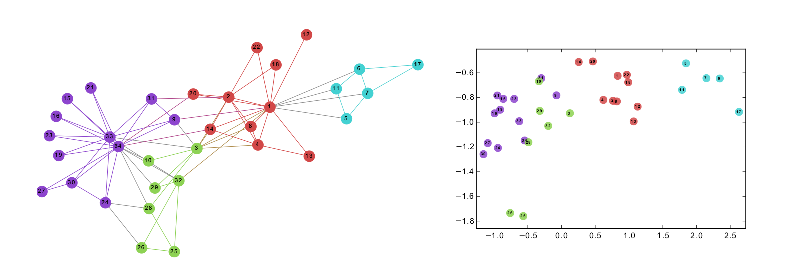
\includegraphics[width=0.7\textwidth]{dw}
    \bicaption{DeepWalk 数据展示 \citep{Perozzi2014DeepWalk}}{DeepWalk Show\citep{Perozzi2014DeepWalk}}
    \label{fig:piu_0}
\end{figure}


Deepwalk 的随机游走过程事实上是对网络结构进行随机采样的过程,将网 络中的节点通过随机游走的方式表示出来,两个节点联系越紧密,在一个随机游 走过程中共同出现的可能性越大,反之若两个节点根本不连通,则随机游走的方 式是不可能将两个节点共同出现的。因此 Deepwalk 能很好的将网络的连接情况 进行表示,且实验证明在网络规模较大时具有很高的效率,其算法流程如\ref{alg:DeepWalk_1}和\ref{alg:SkipGram_1}。

\begin{algorithm}[H]
\renewcommand{\algorithmicrequire}{\textbf{Input:}} 
\renewcommand{\algorithmicensure}{\textbf{Output:}}
    \small
    \caption{DeepWalk(G,$\omega$,d,$\gamma$,t)}
    \label{alg:DeepWalk_1}
    \begin{algorithmic}
    \Require graph G(V,E) \\
    window size $\omega$ \\ 
    embedding size d \\
     walks per vertex $\gamma$ \\ 
     walk length t 
     \Ensure{matrix of vertex representations $\Phi$ $\in$  $R^{|V|{\times}d}$}
     
      \State $ Initialization: Sample ~\Phi from U^{|V |d}$
      \State $Build~ a~ binary ~Tree~ T ~from~ V $
       \For {i~=~0 to $\gamma$} 
			\State $O = Shuffle(V ) $
			\For  {${v_i}$~ $\in$~O}
				\State $W_{v_i} = RandomWalk(G,v_i,t)$
				\State $SkipGram(\Phi, W_{v_i} , w)$
			\EndFor
		\EndFor
    \end{algorithmic}
\end{algorithm}

\begin{algorithm}[H]
    \small
    \caption{SkipGram($\Phi$,$\Omega_{v_i}$,$\omega$)}\label{alg:SkipGram_1}
    \begin{algorithmic}[1]
       \For {${v_j}$ $\in$ $\Omega$} 
			\For  {${u_k}$~ $\in$~$\Omega_{v_i}[j - w : j + w]$}
				\State $J(\Phi) = -\log Pr(u_k|\Phi(v_j))$
				\State $\Phi = \Phi - \alpha * \frac{\partial J}{\partial \Phi}$
			\EndFor
		\EndFor
    \end{algorithmic}
\end{algorithm}

其大致思想就是用随机游走蒙特卡罗采样,然后送到 word2vec 去训练,最 终得到每个节点的向量表示,训练方式如图\ref{fig:piu_1}所示。


\begin{figure}[H]
    \centering
    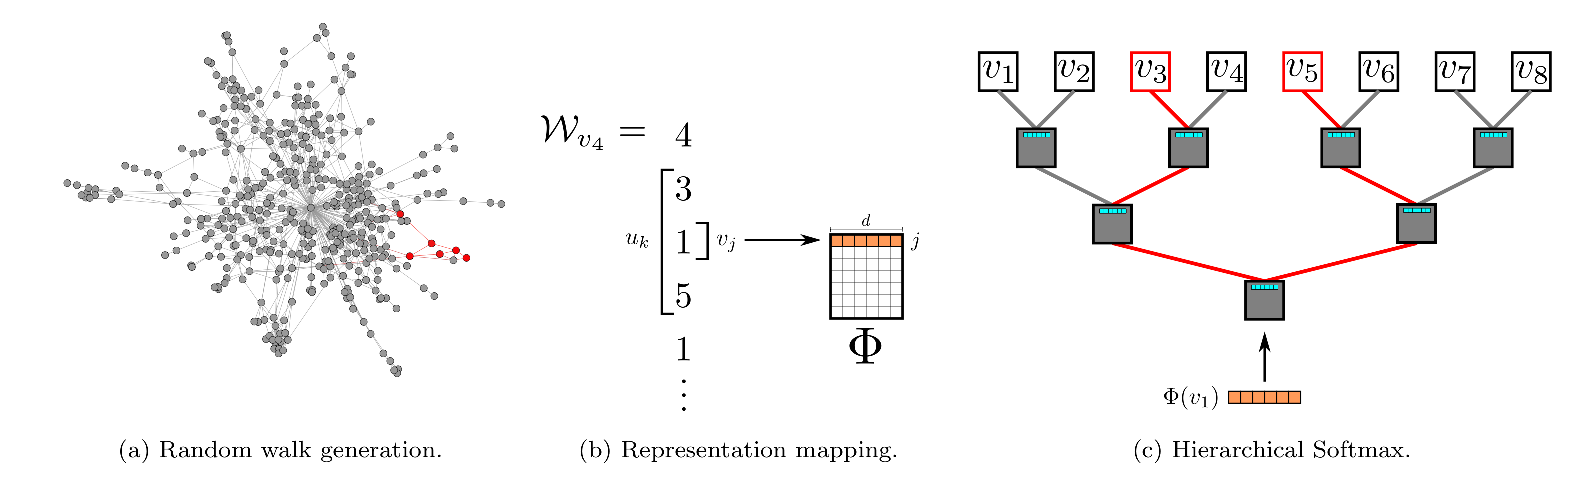
\includegraphics[width=0.7\textwidth]{hashtag_1}
    \bicaption{DeepWalk训练过程\citep{Perozzi2014DeepWalk}}{DeepWalk Training Process\citep{Perozzi2014DeepWalk}}
    \label{fig:piu_1}
\end{figure}

\subsection{基于 LINE 的用户粉丝网络表示}
LINE 是 2015 年提出的一种网络结构表示学习方法,该方法提出了一阶邻 近度与二阶邻近度的概念,基于这两个邻近度,提出了优化函数,得到的最优化 结果即为每个节点的向量表示\citep{Tang2015LINE}。

该方法的优化过程可以理解为基于两个假设:
\begin{enumerate}


\item 直接相连的节点表示尽可能相近(一阶邻近度),它们的距离尽可能的 小,如图\ref{fig:piu_2}中的节点 6 和节点 7。文中两个节点的联合概率表示其一阶邻近度, v 代表节点,u 代表节点的 embedding。公式\ref{eq:line_1}的意思是两节点越相似,内积越 大,sigmoid 映射后的值越大,也就是这两节点相连的权重越大,也就是这两个 节点间出现的概率越大。

\begin{equation}\label{eq:line_1}
	p_1(v_i,v_j) = \frac{1}{1 + \exp(-\overrightarrow{u_i}^{T} ~\cdot~ \overrightarrow{u_j})}
\end{equation}

\item 两个节点公共的邻居节点越多,两个节点的表示越相近(二阶邻近度),
如图\ref{fig:piu_2}中的节点 5 和节点 6。公式\ref{eq:line_2}用两个节点的条件概率表示其二阶邻近度。

\begin{equation}\label{eq:line_2}
	p_2(v_i|v_j) = \frac{\exp(\overrightarrow{u_j}^{\prime T}~\cdot~\overrightarrow{u_i})}{\begin{matrix}
	\sum_{k=1}^V ~\exp(-\overrightarrow{u_k}^{\prime T} ~\cdot~ \overrightarrow{u_j})
\end{matrix}	 }
\end{equation}


\end{enumerate}

\begin{figure}[H]
    \centering
    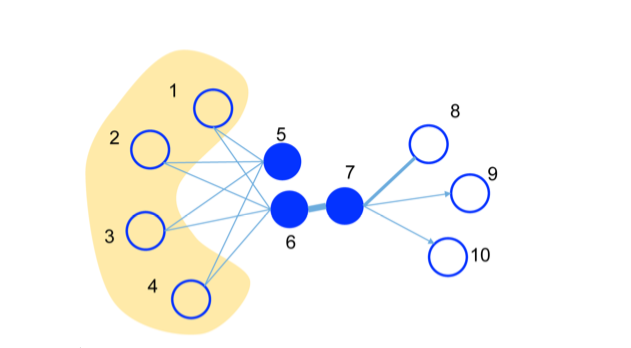
\includegraphics[width=0.7\textwidth]{hashtag_}
    \bicaption{用户网络结构图\citep{Tang2015LINE}}{User Network Structure\citep{Tang2015LINE}}
    \label{fig:piu_2}
\end{figure}

\subsection{小结}
对比网络表示学习中的 DeepWalk 和 LINE 等算法的原理,考虑到 LINE 算
法提出了一个明确的目标函数,问题可以进行直接优化,对于网络表示学习有更
 好的结果,因此本文的用户粉丝网络结构表达采用 LINE 的方式进行学习,通过 明确的优化方式,用户的向量表达更加准确。

\section{主题模型}
在人们日常获取信息的方式上,文本占有很大分量,为了更快更精确地从大 量的文本数据中取得所需要的信息,针对文本信息处理的研究一直在进行。文本 数据不光信息量大,而且一般是无结构的。另外,通常的文本数据以矩阵的形式 被计算机处理,此时的数据矩阵具有高维稀疏的特征,空间占用较大,因此,对 大规模文本信息进行处理分析的另一个障碍便是如何削减原始数据的维度。


\subsection{NMF 非负矩阵分解}
通常的矩阵分解会把一个大的矩阵分解为多个小的矩阵,但是这些矩阵的 元素有正有负。而在现实世界中,文本数据等形成的矩阵中负数的存在是没有 意义的,因此如果能把一个矩阵分解成全是非负元素的矩阵是很有价值的。在 NMF 中要求原始矩阵中的所有元素均是非负的,那么矩阵可以分解为两个更小 的非负矩阵的乘积,这个矩阵有且仅有一个这样的分解,即满足存在性和唯一性\citep{Du2010Nonnegative}。

NMF 的思想:V=WH(W 权重矩阵、H 特征矩阵、V 原矩阵),通过计算从 原矩阵提取权重和特征两个不同的矩阵出来,NMF 属于一个无监督学习的算法, 其中限制条件就是 W 和 H 中的所有元素都要大于等于 0。

\begin{figure}[H]
    \centering
    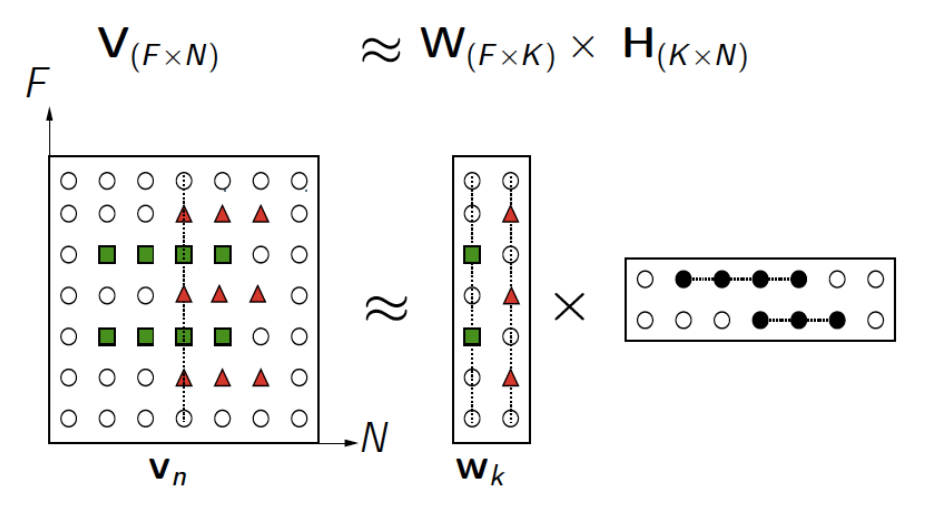
\includegraphics[width=0.5\textwidth]{hashtag_2}
    \bicaption{NMF矩阵分解示意图}{NMF Matrix Decomposition Diagram}
    \label{fig:piu_5}
\end{figure}

\subsection{LDA 主题模型}

LDA(Latent Dirichlet Allocation)是一种文档主题生成模型,也称为一个三层贝叶斯概率模型,包含词、主题和文档三层结构 \citep{Blei2003Latent}。所谓文档主题生成模型,
 就是认为一篇文章中的每个词都是通过“以一定概率选择了某个主题,并从这个 主题中以一定概率选择某个词语”这样一个过程得到的。文档到主题服从多项式 分布,主题到词服从多项式分布。
 
LDA 是一种非监督机器学习技术,可以用来识别大规模文档集(document collection)或语料库(corpus)中潜藏的主题信息。它采用了词袋模型(bag of words)的方法,这种方法将每一篇文档视为一个词频向量,从而将文本信息转 化为了易于建模的数字信息。词袋方法没有考虑词与词之间的顺序,这简化了问 题的复杂性,同时也为模型的改进提供了方向。每一篇文档代表了一些主题所构 成的一个概率分布,而每一个主题又代表了很多单词所构成的一个概率分布。

LDA 主题模型主要是对文档词矩阵进行降维,数据输入如图\ref{fig:piu_6}所示。

\begin{figure}[H]
    \centering
    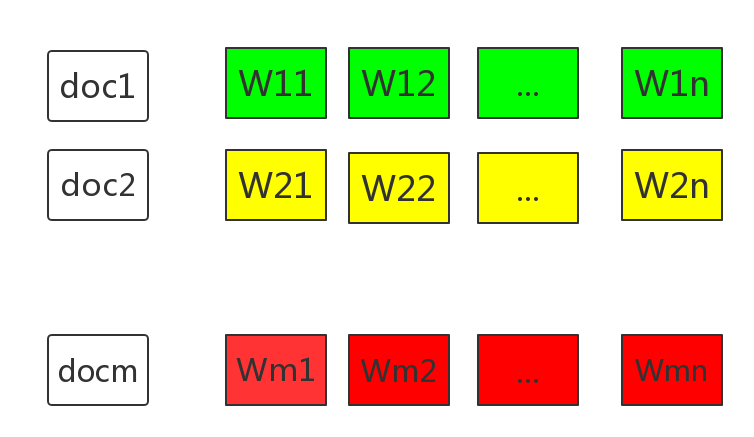
\includegraphics[width=0.5\textwidth]{lda}
    \bicaption{LDA文档词矩阵}{LDA Document Word Matrix}
    \label{fig:piu_6}
\end{figure}


LDA 模型的目标是找到每一篇文档的主题分布和每一个主题中词的分布。 在 LDA 模型中,我们需要先假定一个主题数目 K,这样所有的分布就都基于 K 个主题展开, 具体过程如图\ref{fig:piu_7}所示。
\begin{figure}[H]
    \centering
    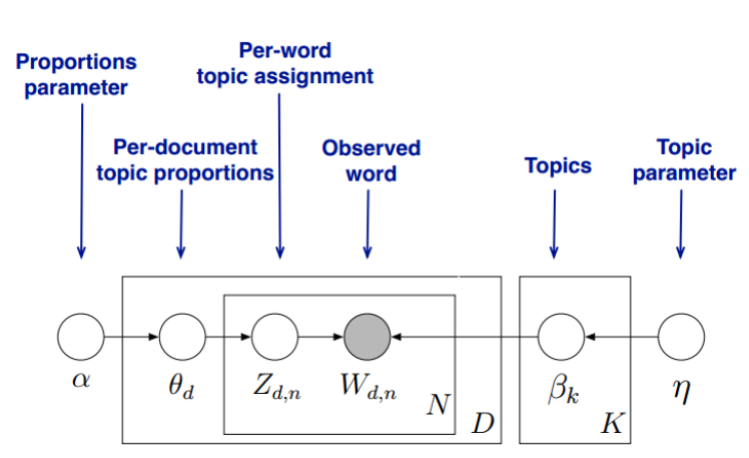
\includegraphics[width=0.5\textwidth]{hashtag_4}
    \bicaption{LDA主题模型流程图}{LDA Flow Chart}
    \label{fig:piu_7}
\end{figure}

\section{Hashtag数据特点}

如在相关研究中所述,在消息流行度预测领域有很多已有的研究成果,比 如对微博中热门话题的发现和预测等,其中的一些方法可以直接应用在本文所 要研究的问题上,但这些研究成果因为没有考虑到 Hashtag 流行度预测的场景特 点,都有提高的空间。

在进行 Hashtag 流行度预测之前,本文首先分析其出现频次的特征,从宏观 角度考察数据分布情况,对于后期特征的提取以及模型的优化有较大的指导意 义。

相比于微博消息的流行度预测,Hashtag 流行度预测与其存在一些共性,比 如它们的分布都是呈现幂律分布的,如图\ref{fig:piu_8}所示,因此消息预测中的一些特性, 比如时间序列特征很显然可以适用到 Hashtag 的流行度预测中。


\begin{figure}[H]
    \centering
    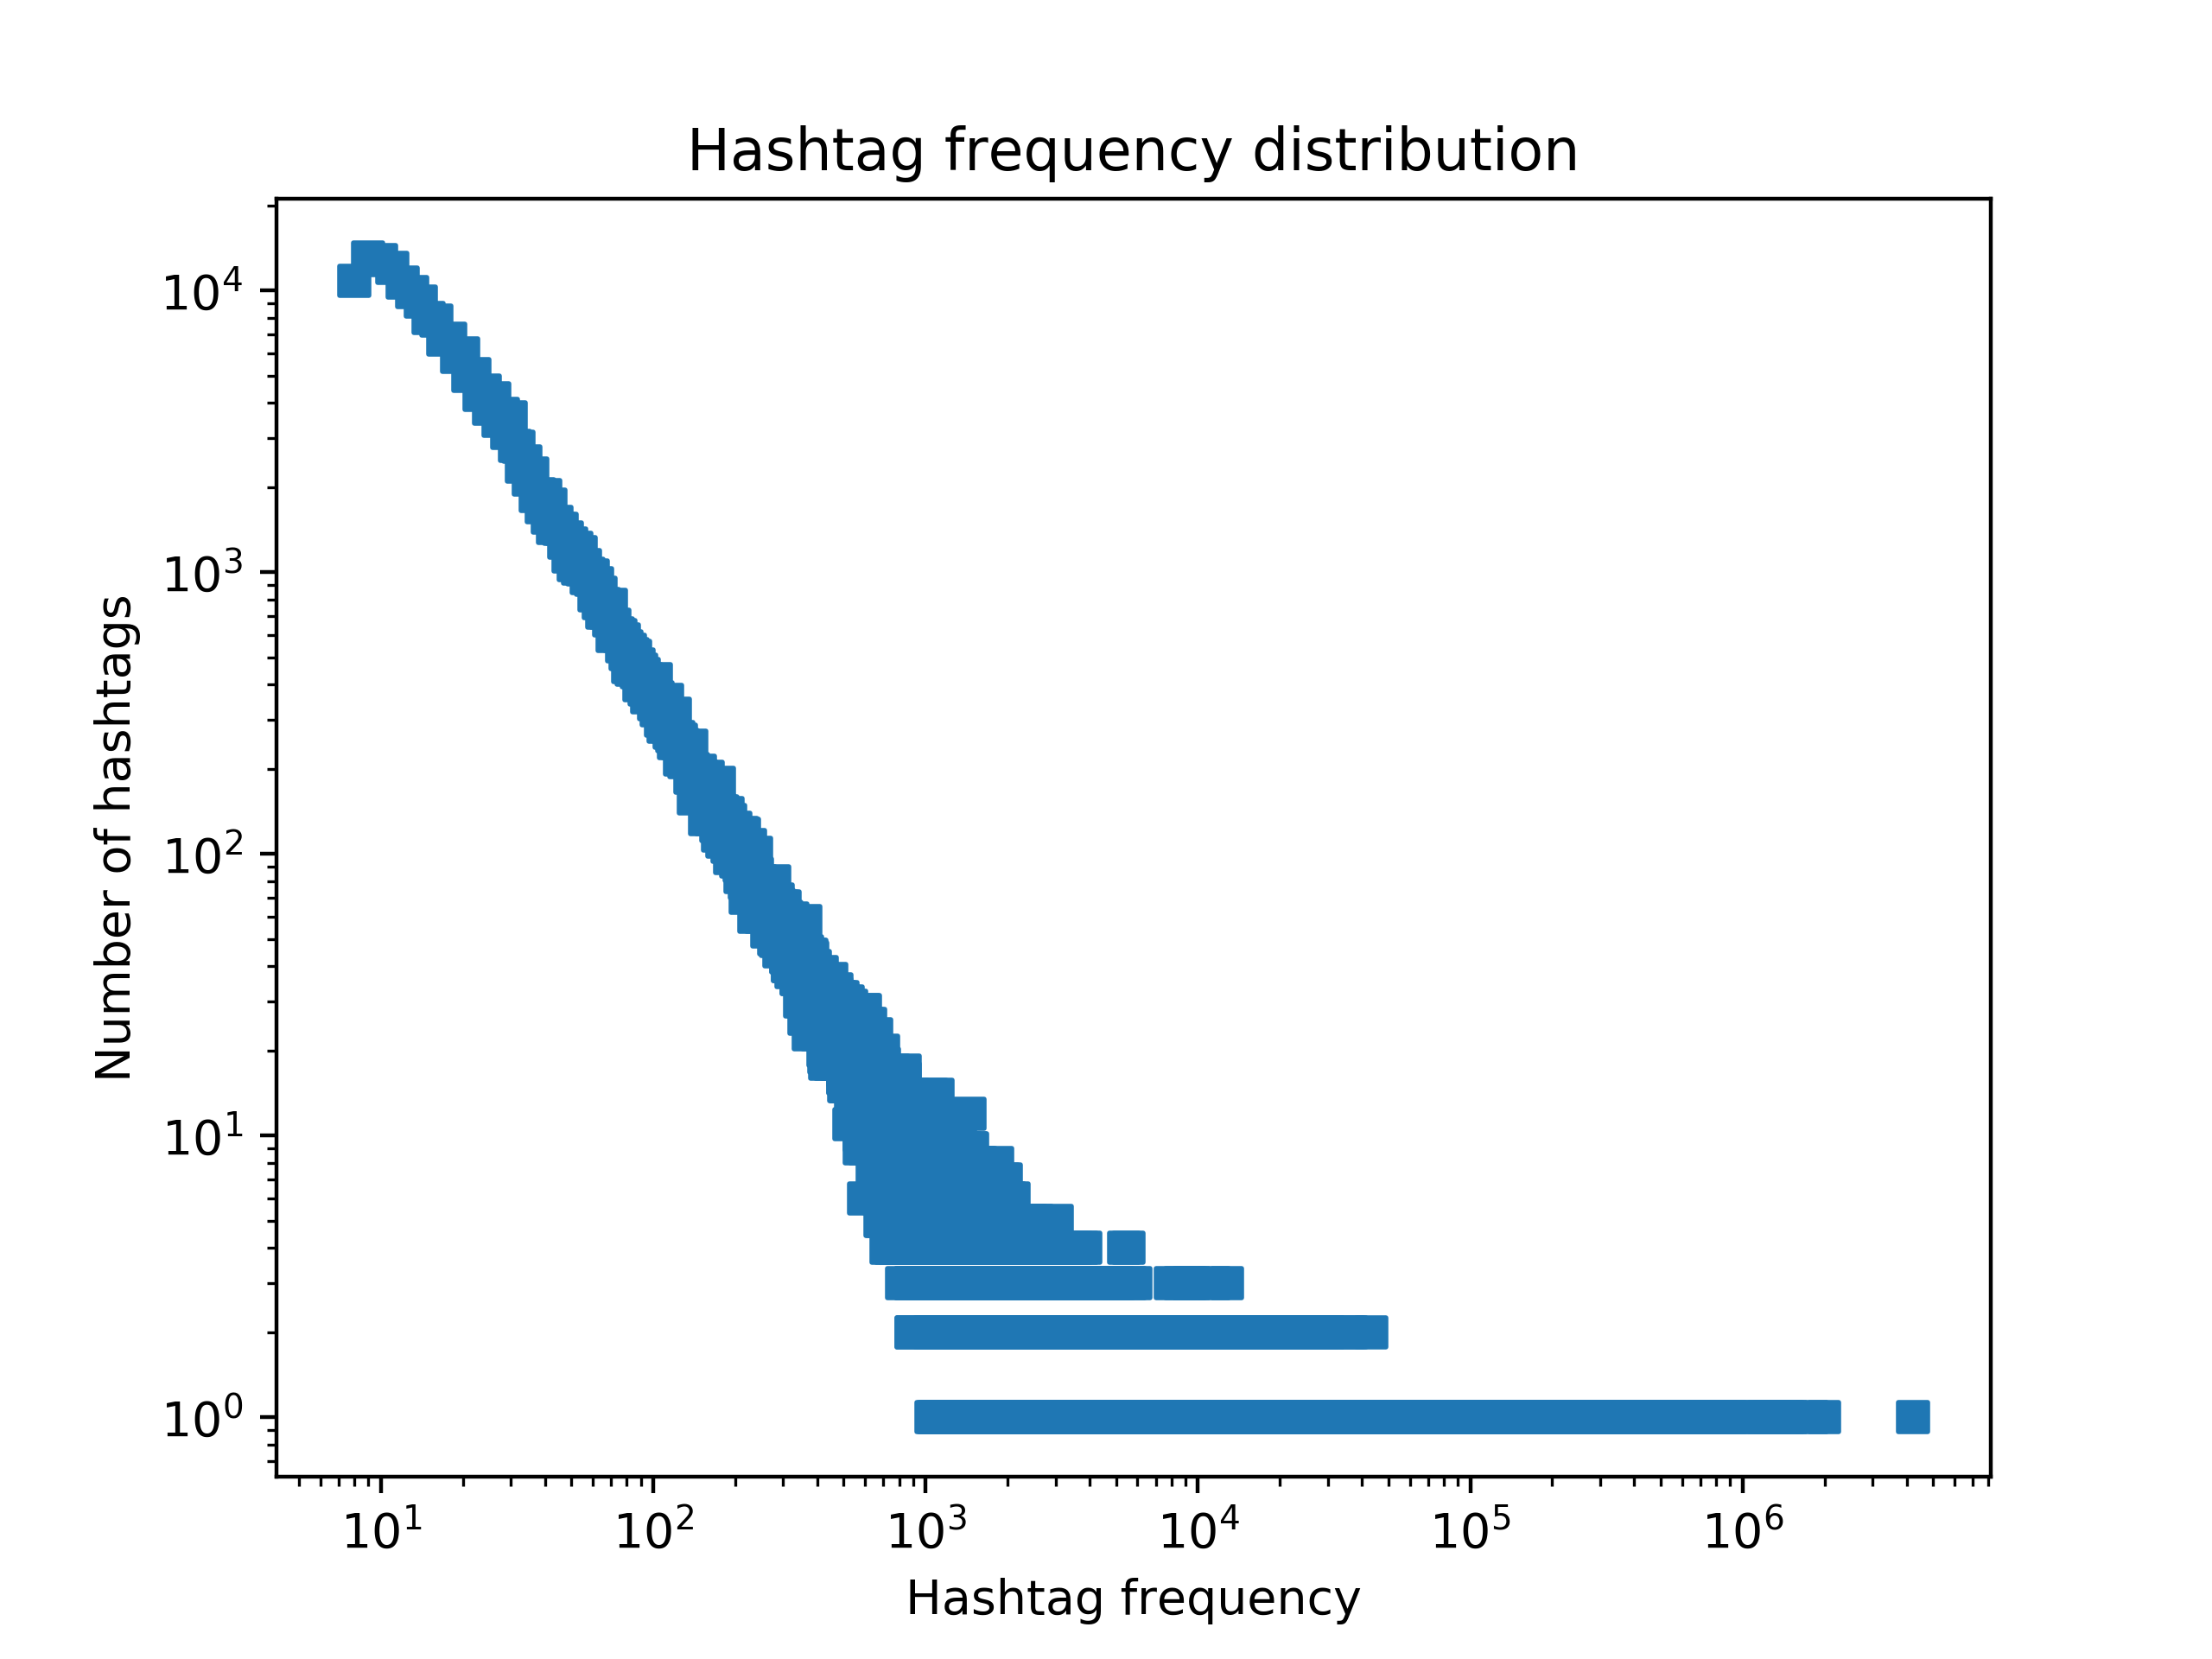
\includegraphics[width=0.5\textwidth]{hashtag_5}
    \bicaption{Hashtag分布情况}{Hashtag Distribution}
    \label{fig:piu_8}
\end{figure}


但是 Hashtag 自身存在许多消息不存在的特性,Hashtag 本身可以作为一个 事件或者一个话题,其带有鲜明的主观意愿,而微博消息本身对于事件的表述 不是很准确,无法从单一的微博消息获得深入的认识,而 Hashtag 短短几个字就 抓住了用户的想法,所以它们之间存在很大区别。比如对于 \# 李小璐出轨 \# 这个 Hashtag,如图\ref{fig:lixiaolu}所示,它的流行度预测受标签本身的特性影响很大,比如里面 出现的公众人物,情感色彩,地域信息等等,而这些在微博消息中都是很难捕捉 到的。


\begin{figure}[!htbp]
    \centering
    \begin{subfigure}[b]{0.5\textwidth}
      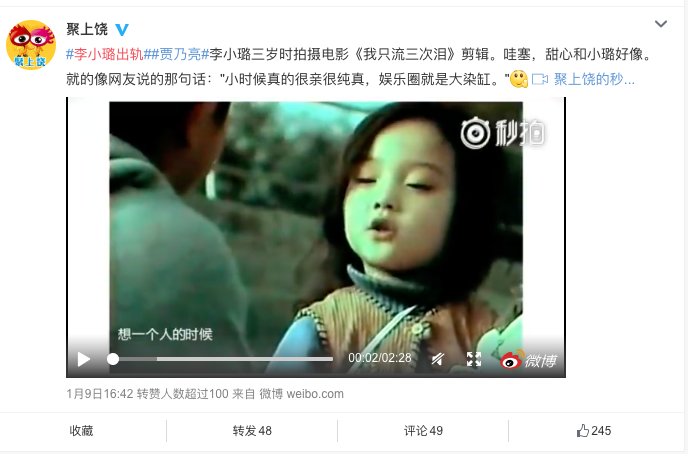
\includegraphics[width=\textwidth]{l_1}
      \caption{}
      \label{fig:oaspl_a}
    \end{subfigure}%
    ~%add desired spacing
    \begin{subfigure}[b]{0.5\textwidth}
      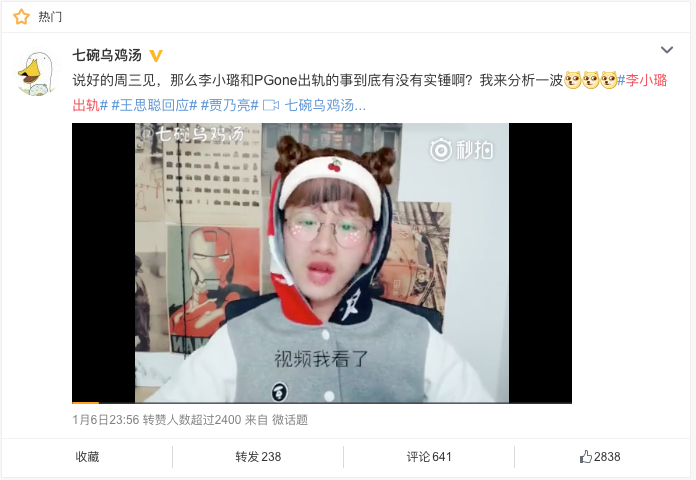
\includegraphics[width=\textwidth]{l_2}
      \caption{}
      \label{fig:oaspl_b}
    \end{subfigure}
    \begin{subfigure}[b]{1\textwidth}
      
\includegraphics[width=\textwidth]{l_3}
      \caption{}
      \label{fig:oaspl_c}
    \end{subfigure}%
    ~%add desired spacing
    \bicaption{\# 李小璐出轨 \#Hashtag 传播示意图}{Hashtag communication diagram}
    \label{fig:lixiaolu}
\end{figure}

\section{特征空间}
本文对于 Hashtag 流行度预测所提的特征主要包括内容特征,时间序列特 征,用户粉丝网络结构特征,Hashtag 自身特性以及微博用户特性等,下面对于 每种特征进行详细说明。

\subsection{内容特征}

\subsubsection{微博消息的统计特征}
Hashtag 本身是存在于微博消息中的,所以这部分特征主要是微博消息的统 计特征。
\begin{enumerate}
\item 微博消息分词后的单词数量,以及 hashtag 在这些单词中出现的比例,来 表明它们之间的相关性;
\item 微博消息中是否包含 URL 链接,URL 链接的数量,占消息的比例,因为 带有链接的消息内容更加丰富,更容易转发;
\item 微博消息中表情符号出现的次数,这些特征容易引起用户的关注;
\end{enumerate}

\subsubsection{微博消息的特征}
\begin{enumerate}
\item 微博消息的主题特征,本文对微博消息抽取 TF-IDF 关键词,然后采用 NMF 非负矩阵分解以及 LDA 进行训练学习,分别选取三十维向量来获取微博 消息的主题表达;
\item 微博消息的情感性,以及正负中性出现的比例;
\item 微博消息的类型数量以及比例;
\end{enumerate}


\subsection{时间序列特征}

这部分主要是统计每一时间段内的 Hashtag 出现的次数,作为一个连续的时 间序列特征,以及这段序列特征的平均数,中位数和方差,时间序列特征是对流 行度的最直观的表述,这部分的影响一般是很重要的。

\subsection{Hashtag 自身特征}

\begin{enumerate}
\item Hashtag 分词后的单词数量以及其所有字符的长度;
\item Hashtag是否包含数字,因为数字很可能是某个特殊标识,比如节日等等; 
\item Hashtag 是否包含人名,带有人名的 Hashtag 很可能是某些公众人物,这
样的标签更容易引起人们关注;
\item Hashtag 标签的情感性,来反映用户的直观感受;
\end{enumerate}


\subsection{微博的地域特征}
由于网民关注的事件带有很强的地域性信息,不同地域的人关注的主题不 同,比如在民间文化上,北京地区的可能关注的是京剧,而东北可能关注的是带 有地域特色的东北二人转,因此综合考虑地域信息,将微博消息按照地域划分, 可以进行简单的群体聚类,将相似的事物进行共同处理,具体特征划分如下:
\begin{enumerate}
\item 微博消息的地域信息,统计全国每个省以及海外地区出现的次数,将微 博消息按照省级进行划分,考虑省级的地域聚类。
\item 微博消息的地域信息,进行全国地区的划分,将全国分为九个大的地区, 来获取地域整体的信息,比如东三省的消息之间的相似度可能比较高,进行多省 间的地域聚类。
\end{enumerate}


\subsection{微博用户自身特征}
\begin{enumerate}
\item 原发消息的微博用户的粉丝数以及朋友数,来反映初始消息可能转发的 可能性;
\item 转发消息的微博用户的粉丝数以及朋友数,来反映此时消息的关注程度;
\end{enumerate}



\subsection{用户粉丝网络结构特征}
本文考虑 Hashtag 的产生和转发都是用户主导的,因此微博用户粉丝之间的 网络结构信息是十分重要的,本文采用网络结构表示方法对于用户粉丝网络结 构进行 Embedding 学习,来表示用户向量,既可以对用户粉丝网络进行直观表 示,便于计算,同时又降低了向量维度。本文采用 LINE 对于用户粉丝网络结构 进行学习,每个用户表示成一个 100 维的向量,然后进行模型训练。

\section{特征抽取与模型实现}

\subsection{sklearn 介绍}

本文的特征抽取以及机器学习模型都是使用 sklearn 实现的 \citep{Komer2014Hyperopt}。sklearn 是 机器学习中一个常用的 python 第三方模块,里面对一些常用的机器学习方法进 行了封装,在进行机器学习任务时,并不需要每个人都实现所有的算法,只需要 简单的调用 sklearn 里的模块就可以实现大多数机器学习任务。

机器学习任务通常包括分类(Classification)和回归(Regression),常用的 分类器包括 SVM、KNN、贝叶斯、线性回归、逻辑回归、决策树、随机森林、 xgboost、GBDT、boosting、神经网络 NN。常见的降维方法包括 TF-IDF、主题
 模型 LDA、主成分分析 PCA 等等,sklearn 均有实现, 方便用户快速实现其想法。 并且里面包含一些常见的特征提取方法,对于提取文本,图像特征都可以,为 用户高效提取数据特征提供了便利。sklearn 里面自带了很多算法包的评价指标, 对于模型的有效性以及特征的重要性都可以方便评估。
 
综上所述,sklearn 的出现大大方便了机器学习者们快速的部署自己的模型, 用于机器学习和深度学习方面的研究。本文的模型部署在 sklearn-0.19.0 上,特 征提取基本也是使用其实现,整个特征提取以及模型训练过程只需要大约 4 个 小时就可以完成。


\subsection{模型训练}

本文进行的 Hashtag 流行度预测是一个回归任务,因此本文选用了回归任务 效果比较好的 SVM, 随机森林以及 xgboost 模型来完成该任务。对于 SVM 模型 参数,本文采用了线性核来进行训练,而对于随机森林和 xgboost 这种都是树模 型,因此它们之间存在许多共同参数,参数如表\ref{tab:3_1}所示。

\begin{table}[H]
    \centering
    \footnotesize% fontsize
     \bicaption{树模型主要参数}{Tree model main parameters}
      \label{tab:3_1}
    \setlength{\tabcolsep}{30pt}% column separation
    \renewcommand{\arraystretch}{1.2}%row space 
    \begin{tabular}{ccc}
        \hline
        \textbf{编号} & \textbf{模型参数} & \textbf{含义} \\
        %\cline{2-9}% partial hline from column i to column j
        \hline
         1 & $n\_estimators$ & 树的个数 \\
         2 & $max\_depth$ &  树的深度\\
         3 & $eta$ & 学习率\\
         4 & $subsample$ & 采样\\ 
        	\hline
    \end{tabular}
    
\end{table}


\section{实验结果与分析}

本文使用 3.6 节提出的 Hashtag 特征进训练,模型采用 SVM、随机森林和 xgboost, 将不包括 Hashtag 自身特性以及用户粉丝网络结构特征作为 baseline,然 后进行全部特征的模型训练,并对实验结果进行分析。

\subsection{实验数据}
\subsubsection{微博消息数据}
在机器学习中,为了让模型学习到更多有用的特征,保持数据的多样性和差 别性,往往需要大量的训练样本,这样可以提高模型的鲁棒性以及实验效果。本 文采集了一个月的微博数据,数据量大概两亿条,从这些数据中构建了 Hashtag的训练和测试样本。

\begin{table}[H]
    \centering
    \footnotesize% fontsize
     \bicaption{微博数据}{Weibo data}
      \label{tab:3_2}
    \setlength{\tabcolsep}{30pt}% column separation
    \renewcommand{\arraystretch}{1.2}%row space 
    \begin{tabular}{ccc}
        \hline
        \textbf{编号} & \textbf{属性} & \textbf{属性值} \\
        %\cline{2-9}% partial hline from column i to column j
        \hline
         1 & 文件大小& $130G$ \\
         2 & 微博消息数量& $200000000$\\
         3 & Hashtag 数量& $5923117$ \\
        	\hline
    \end{tabular}
    
\end{table}

\subsubsection{Hashtag 数据}
通过对微博数据进行解析分析,剔除掉出现频率过低的 Hashtag 样本(连续 15 天出现次数小于 15 次),根据前面的特征空间,抽取相应的特征数据,生成 训练样本进行模型训练。
\begin{table}[H]
    \centering
    \footnotesize% fontsize
         \bicaption{Hashtag训练数据}{Hashtag training data}
      \label{tab:3_3}
    \setlength{\tabcolsep}{30pt}% column separation
    \renewcommand{\arraystretch}{1.2}%row space 
    \begin{tabular}{ccc}
        \hline
        \textbf{编号} & \textbf{属性} & \textbf{属性值} \\
        %\cline{2-9}% partial hline from column i to column j
        \hline
         1 & 文件大小 & $1.1G$ \\
         2 &训练样本数据& $370633$\\
         3 & 特征类型数量 & $7$ \\
         4 &微博特征维度& $7$\\
       	5 &Hashtag 特征维度& $4$\\
       	6 &时间序列特征维度& $30$ \\
       	7 & 区地域特征维度& $8$\\
       	8 &省地域特征维度& $35$\\
       	9 &主题特征维度& $60$\\
       	10 & 用户向量表示维度 & $100$\\
       	11&用户自身特征维度& $2$\\

        	\hline
    \end{tabular}

\end{table}

\subsubsection{用户粉丝网络数据}
另外对于用户粉丝网络结构,本文社交关系网络包含一个约 256.7w 微博用 户的社交网络,里面存在 5.5 亿条关注关系,对于充分学习用户粉丝网络结构表 达是足够的。

\begin{table}[H]
    \centering
    \footnotesize% fontsize
        \bicaption{用户粉丝网络结构数据}{User fan network structure data}
      \label{tab:3_4}
    \setlength{\tabcolsep}{30pt}% column separation
    \renewcommand{\arraystretch}{1.2}%row space 
    \begin{tabular}{ccc}
        \hline
        \textbf{编号} & \textbf{属性} & \textbf{属性值}\\
        %\cline{2-9}% partial hline from column i to column j
        \hline
         1 &文件大小 & $5.6$ \\
         2 & 具有粉丝的用户数量 & $1671145$\\
         3 & 用户总量 & $2529073$ \\
         4 &用户粉丝连接边的数量& $550000000$ \\ 
        	\hline
    \end{tabular}
 
\end{table}



\subsection{评价指标}

模型在训练数据上进行训练,然后在测试数据上进行验证。针对测试数据中
的每一个 Hashtag,本文预测其未来的流行度,采用如下评价指标进行评估:

MSE(Mean Squared Error) 均方误差是回归问题的常用指标, 公式如\ref{eq:mse}所示, 它是指参数估计值与参数真值之差平方的期望值; MSE 可以评价数据的变化程 度,MSE 的值越小,说明预测模型描述实验数据具有更好的精确度。

 
\begin{equation}\label{eq:mse}
	MSE = \frac{1}{N} ~\sum_{t=1}^N~(observed_t - predicted_t)^2
\end{equation}

 
MAE(median absolute error)公式如\ref{eq:mae}所示,该函数尤其有趣,因为它的离群值很强. 通过取目标和预测之间的所有绝对差值的中值来计算损失。
  
  \begin{equation}\label{eq:mae}
  MAE = median(|observed_1 - predicted_1|,...,|observed_N - predicted_N|)
  \end{equation}
  
MSLE(mean squared log error) 公式如\ref{eq:msle_3}所示, 函数计算了一个对应平方对数 (二次)误差或损失的预估值风险度量, 由于 Hashtag 的分布呈现幂率分布,因此
通过 log 运算,该指标更加适合具有指数增长趋势的数据。
 
 \begin{equation}\label{eq:msle_3}
 	MSLE = \frac{1}{N}~\sum_{t=1}^N~(\log{(observed_t + 1)} - \log{(predicted_t + 1)})^2
 \end{equation}
 
\subsection{实验结果}
首先,我们将所有特征在模型之间进行测试,衡量一下不同模型之间的差 异,然后选取结果最好的模型在不同特征集合上的表现,来说明各个特征的重要 性。
\subsubsection{模型间对比}
SVM, 随机森林 (Random Forests) 和 xgboost 的模型预测结果如表\ref{tab:3_5}所示。
\begin{table}[H]
    \centering
    \footnotesize% fontsize
    \bicaption{SVM, 随机森林和 xgboost 结果对比}{Comparison of SVM,RF and xgboost }
      \label{tab:3_5}
    \setlength{\tabcolsep}{15pt}% column separation
    \renewcommand{\arraystretch}{1.2}%row space 
    \begin{tabular}{ccccc}
        \hline
        \textbf{Model} &\textbf{ MSE} & \textbf{MAE} & \textbf{MSLE }& \textbf{Time }\\
        %\cline{2-9}% partial hline from column i to column j
        \hline
         \textbf{SVM} & $4740092.8$ & $6.09$ & $1.6$ & $55800s$ \\
        \textbf{ Random ~Forests } & $1492180.4$ & $5.25$ & $1.09$  & $12647s$ \\
        \textbf{ xgboost }& $1228629.5$ & $4.86$ & $0.97$  & $10237s$ \\
        	\hline
    \end{tabular}
     
\end{table}
 
根据实验结果,本文得到如下结论:
 \begin{enumerate}
\item 从MSE,MAE,MSLE三个指标的整体效果上来看,SVM的结果表现最差, 由于构造的特征数据包含多种类型,而 SVM 对于非线性问题没有通用解决方案, 并且该模型对于缺失数据很敏感,并且该算法的空间消耗和时间消耗都是巨大 的,在大数据量,多维特征上效果不好。
\item 随机森林表现的稍微差点,由于它是一个树模型,能够处理高纬度的特 征数据;在创建随机森林的时候,对 generlization error 使用的是无偏估计,模型 泛化能力强;对于数据的缺失仍有一定的效果,训练速度快,容易做成并行化方 法,因此速度不错。
\item xgboost 模型的效果最好,并且训练用时最少。原因如下:xgboost 在代价 函数里加入了正则项,用于控制模型的复杂度。正则项里包含了树的叶子节点个 数、每个叶子节点上输出的 score 的 L2 模的平方和。从 Bias-variance trade-off 角 度来讲,正则项降低了模型的 variance,使学习出来的模型更加简单,防止过拟 合,这也是 xgboost 优于随机森林的一个特性。并且随机森林在优化时只用到一 阶导数信息,xgboost 则对代价函数进行了二阶泰勒展开,同时用到了一阶和二 阶导数,因此效果在三个模型中最好。 \end{enumerate}
 
\subsubsection{特征重要性之间的对比}
根据特征在各个模型上的整体表现,以及模型之间的优缺点,本文着重分析 不同特征在 xgboost 上的表现,来衡量各个类型特征的重要性,每次去掉其中一 种特征,然后对比其与全部特征的结果,结果如表\ref{tab:3_6}所示。第一行的结果表示 模型在所有特征上的效果,剩下的每行都是去掉对应特征后的结果。


\begin{table}[H]
    \centering
    \footnotesize% fontsize
    \bicaption{ 各个特征在 xgboost 上的表现}{The performance of each feature on xgboost}
      \label{tab:3_6}
    \setlength{\tabcolsep}{15pt}% column separation
    \renewcommand{\arraystretch}{1.2}%row space 
    \begin{tabular}{cccc}
        \hline
       \textbf{ Features} & \textbf{MSE }& \textbf{MAE }& \textbf{MSLE}  \\
        %\cline{2-9}% partial hline from column i to column j
        \hline
         \textbf{all} & $1228629.5$ & $4.86$ & $0.97$  \\
		 \textbf{-time} & $1482928.6$ & $5.1$ & $1.12$  \\
         \textbf{-topic }& $1386303.3$ & $5.84$ & $1.15$  \\
         \textbf{-localtion} & $1472190.2$ & $5.63$ & $1.13$  \\
         \textbf{-user ~embedding} & $1503357$ & $5.38$ & $1.11$  \\
        \textbf{-user~feature }& $1514726.9$ & $6.26$ & $1.21$  \\
         \textbf{-weibo~feature} & $1475384.3$ & $5.22$ & $1.09$  \\
         \textbf{-hashtag~feature} & $1509744.4$ & $5.22$ & $1.10$  \\
        	\hline
    \end{tabular}
     
\end{table}


\begin{table}[H]
    \centering
    \footnotesize% fontsize
         \bicaption{去掉某些特征后指标变化情况}{Change of indicators after removing certain features}
      \label{tab:3_6_1}
    \setlength{\tabcolsep}{15pt}% column separation
    \renewcommand{\arraystretch}{1.2}%row space 
    \begin{tabular}{cccc}
        \hline
        \textbf{Features} &  \textbf{MAE} &\textbf{ MSLE}  \\
        %\cline{2-9}% partial hline from column i to column j
        \hline
        
        \textbf{ topic }  & 20\% & 18\%  \\
         \textbf{localtion} & 15.8\% & 16\%  \\
         \textbf{user ~embedding}  & 10\% & 14\%  \\
         \textbf{hashtag~feature} & 7\% & 13\%  \\
        	\hline
    \end{tabular}

\end{table}

通过对各个特征单独在模型上的预测效果来看, 具体结果如表\ref{tab:3_6_1}所示,本文 得到如下结论:

\begin{enumerate}

\item 本文分析了“\# 王嘉尔拜托了冰箱 \# ”这个主题标签的原发转发情况,部分 消息内容见表\ref{tab:3-11-topic}, 通过对原发转发消息的分析,得到该主题标签在用户之间的传 播网络结构图,如图\ref{fig:user}所示。图中每个结点表示用户,每条边表示用户之间的 关注关系,颜色圆圈代表传播主题标签的用户。由于转发消息数量较多,原发用 户的粉丝数量较大,无法将其全部结构画出,本文只选取了部分结果展示。图 中结点 A 表示原发消息用户,结点 B,E,K,J 表示该主题标签在其他用户之间的传 播,该主题标签的传播图充分说明了消息的传播是在用户粉丝网络结构上的采 样,因此用户粉丝关系网络结构特征,反映出了用户的不同重要程度对于流行度 预测的影响,用户的向量表达反映出了消息通过用户网络结构的传播方式,刻 画了消息在网络结构上的随机传播过程。当将用户向量表达特征去掉以后, 模型 MAE 提高了 10\%,MSLE 提高了 14\%。


\begin{table}[H]
\newcommand{\tabincell}[2]{\begin{tabular}{@{}#1@{}}#2\end{tabular}}
    \centering
    \footnotesize% fontsize
    \bicaption{主题标签传播详情}{Theme tag propagation details}
      \label{tab:3-11-topic}
    \setlength{\tabcolsep}{6pt}% column separation
    \renewcommand{\arraystretch}{1.2}%row space 
    \begin{tabular}{c|c|c}
        \hline
       \textbf{用户 ID} & \textbf{消息类型}& \textbf{消息内容 } \\
        %\cline{2-9}% partial hline from column i to column j
        \hline
		\textbf{3687358610} &原发& \tabincell{c}{晚安,王嘎一王嘉尔自作曲 WOLO,\\ \# 王嘉尔拜托了冰箱 \# 
		\\王嘉尔透鲜滴星期天王嘉尔 Jackson} \\ \hline
		\textbf{5583268461}&转发& \tabincell{c}{@ 浅蓝之季:\# 王嘉尔拜托了冰箱 \# \\还有英智和 bambam} \\ \hline
		\textbf{2040672555}& 转发& \tabincell{c}{ \#  王嘉尔拜托了冰箱 \# Jackson\\真的适合这种风格呢,特别青春洋溢
		\\另外我看到了何哥哥有爱滴小眼神,
		\\一直盯着我嘉 @irene\_ hhy:\# 拜托了冰箱 MC 王嘉尔 \#  } \\ \hline
		\textbf{2755625883} & 转发 & \tabincell{c}{\# 王嘉尔拜托了冰箱 \# 哈哈哈,多点真诚啊首掌!
		\\@ 边际未明:我学生卡都掏出来了车呢车呢?
		\\马赛克啥玩意儿?@jacky 王嘉尔-
		\\是 WANG: 哈哈看截图真的好萌啊} \\ \hline
	    \textbf{5911103069} & 转发 & \tabincell{c}{ \#  王嘉尔拜托了冰箱 \# 
	    \\冰箱家族 @supercalifragilisticexpialido7:p2—
	    \\黄老师和嘉嘉的糖......
	    \\第一次吃,我嘎跟个贴心小棉袄似的} \\
        	\hline
    \end{tabular}
     
\end{table}



\begin{figure}[H]
    \centering
    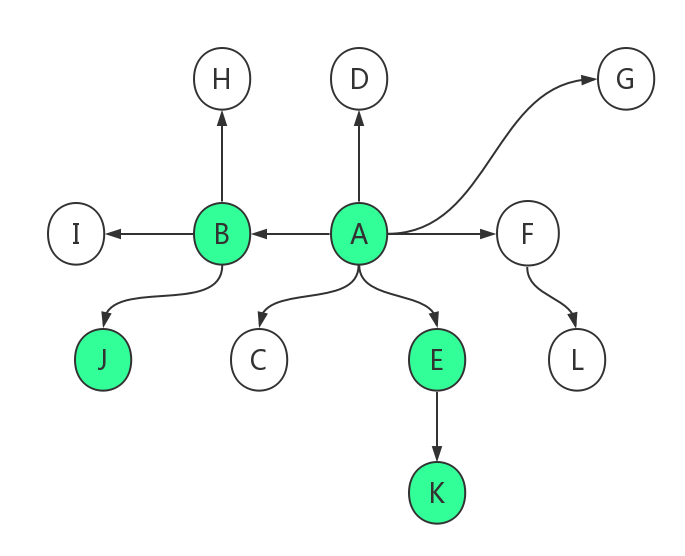
\includegraphics[width=0.5\textwidth]{USER}
    \bicaption{消息在用户网络上的传播过程}{The spread of news on the user's network}
    \label{fig:user}
\end{figure}

\item 地域特征反映了 Hashtag 存在明显的地理因素,不同地域的人关注的焦 点不同,因此具有明显的地域分布,结果展示如表\ref{tab:3_6_localtion}所示,某些主题标签带有明显的地域色彩,因此利用地域特征进行分组,形成 Hashtag 的局部聚类,有效 地表达了不同聚类结果。通过加入地域特征,可以将数据有效分组, 当去掉地域 特征以后,模型的性能下降很多,MAE 提高了 15.8\%,MSLE 提高了 16\%。
\begin{table}[H]
\newcommand{\tabincell}[2]{\begin{tabular}{@{}#1@{}}#2\end{tabular}}
    \centering
    \footnotesize% fontsize
    \bicaption{主题标签的地域特征}{Geographical characteristics of topic labels}
      \label{tab:3_6_localtion}
    \setlength{\tabcolsep}{8pt}% column separation
    \renewcommand{\arraystretch}{1.2}%row space 
    \begin{tabular}{c|c|c}
        \hline
       \textbf{ 地区} & \textbf{具体地区}& \textbf{Hashtag } \\
        %\cline{2-9}% partial hline from column i to column j
        \hline
		\textbf{海外} &中国以外的其他国家& \tabincell{c}{韩国水晶防晒喷雾,\\龟岛,龟梨和也} \\ \hline
		\textbf{东三省}&黑龙江, 吉林, 辽宁 & \tabincell{c}{二人转, 雾凇岛,\\冰雪大世界} \\ \hline
		\textbf{西北}& 青海, 新疆, 宁夏, 甘肃, 陕西& \tabincell{c}{羊肉泡馍, 青海湖旅游攻略\\西北贫困地区的孩子们一起成长} \\
        	\hline
    \end{tabular}
     
\end{table}


\item 主题特征对于 Hashtag 的预测十分重要, 当去掉主题特征时,模型的性能 下降很多,MAE 提高了 20\%,MSLE 提高了 18\%,反映出主题特征对于流行度 预测的重要性。不同 Hashtag 的主题特征如表3.11所示,从表中可知虽然是同一 个 Hashtag,但是随着时间的变化,其主题特征也会发生相应的变化,抽取不同 时刻的主题词来表示不同时刻的用户关注的焦点,对于主题标签的流行度预测 是具有重要参考价值的,因此刻画其主题特征是十分有必要的。

\begin{table}[H]
\newcommand{\tabincell}[2]{\begin{tabular}{@{}#1@{}}#2\end{tabular}}
    \centering
    \footnotesize% fontsize
    \bicaption{主题特征随着时间的变化
}{Topic features change over time}
      \label{tab:3_6_topic}
    \setlength{\tabcolsep}{6pt}% column separation
    \renewcommand{\arraystretch}{1.2}%row space 
    \begin{tabular}{c|c|c|c}
        \hline
       \textbf{ Hashtag} & \textbf{day-1 }& \textbf{day-2 }& \textbf{day-3}  \\
        %\cline{2-9}% partial hline from column i to column j
        \hline
		\textbf{文化新闻脱又秀} & \tabincell{c}{优酷, 分享, 新闻,
		\\故事, 沙和, 文化,
		\\微笑, 老师, 客户,
		\\一起, 看看} &  \tabincell{c}{今波, 贞观, 李世民,
		\\孟姜女哭, 土豆, 文化,
		\\天子, 新闻, 故事,
		\\什么, 中国, 下载} & \tabincell{c}{今波, 季-, 朱由校,
		\\秘招, 文化, 新闻,
		\\故事, 花絮, 独家,
		\\明朝, 皇帝, 救国,
		\\个人, 前世, 八仙,
		\\ 今生, 录制, 爱好, 中国}\\ \hline
		
		\textbf{周杰伦中国好声音} & \tabincell{c}{冯小刚, 声音, 大赞,
		\\领悟力, 宣传片, 给力,
		\\奥特曼, 才情, 满分,
		\\电影, 幽默, 合作} & \tabincell{c}{声音, 杰伦, 我的,
		\\偶像, 中国, 一直,
		\\我家, 歌词, 只有,
		\\随便, 超级, 长大,
		\\ 忘记, 出来, 好听} & \tabincell{c}{叶湘伦, 忽高,
		\\颜值, 只服, 周杰伦歌迷,
		\\后援会, 声音, 音乐,
		\\杰伦, 拜拜, 窒息,
		\\ 崩溃, 中国, 现场,
		\\赶往, 录制} \\ \hline
		
		\textbf{家族世代} & \tabincell{c}{信托, 视野, 观点,
		\\商界, 全球, 中外,
		\\大佬, 产品, 18 年,
		\\人物, 所有, 结果,
		\\默默无闻, 帝国} & \tabincell{c}{行善, 莫忘, 订阅,
		\\ 微信, 简史, 任正非,
		\\信托, 工具, 观点,
		\\斗争, 对方, 制度,
		\\迷茫, 政经, 技术} & \tabincell{c}{美国通用, 海尔, 惊天,
		\\马云, 王健林, 订阅,
		\\ 微信, 5 年, 56 亿美金,
		\\ 沉寂, 筹谋, 背后,
		\\故事, 年前, 人物} \\ 
        	\hline
    \end{tabular}
     
\end{table}

\end{enumerate}

在全部的特征集合上,本文衡量了全部特征重要性的集合,选取前 30 维最 重要的特征,如表\ref{tab:3_9}所示。通过对特征重要性的排序,本文发现时间序列是最 重要的,并且在整个时间序列特征中,开始时刻的时间序列特征是最重要的,反 映了开始时刻的长期影响,这个是本文的一个发现,并且通过选取前 30 维特征, 在可以牺牲一些精度的前提下,可以大幅度提高运算速度,对于后续优化提供了 思路。同时时间序列特征的效果最好,对整个预测任务最有用,这个是最重要的 特征,充分说明 Hashtag 存在明显的时间序列分布,对于后续 Hashtag 流行度的 预测提供了参考。另一方面,通过特征重要性的分析,可以看出本文针对主题标 签流行度预测提出的用户粉丝网络结构特征,主题特征,以及地域特征具有较高 的重要性,充分说明了该特征的有效性。



\begin{table}[H]
    \centering
    \footnotesize% fontsize
         \bicaption{ xgboost 特征重要性排序前三十维}{Xgboost feature importance prioritization of thirty dimensions}
      \label{tab:3_9}
    \setlength{\tabcolsep}{15pt}% column separation
    \renewcommand{\arraystretch}{1.2}%row space 
    \begin{tabular}{cccc}
        \hline
        \textbf{Rank} &  \textbf{Feature} &\textbf{ Rank} & \textbf{Feature}  \\
        %\cline{2-9}% partial hline from column i to column j
        \hline

       1 & 时间序列特征 & 16 & 主题向量-第十二维 \\
       2 &省地域特征-第十维& 17& 主题向量-第十五维 \\
       3 &地区地域特征-第一维 & 18 &地区地域特征-第七维\\
      4 & 微博长度 &19 &  用户向量-第十维\\
       5 & 主题向量-第一维 &20 &    地区地域特征-第二维\\
       6 & 消息类型 &21 & 朋友数   \\
       7 & 主题向量-第五维 &22& 微博情感性\\
        8&      是否包含 URL &23 &   省地域特征-第三维 \\
             9&评论数 &24 & 地区地域特征-第六维  \\
       10 &       转发数 & 25 & 用户向量-第三十四维  \\
             11 &省地域特征-第二十维 &26 & 主题向量-第十九维 \\
       12 &       主题向量-第十维 &27 & 省地域特征-第九维 \\
       13&地区地域特征-第五维 &28 & 是否包含数字    \\
          14 &用户向量-第四维 &29 & 用户向量-第五十二维  \\
            15 & 粉丝数 &30 & 用户向量-第六十四维    \\



      
      
        	\hline
    \end{tabular}

\end{table}


\section{本章总结}
传统的主题标签流行度预测方法主要是基于时间序列特征,内容特征,很少 考虑主题标签的自身特性以及考虑消息在用户粉丝网络结构上的传播机制,因 此提出了一种基于多维度特征的主题标签流行度预测算法,基于用户粉丝网络 结构特征,刻画消息在用户之间的传播特性,时间序列特征,主题特征,地域特 征,Hashtag 自身特性以及用户特征等多系列不同维度的特征,结合 xgboost 机器 学习模型,得到了较好的流行度预测效果。同时本文对于提出的 Hashtag 自身特 性,地域信息以及用户粉丝网络结构特征的重要性进行了分析,实验结果表明添 加这几类新的特征以后,模型效果有了较大的提升,验证了这几类特征在主题标 签流行度预测上的重要性,对于后续主题标签流行度预测提供了新的研究方向。


\chapter{基于多源头的主题标签流行度预测}\label{chap:four}

在第三章中,我们介绍了宏观角度的 Hashtag 流行度预测方法,主要是使用 机器学习的方法,人工构造有效特征来进行预测,该方法的好坏很大程度上取决 于人工构造的特征的质量。通过对大多数的 Hashtag 流行度预测案例来看,基于 特征的 Hashtag 流行度预测需要一下几个条件:足够的观测时间窗又,通过大量 观测时间窗又内的数据获取有效的宏观特征;另外需要 Hashtag 本身具有足够的 传播规模。而这些约束条件在某些预测场景下并不满足,而微观视角是从理解传 播过程入手,建模参与用户与传播环境的反馈以及对最终流行度的影响,因此更 适宜解决宏观视角所不能解决的情况。另外基于生成式的消息建模方法不是预 测未来的流行度,因此预测性能是有缺失的。另外消息流行度预测问题解决的是 单源头问题,因此对于多源的 Hashtag 流行度预测建模是目前的研究方向。

针对以上问题,本章提出了一种建模多源 Hashtag 流行度预测的模型,该模 型既可以有效学习每个源头内部的传播方式,又可以通过 attention 机制考虑不 同源头之间的影响,从而刻画整体模型的传播机制。然后使用 TensorFlow 平台 进行了模型训练和测试,通过实验证明了模型的有效性。
\section{问题描述和基本思路}
\subsection{问题描述和基本思路}
目前社交网络中的消息流行度预测都是单源头的问题,每条消息只有一个 源头。此类模型主要是建模从该单一消息源头转发的路径关系。然而,目前常 见的消息流行度预测方法无法很好的建模 Hashtag 流行度预测问题。因为对于同 一个 Hashtag,它可以在不同时刻由不同的用户发出,它的源头不是唯一的,如 何很好的刻画多源头之间的关系是十分必要的。因为对于同一个 Hashtag,当微 博上的一个大 V 用户发出,它的转发量很可能是暴涨的,而对于一个普通用户 发出的,它的转发量可能是很稀少的, 如图4.1所示,重要节点的转发关系是庞大 的,因此刻画每个源头的重要性是十分必要的。另一方面,还需考虑每个源头之 间的传播方式,单独建模好每一个源头的数据对于整体的效果也是十分重要的。 综合考虑这两种方式的优缺点,本章提出了一种既建模了单个源头序列之间的 传播关系又考虑了多个源头之间关系的模型。

为了更好的刻画 Hashtag 传播过程中的机制,本章进行小时级别的数据划分,当一个 Hashtag 由一个源头发出以后 1 小时,分析该 Hashtag 未来 24 小时内 的转发数量。

\begin{figure}[H]
    \centering
    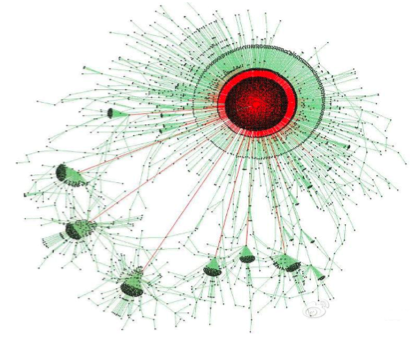
\includegraphics[width=0.5\textwidth]{hashtag_19}
    \bicaption{消息传播方式}{Message dissemination}
    \label{fig:4_2}
\end{figure}

\subsection{基本思路}


目前现有的 Hashtag 流行度预测基本都是基于特征的方法,没有建模它们内 部的传播机制,同时微博消息的流行度预测算法虽然很好的建模了消息的内部 传播机制,但是无法很好的适用到多源头 Hashtag 的流行度预测问题上。为了建 模多源头 Hashtag 流行度预测问题,可以借助算法中的分而治之的思想,既要很 好的建模每一个源头上的消息传播机制,又很好的将每个源头的数据融合在一 起,从而在整体上刻画 Hashtag 的流行度预测模型。

因此,本章的基本思路是首先根据消息传播机制的方式建模 Hashtag 每一个 源头中消息的转发情况,然后对于每一个源头的传播路径得到一个高维表达,通 过 attention 机制衡量每一个源头的重要性,来建模整体的 Hashtag 流行度预测过 程。

\section{相关工作}
由于本文的主要建模办法是采用 attention 机制来刻画 Hashtag 不同源头之间 的重要性,所以首先介绍一下 attention 的基本原理,然后介绍一种刻画消息内部 传播机制的模型,便于后续模型的提出。
\subsection{attention 机制}

Attention 模型最初主要是应用于图像识别中,它主要是模仿当人观看一副 图像时,视线的焦点在物体上的移动。当模型对图像或语言进行识别时,每次集 中于部分重要特征上,识别更加准确。现在在很多自然语言处理的任务上应用也 很多,比如文本分类中,用 attention 来衡量不同词的重要性。然而如何衡量特征 的重要性呢,最直观的方法就是考虑每个特征的权重,因此,Attention 模型的结 果就是在每次识别时,首先计算每个特征的权重,然后对特征进行加权求和,权 值越大,该特征对当前模型的贡献就越大,自动选取到了重要的特征。

机器翻译中的 Attention 模型最直观\citep{Luong2015Effective},并且易于理解,每当生成一个单 词时,找到源句子中与其对应的单词,翻译才准确。此处就以机器翻译为例来讲 解 Attention 模型的基本原理,在介绍 Attention 模型之前,需要先介绍一下机器 翻译领域应用最广泛的模型——Encoder-Decoder(编码-解码)结构 \citep{Bahdanau2014Neural}。

Encoder-Decoder 框架包括两个步骤,第一步是 Encoder(编码),将输入数据 (如图像或文本)编码为一系列特征,第二步是 Decoder(解码),以编码的特征作 为输入,将其解码为目标输出。Encoder 和 Decoder 是两个独立的模型,可以采 用神经网络,也可以采用其他模型进行训练。机器翻译中的 Encoder-Decoder 示
例如图\ref{fig:4_3}所示。该示例将一个句子(ABC)翻译为另一种语言的句子(WXYZ), 其中 A、B、C 和 W、X、Y、Z 分别表示一个字或一个单词,图中每个方框表示 一个循环神经网络模型,不同的方框表示不同时刻的表达,<EOS> 表示句子的 结束。


\begin{figure}[H]
    \centering
    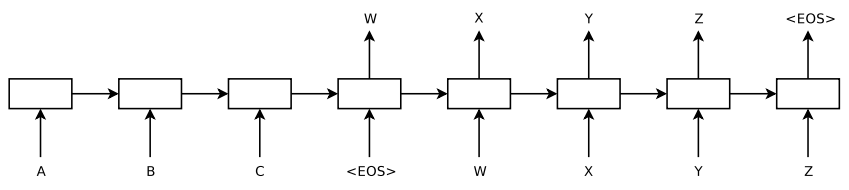
\includegraphics[width=0.5\textwidth]{hashtag_20}
    \bicaption{编码-解码}{Encoder-Decoder}
    \label{fig:4_3}
\end{figure}


Attention 机制在 Encoder-Decoder 中介于 Encoder 和 Decoder 中间,首先根 据 Encoder 的特征计算权值,然后对 Encoder 的特征进行加权求和,作为 Decoder 的输入,其作用是将 Encoder 的特征以更好的方式呈献给 Decoder,找到每个词 对应的重要输入,更好的反映编码与解码之间的关系, 模型如图\ref{fig:4_4}所示,图中的 $a_{t,i}$,i 就是 Attention 模型生成的权值。

\begin{figure}[H]
    \centering
    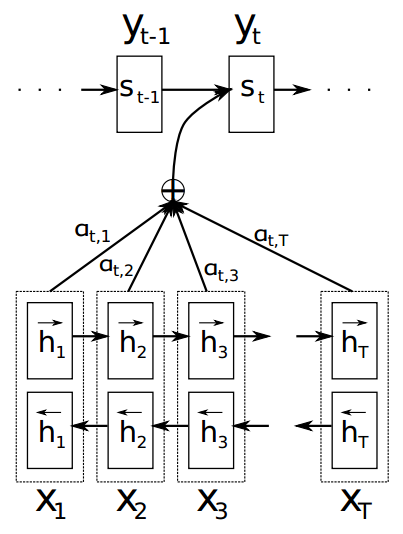
\includegraphics[width=0.5\textwidth]{hashtag_21}
    \bicaption{基于注意力的编码解码过程\citep{Bahdanau2014Neural}}{Attention-based encoder and decoder process\citep{Bahdanau2014Neural}}
    \label{fig:4_4}
\end{figure}

在 t 时刻,对特征 $h $进行加权组合,那么生成新的单词的过程如公式\ref{eq:4_1}所 示, 这里的 $f\_{att}$ 才是 Attention 模型的核心,可以用来估计位置 i 附近的输入和位 置 t 的输出之间的匹配程度,它的表达是不唯一的,常见的是使用一个神经网络 来进行拟合。

\begin{equation}\label{eq:4_1}
	\begin{cases}
	c_t = \sum_{i=1}^T a_{t,i}h_i \\
	a_{t,i} = \frac{\exp(e_{t,i})}{\sum_{k=1}^T \exp(e_t,k)} \\
	e_{t,i} = f_{att}(s_{t-1},h_i)\\
	f_{att}(s_{t-1},h_i) = \tanh(W_as_{t-1} + U_ah_i)
	\end{cases}
\end{equation}

\subsection{DeepHawkes 模型}


在第二章的相关工作中,本文已经详细介绍过了 DeepHawkes 模型 \citep{Cao2017DeepHawkes},它 使用神经网络进行消息流行度预测,该模型既可以建模消息的内部传播机制,又 将消息的未来流行度作为目标进行预测,是目前不错的消息流行度预测模型。但 是在其建模消息传播机制中的时间衰减影响的时候,该模型学习到的是一个固 定结果, 如图\ref{fig:4_5}所示,认为所有的数据在相同时刻的影响力是一样的。但是实际
 上相同时间段内的数据由于不同的传播路径,不同的路径长度等因素,导致它们 的影响力是不同的,因此本文对其进行改进,使用 attention 来刻画每个过程的影 响,既考虑时间衰减的影响又加上传播路径的信息,更加全面的刻画不同路径的 权重。
\begin{figure}[H]
    \centering
    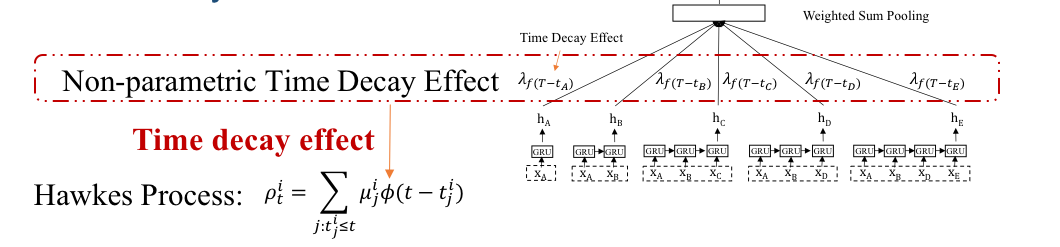
\includegraphics[width=1\textwidth]{hashtag_22}
    \bicaption{DeepHawkes 模型中的时间衰减影响\citep{Cao2017DeepHawkes}}{Time Decay Effect in DeepHawkes Model\citep{Cao2017DeepHawkes}}
    \label{fig:4_5}
\end{figure}

\section{多源 Hashtag 流行度预测模型}
考虑到消息传播中的单源传播模型无法很好的刻画多源 Hashtag 流行度预
测问题,结合 attention 机制,本章提出了一种多源 Hashtag 流行度预测模型。
\subsection{模型结构}

本章提出了一种基于 attention 的多源头 Hashtag 流行度预测模型。模型的结 构如图\ref{fig:4_6}所示, 主要由以下几部分组成:

\begin{enumerate}
\item 首先通过 LINE,将用户网络粉丝结构生成每个用户的向量表达,作为传 播路径上的每个用户的输入;
\item 然后将Hashtag传播路径进行编码,通过循环神经网络进行建模,刻画每 个源头上 Hashtag 的传播机制;
\item 通过考虑序列间的 attention 机制,刻画相同源头上 Hashtag 不同传播路 径的影响力;
\item 通过考虑不同源头的 attention 机制,刻画每一个 Hashtag 源头对于整体 Hashtag 流行度的影响;
\item 最后通过神经网络全连接来预测目标值。

\end{enumerate}

\begin{figure}[H]
    \centering
    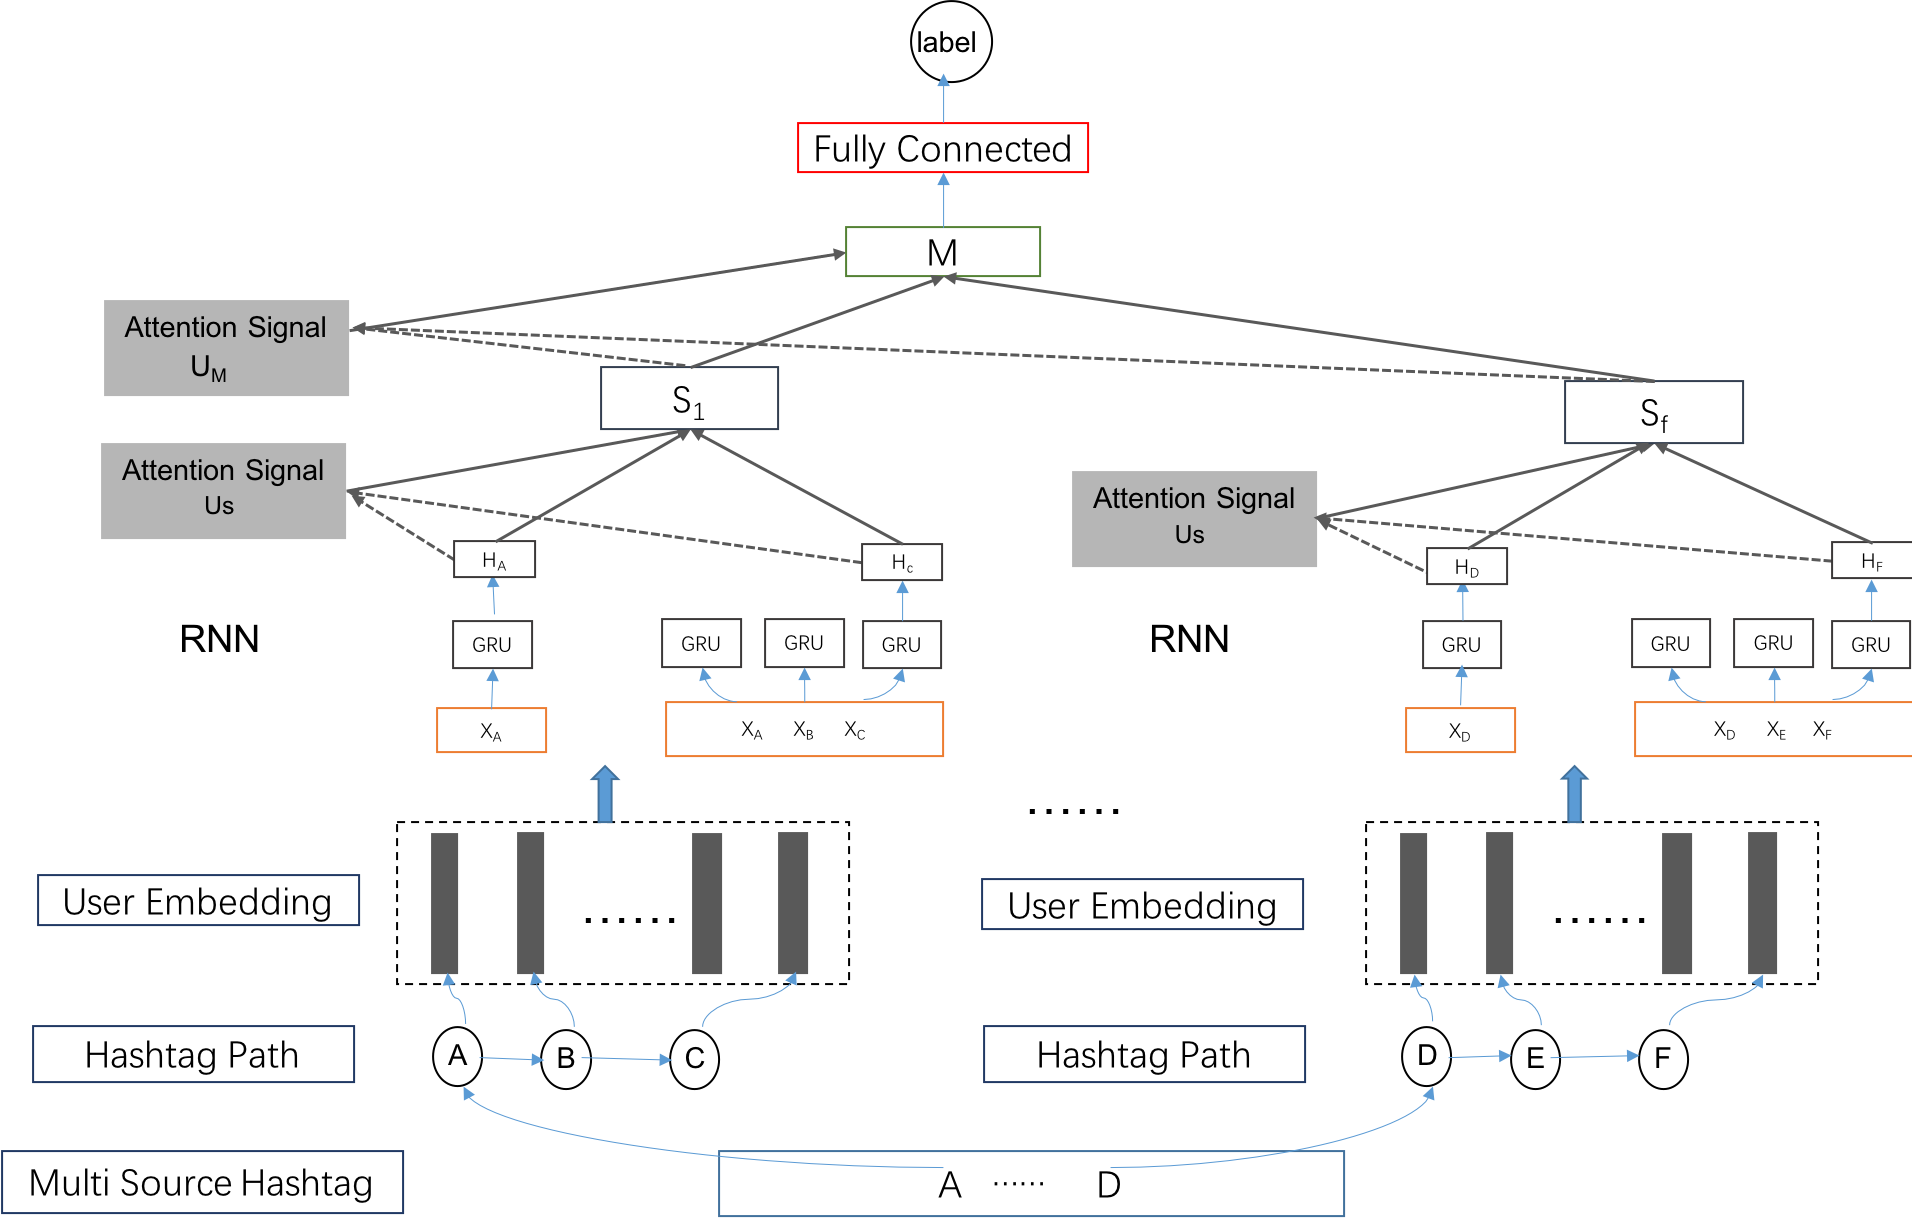
\includegraphics[width=1\textwidth]{model}
    \bicaption{基于注意力的多源 Hashtag 流行度预测}{Multi-source Hashtag popularity prediction based on attention}
    \label{fig:4_6}
\end{figure}

与传统的 Hashtag 流行度预测模型相比,本章提出的模型有如下几个创新 点:
\begin{enumerate}
\item 之前的 Hashtag 流行度预测都是基于特征的方式,本文第一次采用神经 网络建模主题标签的传播方式,便于理解影响 Hashtag 流行度的因素;
\item 对于传统的消息时间衰减影响,本文采用 attention 机制进行学习,有效 刻画每个元素的影响;
\item 本文对于多源头的 Hashtag 进行建模,通过 attention 机制刻画不同源头 的重要性。

\end{enumerate}

\subsection{User Embedding Layer}
User Embedding Layer 把每一个用户映射成一个分布式向量表示,user embedding 有两个好处,第一个是可以自动学习用户的分布式表示,第二个好处是 可以大大缩小参数空间,加快训练速度。在这里,本文使用了预训练的方式,首 先,使用 LINE 模型根据用户粉丝网络结构进行用户分布式学习,得到网络结构 中每个用户的分布式表示,作为模型里面出现的用户的初始化表示,这样通过 加入先验知识的方式可以提高模型的训练速度,同时减少过拟合,将用户向量 刻画的更细致;并且根据第三章的内容可以得知用户的粉丝网络结构特征对于Hashtag 流行度预测是有一定作用的,因此可以提高模型的效果。

\subsection{RNN Layer}

对于 Hashtag 多源头中的每一个源头消息,较好的刻画其具体传播特性对于 整体的预测效果是十分重要的。在转发过程中,每一次的转发都可能改变未来转 发的情况,在实际情况中,不仅当前转发用户本身对于未来转发有影响,而整个 转发路径也会有所贡献。因此,本层不仅仅对当前转发用户进行建模,而是通过 递归神经网络对整个转发路径进行编码。这种做法主要是出于两点考虑:一个 是影响的传递性,以前的参与者不仅影响其直接转发者,而且通过转发方式对 间接转发者产生影响,因此整个转发路径上的每个用户都会对后续转发产生影 响;另一个是结构位置信息,通过用户在转发路径上出现的次数来表征,来衡量 用户的重要性,如图\ref{fig:cascade}所示, 节点 B 在整个消息传播过程中是十分重要的,总之 该层主要是对整个转发路径进行建模。通过以上分析,因此本层使用 GRU,一 种 RNN 的变形体进行序列建模,对于每个序列输入 [$X_{A},X_{B},X_{C}...X_{N}$], 通过 GRU 得到得到每一序列的输出$H_{A}$, 公式如\ref{eq:4_1_g}所示。由于每个序列的长度是不固定的, 因此对于每个序列的输出,本文选取最后一个实际的节点作为循环神经的输出, 这样考虑了数据的有效性。

\begin{equation}\label{eq:4_1_g}
H_A = GRU([X_A,X_B,X_C...X_N])
\end{equation}

\begin{figure}[H]
    \centering
    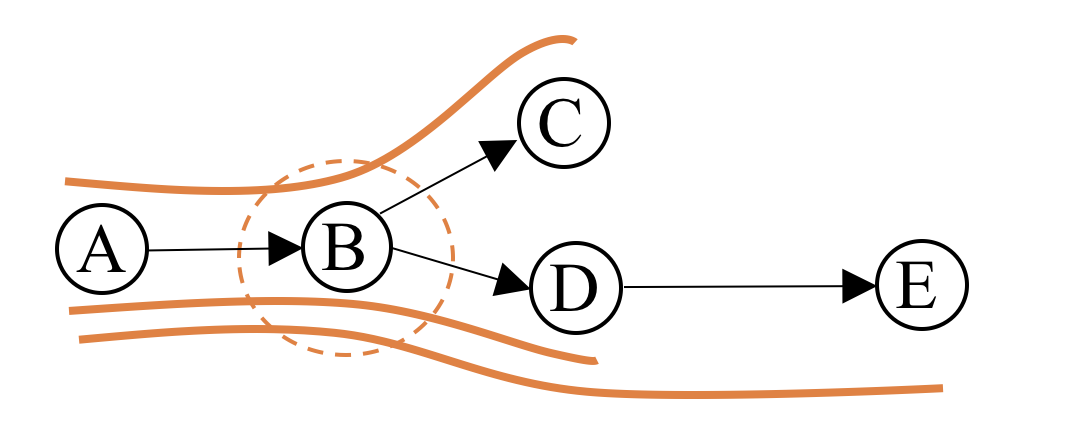
\includegraphics[width=0.8\textwidth]{cascade}
    \bicaption{消息级联传播展示图}{Message cascade display}
    \label{fig:cascade}
\end{figure}

\subsection{第一层 attention}
已有的研究证明了时间衰减对消息传播的影响,但是传统的方式都是需要 建模时间衰减函数,然而在不同的领域,这个函数很可能是不一样,因此很难建 模。为了避免以上问题,因此本文采用 attention 机制,考虑每个序列的 GRU 输出以及此时刻的时间因素,自动学习每个序列的时间衰减影响,最终的结果输出 $S_{i}$如公式\ref{eq:4_1_a}所示。公式里面的$H_{it}$表示上一层的序列输出,$T_{it}$表示该序列的时 间间隔因素,$U_{S}$ 表示 attention 的上下文向量,是一个高维向量表示,这个向量 通过随机初始化得到,并不断学习,$S_{i}$ 表示 attention 层的输出。

\begin{equation}\label{eq:4_1_a}
	\begin{cases}
	u_{it} = \tanh(W_S(H_{it}+T_{it}) +b_S)\\
	\alpha_{it} = \frac{\exp(u_{it}U_S)}{\sum_{t} \exp(u_{it}U_S)} \\
	S_i = \sum_{t}\alpha_{it} H_{it}
	\end{cases}
\end{equation}

\subsection{第二层 attention}

对于多源头的 Hashtag 流行度预测,由于每个源头的重要性是不同的,如何 衡量它们之间的重要性和区分度是本研究的难题。为了更好的刻画每个源头的 重要性,本文采用 attention 机制,对于每一个源头计算一个权重,然后求得最终 的结果,公式如\ref{eq:4_2_a}所示,公式中的 $S_{i}$ 表示每个源头的向量表达,$U_{M}$是一个源 头级别的上下文向量, 该向量通过随机初始化然后不断学习,向量 M 表示最后的 多源头向量的整合。

\begin{equation}\label{eq:4_2_a}
	\begin{cases}
	u_i = \tanh(W_mS_i +b_m)\\
	a_i = \frac{\exp(u_iU_M)}{\sum_{i} \exp(u_iU_M)} \\
	M = \sum_{i}\alpha_i S_i
	\end{cases}
\end{equation}

\subsection{全连接层}
模型的最后一层是多层感知机,通过将上一层 attention 的输出 M 作为本层
 的输入,本层的输出直接是最终的目标,公式如\ref{eq:m_1}所示:

\begin{equation}\label{eq:m_1}
Label = MLP(M)
\end{equation}
模型的最小化的目标函数如\ref{eq:o_1}所示:


\begin{equation}\label{eq:o_1}
obj = \frac{1}{N}\sum_{i=1}^N(\log Prediction - \log Label)^2
\end{equation}

公式里面的N表示全部的Hashtag的数量,prediction代表预测值,label表示真实值,通过取对数的方式可以降低离群点的影响,模型更加便于优化。

\subsection{模型实现}


本文的模型是使用 Tensorflow 平台实现的 \citep{Abadi2016TensorFlow},如图所示\ref{fig:4_1},TensorFlow 是 一个采用数据流图(data flow graphs),用于数值计算的开源软件库。节点(Nodes) 在图中表示数学操作,图中的线(edges)则表示在节点间相互联系的多维数据 数组,即张量(tensor)。它灵活的架构让你可以在多种平台上展开计算,例如台 式计算机中的一个或多个 CPU(或 GPU),服务器,移动设备等等。TensorFlow 最初由 Google 大脑小组(隶属于 Google 机器智能研究机构)的研究员和工程师 们开发出来,用于机器学习和深度神经网络方面的研究,但这个系统的通用性使 其也可广泛用于其他计算领域。

\begin{figure}[H]
    \centering
    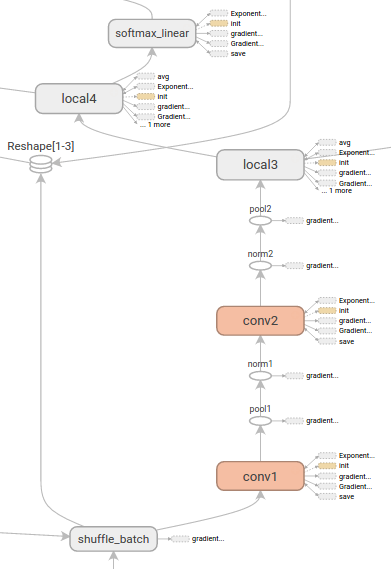
\includegraphics[width=0.5\textwidth]{hashtag_18}
    \bicaption{Tensorflow数据流动示意图}{Tensorflow data flow diagram}
    \label{fig:4_1}
\end{figure}

本文使用的是 Tensorflow1.6 ,根据官网的版本说明,Tensorflow 具有如下特 点:
\begin{enumerate}

\item \bfseries 性能最优化\mdseries 

由于 Tensorflow 给予了线程、队列、异步操作等以最佳的支持,Tensorflow 让你可以将你手边硬件的计算潜能全部发挥出来。你可以自由地将 Tensorflow图中的计算元素分配到不同设备上,Tensorflow 可以帮你管理好这些不同副本。

\item  \bfseries 灵活使用 \mdseries  

TensorFlow 不是一个严格的“神经网络”库。只要你可以将你的计算表示为 一个数据流图,你就可以使用 Tensorflow 来构建图,描写驱动计算的内部循环。 Tensorflow 提供了有用的工具来帮助你组装“子图”(常用于神经网络),当然用户 也可以自己在 Tensorflow 基础上写自己的“上层库”。定义顺手好用的新复合操作 和写一个 python 函数一样容易,而且也不用担心性能损耗。当然万一你发现找 不到想要的底层数据操作,你也可以自己写一点 c++ 代码来丰富底层的操作。

\item   \bfseries 高效开发\mdseries 

TensorFlow 保证了 Python API 稳定性,可以在不破坏现有的代码基础上获 取新功能。

\end{enumerate}

综上所述,Tensorflow 的出现大大方便了深度学习研究者们快速实现部署自 己的模型,用于机器学习和深度神经网络方面的研究。本章的模型部署在 Ten- sorflow 上,使用 GPU 加速训练,在模型训练阶段,使用随机梯度下降算法,在 整个实验过程中,本文观察到大概训练时间只需 3 个小时左右,模型就在训练数 据上收敛了。


\section{实验结果及分析}

\subsection{实验数据}
本章从微观角度刻画 Hashtag 流行度预测,将 Hashtag 的观测范围限定到一 小时内,然后预测二十四小时后的流行度。对于用到的用户粉丝网络结构数据依 然采取第三章的数据,其他数据如下。

用于提取 Hashtag 的数据如下,一共四百三十万左右的 Hashtag 数据,从这 些数据中构建训练样本。
\begin{table}[H]
    \centering
    \footnotesize% fontsize
         \bicaption{多源头 Hashtag 数据}{Multi-source Hashtag data}
      \label{tab:multi_h}
    \setlength{\tabcolsep}{30pt}% column separation
    \renewcommand{\arraystretch}{1.2}%row space 
    \begin{tabular}{cccc}
        \hline
       编号& 属性& 属性值 \\
        1 & 文件大小 & 1.1G\\
        2 & Hashtag 的消息数量 & 4322622\\
        %\cline{2-9}% partial hline from column i to column j
        \hline
        
        	\hline
    \end{tabular}

\end{table}
从以上数据构建多源头 Hashtag 训练样本,样本总数一共六万三千左右,训 练样本和验证样本大概七比一。

\begin{table}[H]
    \centering
    \footnotesize% fontsize
         \bicaption{多源头 Hashtag 训练样本数据}{Multi-source Hashtag training sample data}
      \label{tab:sample_hashtag}
    \setlength{\tabcolsep}{30pt}% column separation
    \renewcommand{\arraystretch}{1.2}%row space 
    \begin{tabular}{cccc}
        \hline
        编号 & 属性 & 属性值\\
        1 & 文件大小& 150M\\
        2 &Hashtag 训练样本数目& 63487\\
        %\cline{2-9}% partial hline from column i to column j
        \hline
        
        	\hline
    \end{tabular}

\end{table}

\subsection{评价指标}
模型在训练数据上进行训练,然后在测试数据上进行验证。针对测试数据中
的每一个 Hashtag, 本文预测其未来的流行度,采用如下评价指标进行评估:

 MSLE(mean squared log error)公式如\ref{eq:msle}所示, 函数计算了一个对应平方对数 (二次)误差或损失的预估值风险度量, 由于 Hashtag 的分布呈现幂率分布,因此
通过 log 运算,该指标更加适合具有指数增长趋势的数据。 

 \begin{equation}\label{eq:msle}
 	MSLE = \frac{1}{N}~\sum_{t=1}^N~(\log{(observed_t + 1)} - \log{(predicted_t + 1)})^2
 \end{equation}
 
 mSLE(median squared log error)公式如\ref{eq:mmsle}所示,该函数有趣有趣,因为它的离群值很强. 通过取目标和预测之间的所有 sle 的中值来计算损失.
 
  \begin{equation}\label{eq:mmsle}
  	\begin{split}
       mSLE = median((\log{(observed_1 + 1)} - \log{(predicted_1 + 1)})^2,...,\\
      ( \log{(observed_N + 1)} - \log{(predicted_N + 1)})^2)
       \end{split}
  \end{equation}

\subsection{结果分析}
\subsubsection{参数设置}
深度学习模型的特点之一就是有很多参数需要调整,本模型也不例外,参 数主要分为两类,一类是模型参数,一类是训练参数。模型参数比如每一层的特 征维度,attention 的大小,user embedding 的大小等等;训练参数,比如学习率, batch 大小,dropout 等等,这些参数对于模型结果都会产生很大影响。

论文主要采用网格搜索方法寻找最优参数,既先固定其他参数,然后调整某 个参数到最优,依次类推,找到每一个参数的最优,模型所用到的主要参数,含 义以及最终值如表\ref{tab:model_1}所示。

\begin{table}[H]
    \centering
    \footnotesize% fontsize
     \bicaption{模型参数表}{Model parameter table}
      \label{tab:model_1}
    \setlength{\tabcolsep}{30pt}% column separation
    \renewcommand{\arraystretch}{1.2}%row space 
    \begin{tabular}{cccc}
        \hline
        \textbf{模型参数}&\textbf{ 含义}&\textbf{ 取值} \\
        %\cline{2-9}% partial hline from column i to column j
        \hline
        \textbf{user~embedding} & 用户向量维度&  100\\
       \textbf{ sequences} &序列长度 &1000 \\
     \textbf{   steps }& 序列个数& 30\\
       \textbf{ $U_{S}$ }&局部序列 attention 上下文向量 & stddev=0.01\\
       \textbf{ $U_{M}$}&全局 attention 上下文向量 & stddev=0.01 \\
\textbf{        Fully Connected Layer} & 全连接的初始值&  [-1,1]\\
        	\hline
    \end{tabular}
    
\end{table}


模型训练所用到的主要参数,含义以及最终值如表\ref{tab:model_2}所示。

\begin{table}[H]
    \centering
    \footnotesize% fontsize
         \bicaption{模型训练参数}{Model training parameters}
      \label{tab:model_2}
    \setlength{\tabcolsep}{30pt}% column separation
    \renewcommand{\arraystretch}{1.2}%row space 
    \begin{tabular}{ccc}
        \hline
       \textbf{ 训练参数} & \textbf{含义} & \textbf{取值}   \\
        %\cline{2-9}% partial hline from column i to column j
        \hline
        \textbf{alpha }& 学习率 & 0.005 \\
        \textbf{rate~ for~ embedding} &用户 embedding 的学习速率&0.0005 \\
       \textbf{ dropout} & 正则大小 &0.8 \\
        \textbf{batch ~size} & 每批的大小& 32 \\
      \textbf{  l2 }& 正则项大小
  &0.05\\
        	\hline
    \end{tabular}

\end{table}

在这里,本文发现参数的设置对模型效果影响比较大,合适的参数加上合理 的模型结构,加上正确的优化目标才能够使模型达到最优效果,这三者缺一不 可。

\subsubsection{模型间对比}
为了验证模型的有效性,本文所采用的对比模型主要包括如下几种:
\begin{enumerate}
\item Model1 首先通过 DeepHawkes 模型对 Hashtag 的每个源头的数据进行分 别预测,然后将预测的结果求和,这个是最基础直观的操作,作为基本的 baseline。
\item Model2 为了验证 attention 对于序列之间的权重的衡量,将 DeepHawkes 模型中的时间衰减影响换成 attention 机制,最后将预测的结果求和。
\item Model3 为了验证 attention 对于 Hashtag 不同源头之间的权重的衡量,将 DeepHawkes 模型每个源头的输出结合 attention 来作为整体的表达,然后进行整 体的预测。
\end{enumerate}


本文将基于多源头的 Hashtag 流行度预测模型,与以上三种模型进行试验对比,结果对比如表\ref{tab:model_r}所示。

\begin{table}[H]
    \centering
    \footnotesize% fontsize
         \bicaption{模型之间结果对比}{Comparison of results between models}
      \label{tab:model_r}
    \setlength{\tabcolsep}{30pt}% column separation
    \renewcommand{\arraystretch}{1.2}%row space 
    \begin{tabular}{ccc}
        \hline
        \textbf{Models }& \textbf{MSLE }&\textbf{ mSLE} \\
        %\cline{2-9}% partial hline from column i to column j
        \hline
	    \textbf{Model1} & 3.72 & 1.06\\
	    	    \textbf{Model2} & 3.64 & 1.02\\
	     \textbf{Model3} & 3.42 & 0.94\\
        \textbf{本模型} & 3.38 & 0.88\\
        	\hline
    \end{tabular}

\end{table}


根据实验结果,我们发现基于 attention 的多源头的 Hashtag 流行度预测模型 可以有效刻画 Hashtag 的传播机制,和单源头消息的流行度预测模型 DeepHakwes 相比,效果有了明显提升,MSLE 提升了 9\%,证明模型的有效性。并且通过 Model1 和 Model2 之间的对比,加入的序列间的 attention 确实对模型有一定的帮助,效 果提升不高,可能是因为时间衰减因素所占的比重较大,对整体的影响很重要。 另外通过源头的 attention,发现 model3 比 model1 的效果提升了很多,MSLE 提 升了 8\%, 验证了 attention 对于多源的有效刻画。

为了展示用户向量的初始化方式对于模型的整体效果以及计算性能的影响, 本文将通过用户向量随机初始化作为输入与通过 LINE 模型得到的用户向量表 示进行对比,结果展示如表\ref{tab:model_user}所示,通过实验可知,通过使用预训练的方式学 习到的用户向量表达,对于整体结果有一定的提升,因为通过模型学到的用户向 量表达,其实也是训练数据下的用户粉丝网络结构的缩影,学习到的一种局部表 达,通过使用 LINE 进行预训练得到用户的向量表达,更加全面的反映了用户之 间的关系,对于模型的预测提供了更加全面的参考,并且节约了用户向量学习的 时间,模型整体的计算时间大大减少, 时间效率提高了 30\% 左右,为以后模型的 优化以及性能的提升提供了参考方向。

\begin{table}[H]
    \centering
    \footnotesize% fontsize
         \bicaption{用户向量的初始化方式对比}{Comparison of user vector initialization methods}
      \label{tab:model_user}
    \setlength{\tabcolsep}{30pt}% column separation
    \renewcommand{\arraystretch}{1.2}%row space 
    \begin{tabular}{cccc}
        \hline
        \textbf{Models }& \textbf{MSLE }&\textbf{ mSLE} & \textbf{time}\\
        %\cline{2-9}% partial hline from column i to column j
        \hline
	    \textbf{本模型 + 随机初始化} & 3.44 & 0.95 & 13469s\\
        \textbf{本模型 +LINE} & 3.38 & 0.88 & 9546s\\
        	\hline
    \end{tabular}

\end{table}


\section{本章总结}

对于传统的基于特征的 Hashtag 流行度预测问题,需要人工构造复杂的特 征,并且无法建模 Hashtag 传播中的机制,无法理解其内部具体的传播过程;另 一方面基于神经网络的消息流行度预测问题虽然刻画了消息内部的传播机制, 但是它解决的是单源头问题,无法有效的处理多源头的 Hashtag, 并且内部的时 间衰减影响无法刻画每条传播途径的区别。因此本章提出了一种基于多源头的 Hashtag 流行度预测模型,通过深度学习自动学习特征,并且针对时间衰减效应 采用 attention 机制,来建模每条路径的影响,同时针对多源头 Hashtag 的传播, 采用 attention 建模每个源头的重要性,有效的将多个源头整合到一起,实现了多 源头的 Hashtag 流行度预测。之后,使用 Tensorflow 平台进行模型的训练,测试。 通过实验证明,与其他模型相比,本文提出的模型是有效的,与 DeepHawkes 模 型相比,MSLE 提升了 9.1\%。
\chapter{主题标签流行度预测模型的应用与部署}\label{chap:five}

本文第三章通过挖掘有效特征,实现了 Hashtag 宏观上的流行度预测模型, 本文第四章通过刻画 Hashtag 的传播机制,针对 Hashtag 多源性的特点,提出了 基于多源头的深度学习模型,是在这个问题上的首创。之后,为解决群体监测 中的事件热度预测,本文将基于特征的 Hashtag 流行度预测模型进行了应用与部 署,搭建了事件热度预测系统。

本章组织如下,首先介绍了事件热度预测系统的主要功能,然后介绍了该 系统的总体架构和预测流程,最后对于事件预测模块的设计细节和具体实现方 式进行详细阐述,包括微博数据模块,用户信息,事件预测模块以及日志记录模 块。

\section{事件热度预测系统}


事件热度预测系统是一个集各种舆情任务于一身的系统,目前有两个客户 端,一个是手机客户端,另一个是网页端,网页端的结果展示界面如图\ref{fig:figfivetwo}所示。 事件热度预测系统主要有如下几个功能:
\begin{enumerate}
\item 该系统可以自动采集微博,Twitter,Facebook 等消息。
\item 该系统能够根据用户需求,自定义任务关注的话题以及选择关注的时间 范围,并且还可以给用户推荐出目前的热点话题。
\item 该系统还可以根据用户任务,自动定时更新任务状态,对于事件热度可 以实时获取。
\item 对于预测结果,该系统抽取了部分微博消息进行展示,可以跳转到微博 的具体内容,使用户能够直观了解事件的具体内容。
\item 该系统可以通过对于历史数据的分析来进行线下预测,及时和用户的线 上预测数据进行对比。
\end{enumerate}

\begin{figure}[!htbp]
    \centering
    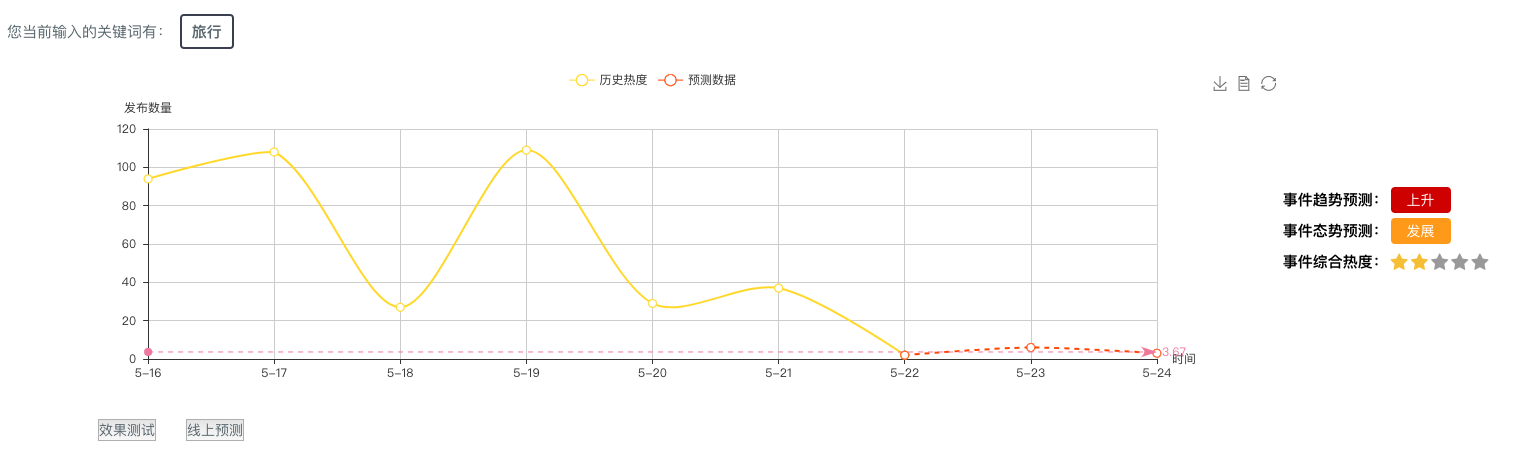
\includegraphics[width=1\textwidth]{fig_5_1_2_new}
    \bicaption{事件热度预测系统界面}{Public opinion data analysis system interface}
    \label{fig:figfivetwo}
\end{figure}

\section{系统架构}

事件热度预测系统架构如图\ref{fig:5_2}所示,本系统包含三个子系统,分别为业务 子系统,负责前端展示、任务提交、数据转发等功能,计算子系统负责核心算法 执行以及模型的更新,数据管理子系统负责和数据存储以及结果库的交互。

\begin{figure}[!htbp]
    \centering
    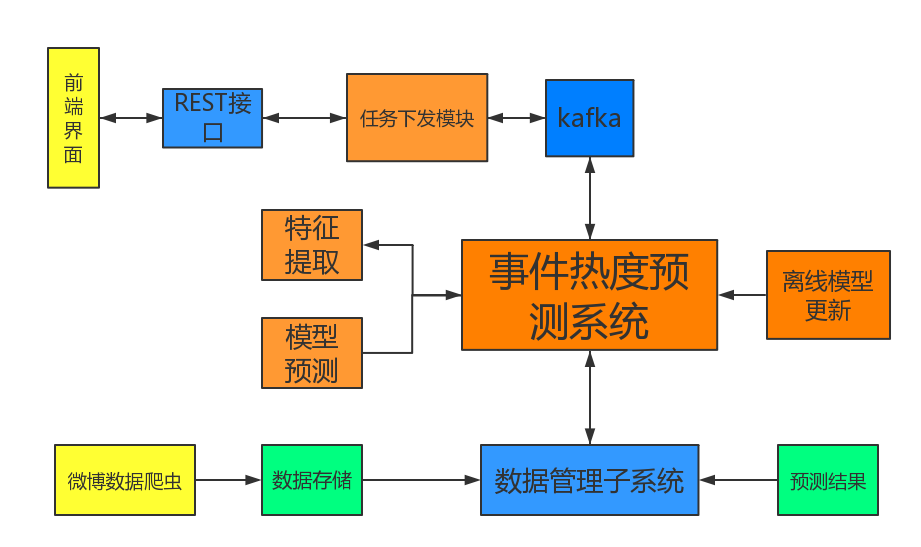
\includegraphics[width=1\textwidth]{5-2}
    \bicaption{系统模块架构图}{System module architecture diagram}
    \label{fig:5_2}
\end{figure}

事件热度预测系统层次架构图\ref{fig:5_3}如图所示,本系统从层次上可以分为四个 层次,从上层到底层可依次分为:展示层、业务层、计算层、存储层。其中展示 层负责数据结果的展示,业务层主要负责完成客户的业务逻辑功能,计算层负责 核心算法的执行,存储层负责业务数据以及结果数据的存储。

\begin{figure}[!htbp]
    \centering
    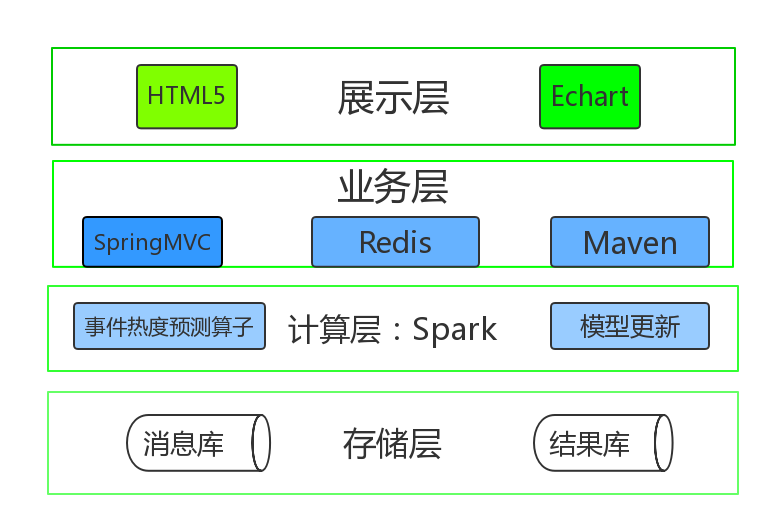
\includegraphics[width=1\textwidth]{5-3}
    \bicaption{系统层次架构图}{System hierarchy diagram}
    \label{fig:5_3}
\end{figure}

\section{微博数据模块}


微博数据模块每天都不断获取新的微博数据,然后进行基本解析,特征提 取,然后入库。微博数据字段如表 \ref{tab:t51} 所示。

\begin{table}[H]
    \centering
    \footnotesize% fontsize
        \bicaption{微博消息表}{Weibo Message Table}
      \label{tab:t51}
    \setlength{\tabcolsep}{30pt}% column separation
    \renewcommand{\arraystretch}{1.2}%row space 
    \begin{tabular}{cccc}
        \hline
         \textbf{序号} & \textbf{属性名称 }& \textbf{属性含义} &\textbf{ 数据类型}   \\
        %\cline{2-9}% partial hline from column i to column j
        \hline
         1 & $wb\_mid$ & 微博消息 ID & $string$ \\
         2 & $cont$ & 微博内容& $string$ \\
         3 & $uid$ & 用户 ID & $string$\\
         4 & $url$ & 微博链接 & $string$ \\
         5 & $nfri$ & 用户朋友数  &$int$ \\
         6 & $nfans$ & 用户粉丝数 & $int$ \\
         7 & $nfwd$ & 转发数量 & $int$ \\
         8 & $nrply$ & 回复数量 & $int$ \\
         9 & $pt$ & 微博发布时间 & $int$ \\
         10 & $loc$ & 微博地域 & $string$ \\
         11 & $message\_type$ & 微博消息类型& $int$ \\
         12 & $wb\_r\_mid$ & 微博根节点 ID & $string$ \\
         13 & $wb\_r\_uid$ & 微博根节点用户 ID & $string$ \\
         14 & $wb\_kw$ & 微博关键词 & $string$ \\
        \hline
    \end{tabular}
 
\end{table}
由于特征较多,一次计算时间过长,本文在获取到微博数据后就进行基本解 析,将其关键词,情感性以及地域信息及时存储,这样需要的时候,可以节约特 征提取的时间开销,当进行事件热度预测的时候就可以及时找到有关数据的特 征,提高系统的性能。



\section{事件预测模块}
本文的事件热度预测模块是根据 Hashtag 的流行度预测模型进行应用的,主 要是将 Hashtag 作为一个事件或者话题进行预测,这样既方便表示具体事件,又 具有一定的用户主观认识。事件预测大致分为三个模块,首先是事件任务下发模 块,这个是根据用户需要,选择相应时间段的微博数据进行分析,根据数据提取 出来的 Hashtag 标签,用户选择相应的感兴趣的事件进行任务下发;其次是事件 预测结果展示模块,根据用户提供的事件以及选择的时间范围,系统自动提取该 时间范围内模型所需的特征,进行事件热度预测,这个过程主要是特征提取的时 间消耗,模型的预测过程是实时响应的,因此后续的优化也主要是集中在特征的 高效提取上;由于微博数据实时更新,对于同一个任务,不同时刻的结果也应该是不同的,因此本文将其进行了自动更新,可以让用户及时查看最新结果。

\subsection{事件任务下发模块}
当用户新建一个任务时,首先需要用户选择观察的时间窗又,因为全量的数 据是庞大的,用户需要选择他感兴趣的时间范围内发生的事件,这样既便于用户 查找结果,也节省了资源的消耗,提高计算速度,新建任务流程如图\ref{fig:5_4}所示。


\begin{figure}[!htbp]
    \centering
    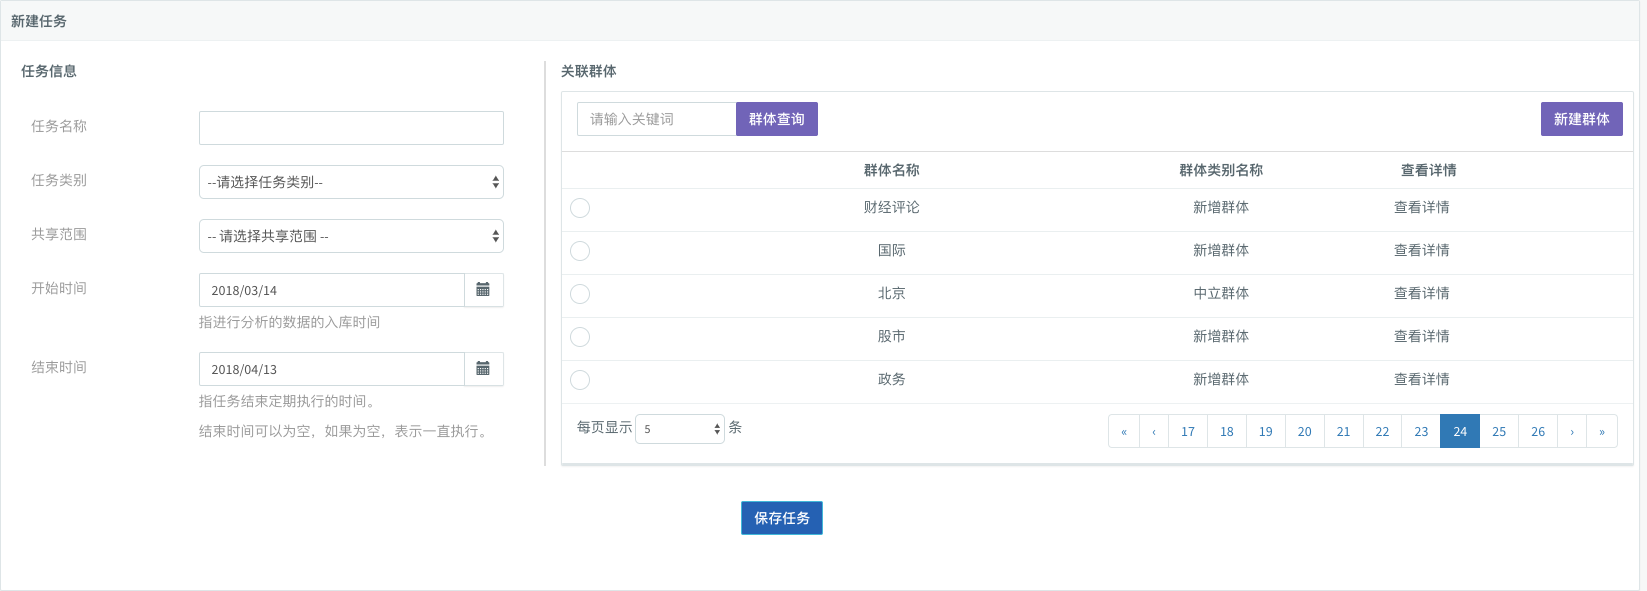
\includegraphics[width=1\textwidth]{hashtag_8}
    \bicaption{ 新建事件热度预测任务}{New Event Heat Prediction Task}
    \label{fig:5_4}
\end{figure}


任务下发以后,后台就根据用户选择的时间范围内的数据进行过滤,筛选, 提取特征,后台利用训练好的模型,对该时间段内的数据特征进行预测,任务等 待结果如图\ref{fig:5_5}所示。

\begin{figure}[!htbp]
    \centering
    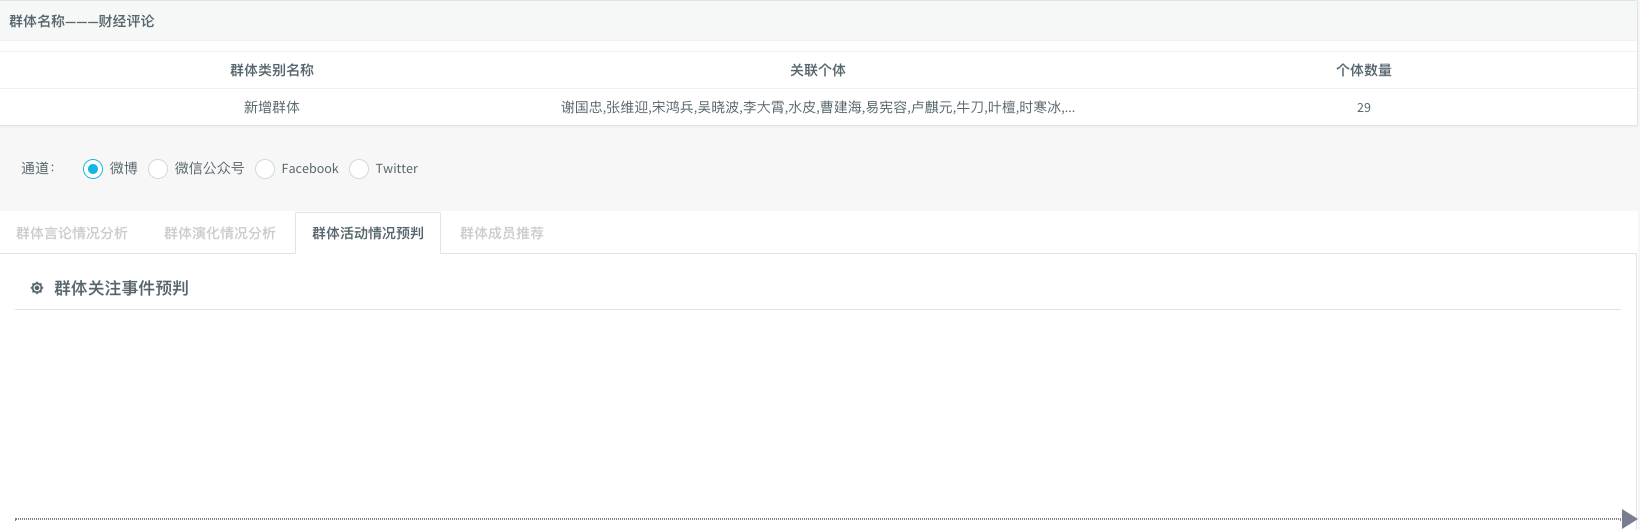
\includegraphics[width=1\textwidth]{hashtag_9}
    \bicaption{事件热度预测任务等待结果}{Event heat forecast task wait result}
    \label{fig:5_5}
\end{figure}

数据库中任务以及结果状态字段如表\ref{tab:t52} 所示,state 字段表示任务执行情况。

\begin{table}[H]
    \centering
    \footnotesize% fontsize
      \bicaption{事件热度预判任务表}{Event Heat Predictive Task Schedule}
      \label{tab:t52}
    \setlength{\tabcolsep}{30pt}% column separation
    \renewcommand{\arraystretch}{1.2}%row space 
    \begin{tabular}{cccc}
        \hline
         \textbf{序号} & \textbf{属性名称} & \textbf{属性含义 }& \textbf{数据类型 }  \\
        %\cline{2-9}% partial hline from column i to column j
        \hline
         1 & $id$ & 任务 ID & $int$ \\
         2 & $name$ &任务 ID& $string$ \\
         3 & $begin\_date$ & 任务开始时间 & $time$\\
         4 & $end\_date$ &任务结束时间 & $time$ \\
        	5 & $state$ & 任务状态& $int$\\
        	\hline
    \end{tabular}

\end{table}


\subsection{事件预测结果展示模块}

系统结果是通过 Kafka 实时反馈的,当系统将模型预测计算完成时,会将状 态位及时写入 Kafka,然后任务的状态位 state 就会显示计算成功, 这样就可以实 时获取计算结果,事件热度预判展示结果如图\ref{fig:5_6}所示。

\begin{figure}[H]
    \centering
    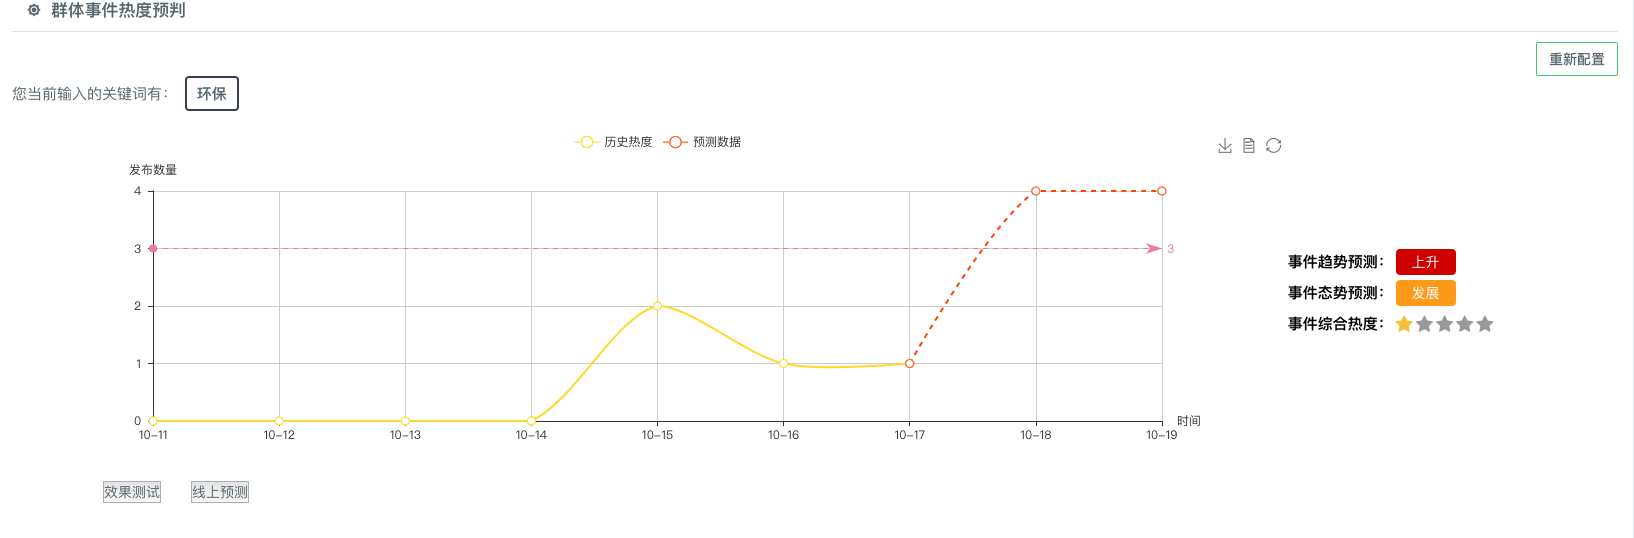
\includegraphics[width=1\textwidth]{hashtag_10}
    \bicaption{事件热度预判结果展示}{Event heat prediction results display}
    \label{fig:5_6}
\end{figure}

在该系统展示效果上,可以查看某一时刻的数据,让用户对该时间发生的事 件有更加清晰的认识,了解该事件的具体内容,数据展示如图\ref{fig:5_7}所示。

\begin{figure}[H]
    \centering
    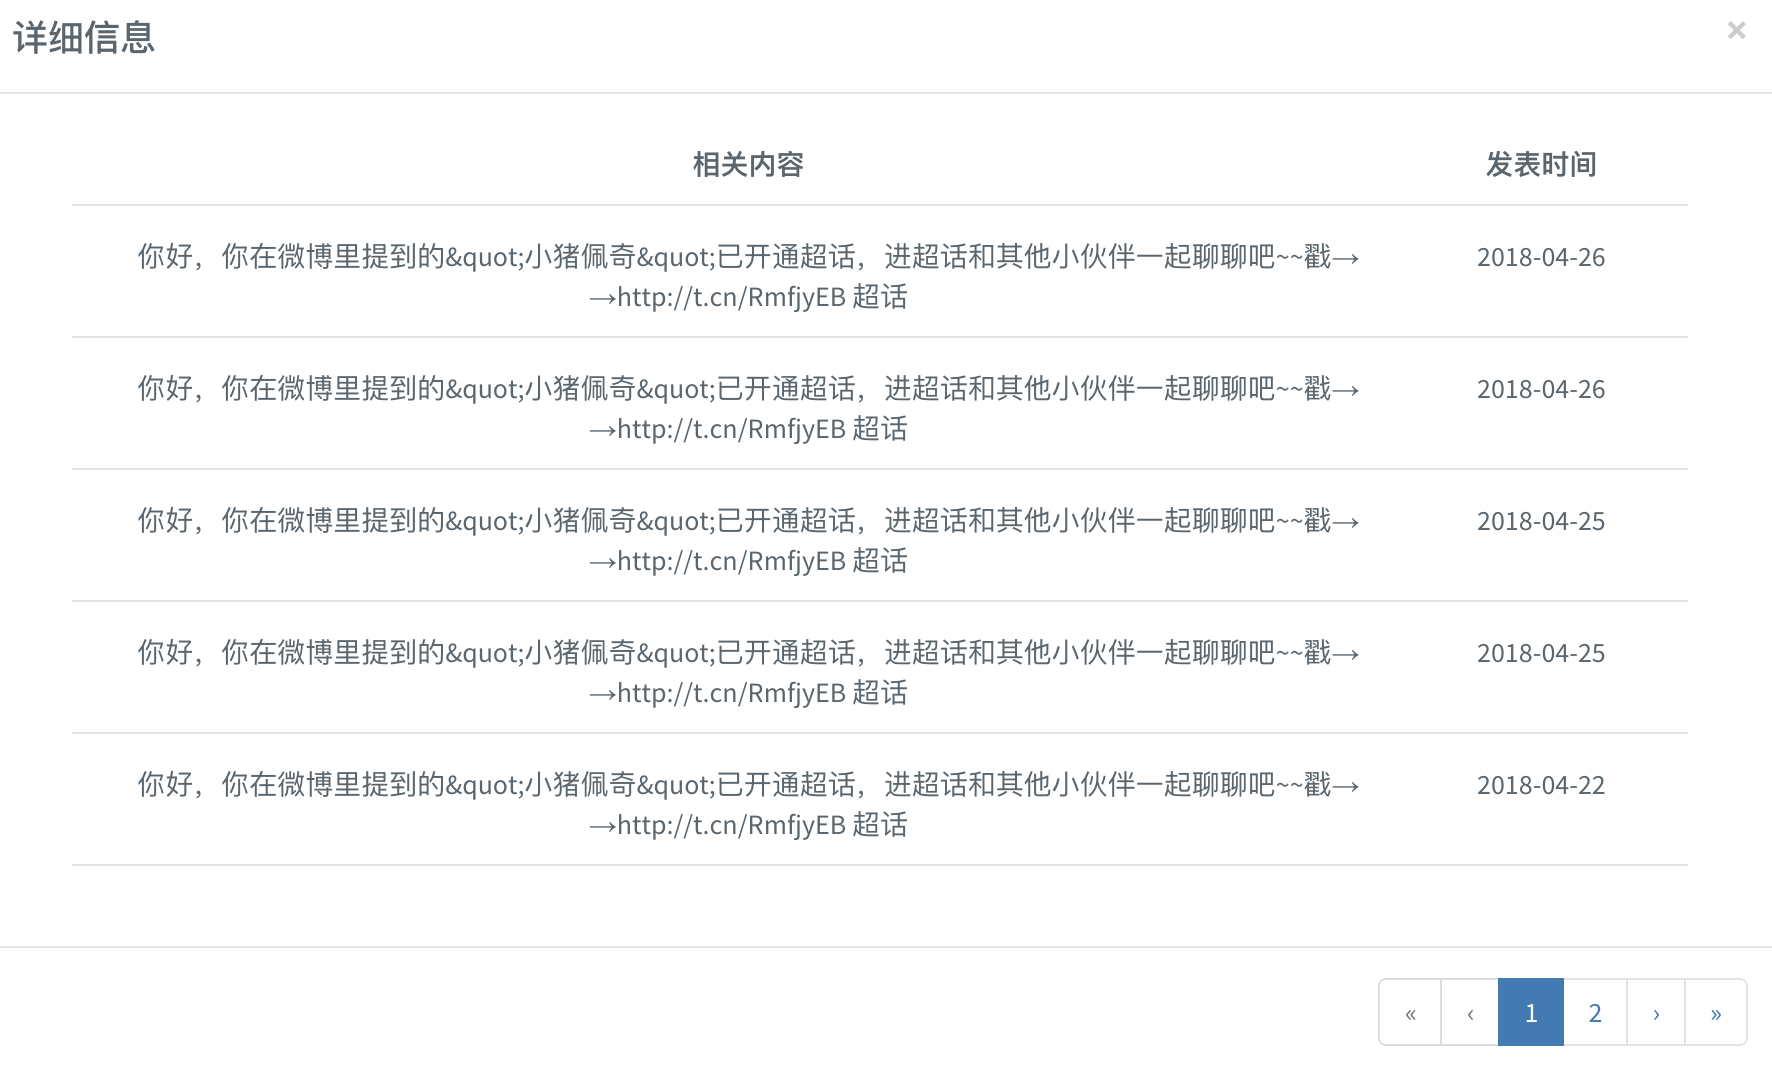
\includegraphics[width=1\textwidth]{hashtag_11}
    \bicaption{事件热度预判下的微博消息展示}{Event heat prediction microblogging message display}
    \label{fig:5_7}
\end{figure}


为了衡量系统的有效性,目前系统设计了线下结果与线上预测的对比,这样 既可以观察系统的有效性又可以给用户对于事件的一个直观长期的认识,效果 如图\ref{fig:5_11}所示,通过线下测试和线上预测的切换,可以查看其历史趋势, 通过之前 的预测结果与目前真实数据之间的对比,可以发现模型的预测结果整体上的趋 势是一致的,数据之间的准确性较高,验证了模型的有效性。


\begin{figure}[H]
    \centering
   
    \begin{subfigure}[b]{0.5\textwidth}
      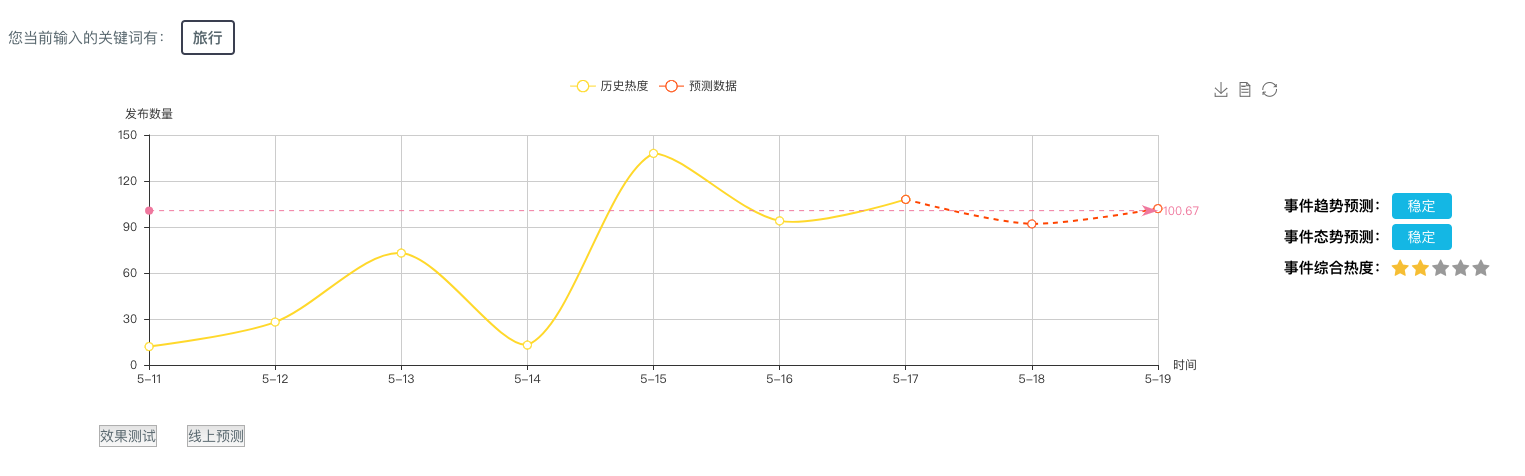
\includegraphics[width=\textwidth]{hashtag_17_new_1}
      \caption{}
      \label{fig:oaspl_a}
    \end{subfigure}%
    ~%add desired spacing
    \begin{subfigure}[b]{0.5\textwidth}
      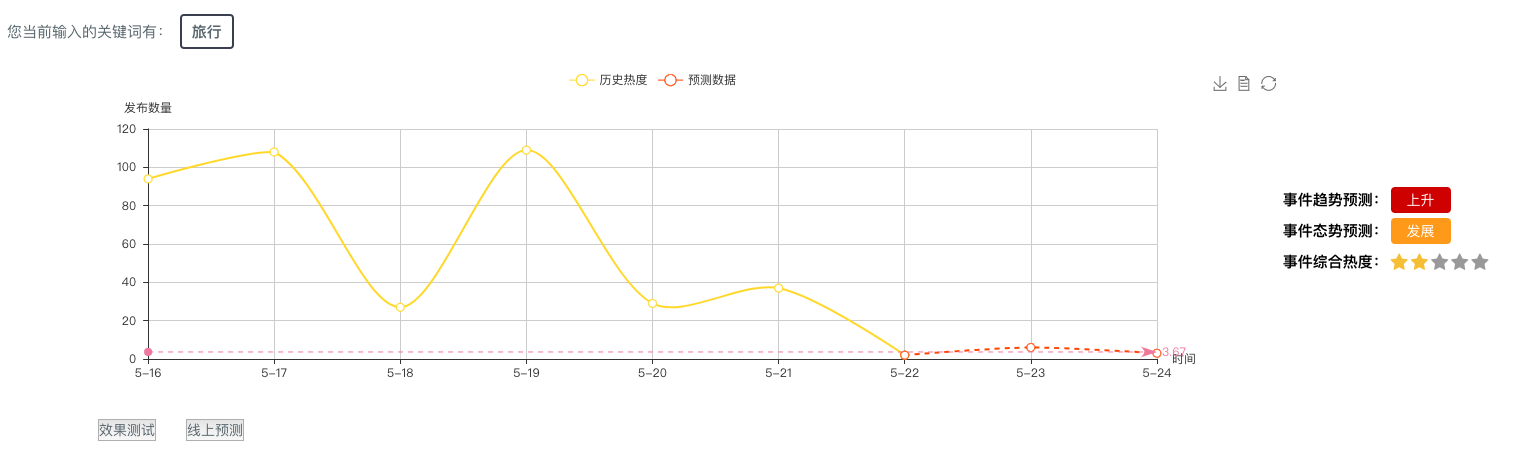
\includegraphics[width=\textwidth]{fig_5_1_2_new}
      \caption{}
      \label{fig:5_1}
    \end{subfigure}
    ~%add desired spacing
     \bicaption{事件预测结果对比。(a)线下预测,(b)线上预测}{Comparison of event prediction results.(a)Offline prediction,(b)Online prediction}
    \label{fig:5_11}
\end{figure}

\subsection{事件自动更新模块}
在本系统中,当用户执行了一个事件热度预测任务以后,由于他可能对此事 件持续关注,希望在长时间内对其了解,便于分析其长期趋势。一般的系统当一 个任务运算完成以后,该任务就处于结束状态,但是在本系统中考虑到数据的实
 时更新,以及用户对于任务的长期关注,本系统设定了任务的自动更新模块,当 用户希望长期关注某一事件以后,可以通过将任务的结束时间设置到未来某一 时刻,这样系统在每天凌晨都会根据结束时间与当前的比对来判断是否更新此 任务,从而实现了该任务的实时更新,确保了用户可以对此事件的长期关注,以 及及时获取最新结果数据。

\section{模型离线训练模块}
由于微博数据的实时性很强,为了能够及时响应最新数据,系统采用线下更
新模型和用户特征数据,这样可以保持一个实时最优模型。

\subsection{微博用户粉丝数据}
系统中包括用户粉丝网络结构的数据,数据结构如表\ref{tab:t53}所示,但是由于用 户关注的群体以及粉丝结构的不断变化,用户粉丝网络结构的向量表示应该实 时更新,但是那样对于系统的资源消耗过大,并且用户的粉丝并不是实时更新 的,短时间内用户粉丝网络结构更新的幅度很小,对于用户向量表示影响很小。 因此系统设计网络结构变化阈值,当用户粉丝结构数量变化达到总体的 10\%,系 统启动用户网络更新模型。

\begin{table}[H]
    \centering
    \footnotesize% fontsize
    \bicaption{微博用户关系表}{Weibo User Relationship Table}
      \label{tab:t53}
    \setlength{\tabcolsep}{30pt}% column separation
    \renewcommand{\arraystretch}{1.2}%row space 
    \begin{tabular}{cccc}
        \hline
         \textbf{序号} & \textbf{属性名称} & \textbf{属性含义} & \textbf{数据类型}   \\
        %\cline{2-9}% partial hline from column i to column j
        \hline
         1 & $fuid$ & 关注用户 ID & $string$ \\
         2 & $luid$ & 粉丝 ID& $string$ \\
         3 & $rlts$ & 用户粉丝之间关系 & $int$\\
         4 & $pt$ &  数据更新时间 & $int$ \\
        \hline
    \end{tabular}
     
\end{table}

\subsection{微博用户向量以及事件预测模型更新}
系统每天会采集大量的微博消息,Hashtag 以及微博消息的特性会随时变化, 它们已有的特征结构可能并不适合未来的事件预测,因此能够及时更新用户特 征,事件特征以及模型,对于预测结果的好坏是十分重要的,因此系统设计每周 末选取一定的数据量,进行用户粉丝网络结构的更新以及 Hashtag 模型的重新训 练,来保证模型的准确性。


\section{系统特色}
本系统具有如下特色:
\begin{enumerate}
\item  \bfseries 实时性 \mdseries 微博数据的采集过程是实时的,并且事件热度预测过程也是实时 更新的,所以整个系统的实时性能够得到保证。
\item  \bfseries 客户端友好 \mdseries 用户在新建任务时候,只需要填写关注时段和关注内容即可, 一键操作,系统可以实现实时更新,便于用户对于任务的查看和管理,并且即使 任务下发以后,用户关注的内容发生变化时,也不需要重新下发任务,只需要更 改关注字段即可,极大的方便用户的使用。
\begin{figure}[H]
    \centering
    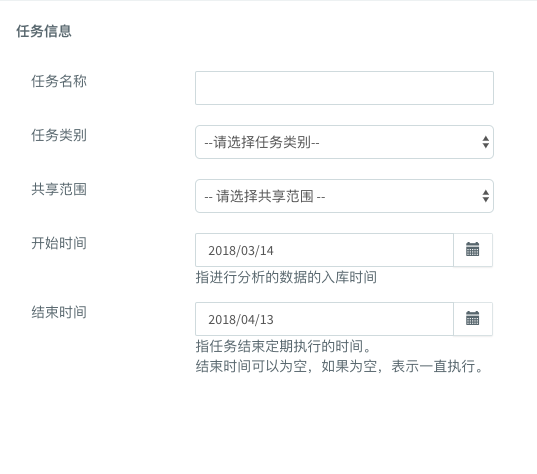
\includegraphics[width=1\textwidth]{hashtag_15}
    \bicaption{微博事件预测任务下发快捷方式}{Weibo event forecast tasks delivered shortcuts}
    \label{fig:5_10}
\end{figure}

\begin{figure}[H]
    \centering
    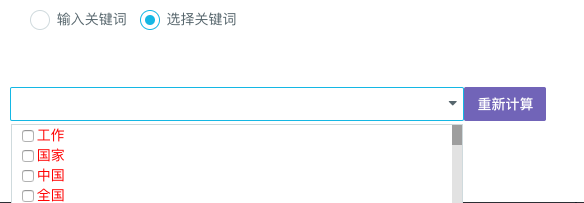
\includegraphics[width=1\textwidth]{hashtag_14}
    \bicaption{微博事件预测更改内容}{Weibo event prediction changes}
    \label{fig:5_9}
\end{figure}

\end{enumerate}

\section{本章总结}

在本文的前两章中,分别介绍了 Hashtag 流行度预测的两种方式,一种基于 特征的宏观预测,一种基于传播过程的多源微观预测。本章在介绍了微博数据采 集的相关情况后,通过将 Hashtag 作为微博的关注事件来进行预测,设计了一个 事件热度预测系统来进行事件热度预测。因为考虑时间效率以及模型的及时更 新,本系统采用基于特征的 Hashtag 流行度预测方式来进行设计,这样便于对结 果的分析。系统能够对采集到的数据以及用户下发的任务进行监控,并且系统可 以及时反馈预测结果,给用户提供了高质量的体验。系统通过对微博事件热度的 预测,能够辅助用户提前得知某一事件的未来趋势,对于评估网民的关注点有一 定的参考,具有较高的应用价值。
\chapter{结论和下一步工作}\label{chap:six}

\section{文章总结}

Hashtag 是微博,Twitter 中一种新的主题标签形式,因为使用简单方便,并 且语意鲜明,可以表达用户主观想法,所以吸引了众多用户参与其中,对其流行 度的预测可以来预测某一事件或者某一话题的热度,因此具有很高的研究价值, 但是目前对于主题标签的研究较少。本文的研究目标是对主题标签流行度进行 预测,贡献如下:
\begin{enumerate}
\item \bfseries 基于用户网络结构特征的主题标签流行度预测\mdseries 

从 Hashtag 自身特性以及用户粉丝的网络结构特性出发,对已有的微博文本 以及时间序列特征进行扩充,提出利用用户粉丝的网络结构向量表示特征,以及 Hashtag 的情感性,地域性,人物性等特征进行模型训练。实验结果表明,新提 出来的特征对于 Hashtag 的流行度预测问题有了一定的效果,也即证明新提出的 特征有效的表达了 Hashtag 的传播特性。

\item \bfseries 基于多源头的主题标签流行度预测 \mdseries 

结合外部知识,利用已有的用户粉丝网络结构作为先验知识,提出多源头的 主题标签流行度预测模型:利用已知的用户粉丝网络结构,学习用户的向量表 达,将其和 Hashtag 的传播路径作为模型的输入进行训练学习,实现用户粉丝网 络结构和多源模型的整合。在大规模微博语料上,对多源模型进行了实验验证。 实验结果表明,模型可以有效地处理多源头的主题标签的流行度预测问题。

\item  \bfseries 建立了一个事件热度预测系统 \mdseries 
事件热度预测的实现与部署,论文考虑到 Hashtag 可以作为微博中的事件或 者话题,采用基于特征的 Hashtag 流行度预测模型,搭建了事件热度预测系统。 事件热度预测系统通过自动分析微博数据,利用本文提出的主题标签流行度预 测算法,进行事件热度预测,通过系统验证了模型的有效性。结果表明,本文提 出的事件热度预测具有较高的应用价值。
\end{enumerate}

\section{下一步工作}

本文的下一步研究内容主要集中在以下几个方面:
\begin{enumerate}
\item  在对主题标签流行度预测中涉及到的特征进行分析后,发现了Hashtag里 面出现的人名以及情感性的重要性,但是在实际的微博消息中,对于更加细致的
 刻画 Hashtag 中的事件性以及不同 Hashtag 之间本质上的区别还是需要更多的研 究工作。
\item 在基于多源头的主题标签流行度预测中,目前考虑了它们最后的融合结 果,但是没有考虑在 Hashtag 传播过程中,多源路径下的用户之间的互相影响, 后续可以试图挖掘不同源头之间的互相影响。
\end{enumerate}
%---------------------------------------------------------------------------%
% main content
%-
%-> Appendix
%-
\cleardoublepage%
\appendix% initialize the environment
%\chapter{中国科学院大学学位论文撰写要求}

学位论文是研究生科研工作成果的集中体现,是评判学位申请者学术水平、授予其学位的主要依据,是科研领域重要的文献资料。根据《科学技术报告、学位论文和学术论文的编写格式》(GB/T 7713-1987)、《学位论文编写规则》(GB/T 7713.1-2006)和《文后参考文献著录规则》(GB7714—87)等国家有关标准,结合中国科学院大学(以下简称“国科大”)的实际情况,特制订本规定。

\section{论文无附录者无需附录部分}

\section{测试公式编号} \label{sec:testmath}

\begin{equation} \label{eq:appedns}
    \begin{cases}
        \frac{\partial \rho}{\partial t} + \nabla\cdot(\rho\Vector{V}) = 0 \ \mathrm{times\ font\ test}\\
        \frac{\partial (\rho\Vector{V})}{\partial t} + \nabla\cdot(\rho\Vector{V}\Vector{V}) = \nabla\cdot\Tensor{\sigma} \ \text{times font test}\\
        \frac{\partial (\rho E)}{\partial t} + \nabla\cdot(\rho E\Vector{V}) = \nabla\cdot(k\nabla T) + \nabla\cdot(\Tensor{\sigma}\cdot\Vector{V})
    \end{cases}
\end{equation}
\begin{equation}
    \frac{\partial }{\partial t}\int\limits_{\Omega} u \, \mathrm{d}\Omega + \int\limits_{S} \unitVector{n}\cdot(u\Vector{V}) \, \mathrm{d}S = \dot{\phi}
\end{equation}

\section{测试生僻字}

霜蟾盥薇曜灵霜颸妙鬘虚霩淩澌菀枯菡萏泬寥窅冥毰毸濩落霅霅便嬛岧峣瀺灂姽婳愔嫕飒纚棽俪緸冤莩甲摛藻卮言倥侗椒觞期颐夜阑彬蔚倥偬澄廓簪缨陟遐迤逦缥缃鹣鲽憯懔闺闼璀错媕婀噌吰澒洞阛闠覼缕玓瓑逡巡諓諓琭琭瀌瀌踽踽叆叇氤氲瓠犀流眄蹀躞赟嬛茕頔璎珞螓首蘅皋惏悷缱绻昶皴皱颟顸愀然菡萏卑陬纯懿犇麤掱暒 墌墍墎墏墐墒墒墓墔墕墖墘墖墚墛坠墝增墠墡墢墣墤墥墦墧墨墩墪樽墬墭堕墯墰墱墲坟墴墵垯墷墸墹墺墙墼墽垦墿壀壁壂壃壄壅壆坛壈壉壊垱壌壍埙壏壐壑壒压壔壕壖壗垒圹垆壛壜壝垄壠壡坜壣壤壥壦壧壨坝塆圭嫶嫷嫸嫹嫺娴嫼嫽嫾婳妫嬁嬂嬃嬄嬅嬆嬇娆嬉嬊娇嬍嬎嬏嬐嬑嬒嬓嬔嬕嬖嬗嬘嫱嬚嬛嬜嬞嬟嬠嫒嬢嬣嬥嬦嬧嬨嬩嫔嬫嬬奶嬬嬮嬯婴嬱嬲嬳嬴嬵嬶嬷婶嬹嬺嬻嬼嬽嬾嬿孀孁孂娘孄孅孆孇孆孈孉孊娈孋孊孍孎孏嫫婿媚嵭嵮嵯嵰嵱嵲嵳嵴嵵嵶嵷嵸嵹嵺嵻嵼嵽嵾嵿嶀嵝嶂嶃崭嶅嶆岖嶈嶉嶊嶋嶌嶍嶎嶏嶐嶑嶒嶓嵚嶕嶖嶘嶙嶚嶛嶜嶝嶞嶟峤嶡峣嶣嶤嶥嶦峄峃嶩嶪嶫嶬嶭崄嶯嶰嶱嶲嶳岙嶵嶶嶷嵘嶹岭嶻屿岳帋巀巁巂巃巄巅巆巇巈巉巊岿巌巍巎巏巐巑峦巓巅巕岩巗巘巙巚帠帡帢帣帤帨帩帪帬帯帰帱帲帴帵帷帹帺帻帼帽帾帿幁幂帏幄幅幆幇幈幉幊幋幌幍幎幏幐幑幒幓幖幙幚幛幜幝幞帜幠幡幢幤幥幦幧幨幩幪幭幮幯幰幱庍庎庑庖庘庛庝庠庡庢庣庤庥庨庩庪庬庮庯庰庱庲庳庴庵庹庺庻庼庽庿廀厕廃厩廅廆廇廋廌廍庼廏廐廑廒廔廕廖廗廘廙廛廜廞庑廤廥廦廧廨廭廮廯廰痈廲廵廸廹廻廼廽廿弁弅弆弇弉弖弙弚弜弝弞弡弢弣弤弨弩弪弫弬弭弮弰弲弪弴弶弸弻弼弽弿彖彗彘彚彛彜彝彞彟彴彵彶彷彸役彺彻彽彾佛徂徃徆徇徉后徍徎徏径徒従徔徕徖徙徚徛徜徝从徟徕御徢徣徤徥徦徧徨复循徫旁徭微徯徰徱徲徳徴徵徶德徸彻徺忁忂惔愔忇忈忉忔忕忖忚忛応忝忞忟忪挣挦挧挨挩挪挫挬挭挮挰掇授掉掊掋掍掎掐掑排掓掔掕挜掚挂掜掝掞掟掠采探掣掤掦措掫掬掭掮掯掰掱掲掳掴掵掶掸掹掺掻掼掽掾掿拣揁揂揃揅揄揆揇揈揉揊揋揌揍揎揑揓揔揕揖揗揘揙揤揥揦揧揨揫捂揰揱揲揳援揵揶揷揸揻揼揾揿搀搁搂搃搄搅搇搈搉搊搋搌搎搏搐搑搒摓摔摕摖摗摙摚摛掼摝摞摠摡斫斩斮斱斲斳斴斵斶斸旪旫旮旯晒晓晔晕晖晗晘晙晛晜晞晟晠晡晰晣晤晥晦晧晪晫晬晭晰晱晲晳晴晵晷晸晹晻晼晽晾晿暀暁暂暃暄暅暆暇晕晖暊暋暌暍暎暏暐暑暒暓暔暕暖暗旸暙暚暛暜暝暞暟暠暡暣暤暥暦暧暨暩暪暬暭暮暯暰昵暲暳暴暵暶暷暸暹暺暻暼暽暾暿曀曁曂曃晔曅曈曊曋曌曍曎曏曐曑曒曓曔曕曗曘曙曚曛曜曝曞曟旷曡曢曣曤曥曦曧昽曩曪曫晒曭曮曯椗椘椙椚椛検椝椞椟椠椡椢椣椤椥椦椧椨椩椪椫椬椭椮椯椰椱椲椳椴椵椶椷椸椹椺椻椼椽椾椿楀楁楂楃楅楆楇楈楉杨楋楌楍榴榵榶榷榸榹榺榻榼榽榾桤槀槁槂盘槄槅槆槇槈槉槊构槌枪槎槏槐槑槒杠槔槕槖槗滙滛滜滝滞滟滠滢滣滦滧滪滫沪滭滮滰滱渗滳滵滶滹滺浐滼滽漀漃漄漅漈漉溇漋漌漍漎漐漑澙熹漗漘漙沤漛漜漝漞漟漡漤漥漦漧漨漪渍漭漮漯漰漱漳漴溆漶漷漹漺漻漼漽漾浆潀颍潂潃潄潅潆潇潈潉潊潋潌潍潎潏潐潒潓洁潕潖潗潘沩潚潜潝潞潟潠潡潢潣润潥潦潧潨潩潪潫潬潭浔溃潱潲潳潴潵潶滗潸潹潺潻潼潽潾涠澁澄澃澅浇涝澈澉澊澋澌澍澎澏湃澐澑澒澓澔澕澖涧澘澙澚澛澜澝澞澟渑澢澣泽浍澯澰淀澲澳澴澵澶澷澸潇潆瀡瀢瀣瀤瀥潴泷濑瀩瀪瀫瀬瀭瀮瀯弥瀱潋瀳瀴瀵瀶瀷瀸瀹瀺瀻瀼瀽澜瀿灀灁瀺灂沣滠灅灆灇灈灉灊灋灌灍灎灏灐洒灒灓漓灖灗滩灙灚灛灜灏灞灟灠灡灢湾滦灥灦灧灨灪燝燞燠燡燢燣燤燥灿燧燨燩燪燫燮燯燰燱燲燳烩燵燵燸燹燺薰燽焘燿爀爁爂爃爄爅爇爈爉爊爋爌烁爎爏爑爒爓爔爕爖爗爘爙爚烂爜爝爞爟爠爡爢爣爤爥爦爧爨爩猽猾獀犸獂獆獇獈獉獊獋獌獍獏獐獑獒獓獔獕獖獗獘獙獚獛獜獝獞獟獠獡獢獣獤獥獦獧獩狯猃獬獭狝獯狞獱獳獴獶獹獽獾獿猡玁玂玃。
% appendix content
%-
%-> Backmatter: bibliography, glossary, index
%-
\backmatter% initialize the environment
\intotoc{\bibname}% add link to contents table and bookmark
\bibliography{Biblio/ref}% bibliography
\chapter[致谢]{致\quad 谢}\chaptermark{致\quad 谢}% syntax: \chapter[目录]{标题}\chaptermark{页眉}
%\thispagestyle{noheaderstyle}% 如果需要移除当前页的页眉
%\pagestyle{noheaderstyle}% 如果需要移除整章的页眉

时光飞逝,转眼间就到了毕业的时间。三年的研究生生活历历在目,忙碌而充实。很高兴也很荣幸能来到计算所,尤其是网络数据重点实验室读研,在此,向所有帮助、关心、支持过我的人表示由衷的感谢。

首先,感谢我的导师廖华明老师。在我的研究生期间,廖老师经常关心我的科研情况,在我研一还在怀柔的时候,在科研内容上,我对自己要做的事情也不是很清晰,这时候廖老师就经常给我发邮件,指导我的学习,提醒我及时复习,学习前沿知识,梳理要做的工作,制定详细的计划,让我可以按部就班的按照计划不断学习与实践,我非常感谢廖老师。在平时的工作中,廖老师以身作则,为人师表,三年来,她兢兢业业和认真负责的工作态度深深影响着我,成为我学习的榜样。

感谢实验室刘悦、伍大勇、俞晓明、周术夏等老师的关心和帮助。实验室的各位老师为我们提供了良好的学习环境,并且时刻关心我们的情况。虽然老师们都很忙,但我们仍然能够有问题就可以去寻找帮助,无论是做人、做事,都受益匪浅。

感谢徐学可老师对我的帮助,进入实验室之初,在徐学可老师的帮助下我对主题模型有了初步的认识,并且他强悍的代码能力让我深深折服,让我对以后的科研有了极大的兴趣。

感谢王永庆师兄,张静师姐带我一起做实际的工程项目,甲方需求变动大,项目联调问题多,很多情况下都是师兄师姐帮我们解决问题,处理不必要的杂事,万分感谢。同时再次感谢王永庆师兄和曹婍同学对我毕设的耐心指导,给了我很多思路和建议,对流行度预测这个方向有了更深的认识。

感谢牛国成、吕福煜、周楠、陈绍毅等舆情组的师兄对我的帮助和支持,和你们一起工作学习受益良多,同时还要感谢同组的岳新玉,赵子承,秦宇君,李飞,王宪发,杨发,张随远同学,从你们身上看到了拼搏,看到了无惧艰险。同时还要感谢我的舍友肖岩,肖岩是一位才华横溢的同学,他自制力强,对未来充满信心,并且十分热爱写代码,对科研也有极大的兴趣,和他做舍友十分荣幸。

感谢研一怀柔同宿舍的马晓龙,宋宇,孔德飞,孙明磊,张远,邓果一,郭邯,肖岩,赵子承这些舍友,在怀柔度过了一年快乐的时光,感谢大家的陪伴和支持,怀念那段青葱岁月。

最后,要特别感谢我的父母,父母给了我学习和生活上巨大的鼓励和支持,给我提供了强大的后盾。特别是感谢父母这么多年的无私奉献和陪伴,在我懵懂无知的时候,与我一起渡过难关。

\chapter{作者简历}


\section*{作者简历}

姓名:王新乐 \qquad 性别:男 \qquad 出生日期:1991.09.10 \qquad 籍贯:河北衡水
\\

2015.9 -- 2018.7\qquad 中国科学院计算技术研究所~\qquad ~硕士 

2011.9 -- 2015.7\qquad 北京科技大学~ \qquad \qquad \qquad \qquad 学士 

\section*{攻读硕士期间参加的研究项目}

\begin{enumerate}[label=\text{[}\arabic*\text{]}]
\item 2016年9月--2017年4月 \qquad 苏州移动主题模型项目
\item 2017年7月--2017年9月 \qquad 社群发现项目
\item 2016年7月--2018年3月 \qquad 舆情监控系统研发
\end{enumerate}

\section*{攻读硕士学位期间的获奖情况}

\begin{enumerate}[label=\text{[}\arabic*\text{]}]
\item 中国科学院大学 \qquad \qquad \qquad ~三好学生
\item 中国科学院大学 \qquad \qquad \qquad ~优秀学生干部
\item 中国科学院计算技术研究所 ~~ ~~优秀志愿者
\end{enumerate}
\cleardoublepage[plain]% 让文档总是结束于偶数页,可根据需要设定页眉页脚样式,如 [noheaderstyle]

% other information
\end{document}
%---------------------------------------------------------------------------%

